\chapter{Euch zum Geleit}

Wir neigen uns dem Ende zu!
Im letzten Teil der Kampagne fehlen uns leider viele Abenteuer.
Das ist natürlich zum einen dem Studium geschuldet, und sicher auch dem Fakt dass niemand mehr großes Interesse daran hatte, nach dem Ende der Kampagne noch weiter zu schreiben.
Die AP hätte man ja gar nicht mehr ausgeben können!

Derrisch ist das hier nun die Darmstädter (und manchmal noch Kelkheimer) Zeit.
In Erinnerung geblieben ist mir natürlich als erstes unser monströser Tisch.
Ich glaube, nicht anderes hat mich in meinem Leben je so sehr den Respekt vor Handwerkern gelehrt wie dieses wackelige Konstrukt.
Über die Jahre hat er Kerzenreste, Pizzaflecken, und viele Erinnerungen aufgenommen, bis ich ihn (glaube ich ?) bei meinem Wegzug aus der Hoffmannstraße entsorgt habe.
Eine besserer Schriftsteller als ich würde hier jetzt noch eine große Lektion oder ein 


\chapter{Auf ein letztes Mal}

Lieber Waldemar,

Dieser letzte Teil der Geschichte wird wohl am kürzesten und fragmentiestark fragmentiert ausfallen. Von den Ereignissen auf der Queste nach den Sieben Kelchen, der Begegnung mit den Trollen, und der grausamen letzten Schlacht sind kaum noch Berichte zu finden.
Dennoch konnte Aria mir zumindest einen extrem detaillierten Bericht über die Schlacht auf den Vallusanischen Weiden zur Verfügung stellen, den Temyr verfasst hatte.
Auch wenn es vielleicht ein Vorurteil ist, aber ich denke, er beweist einmal wieder das Tulamiden unter all den vielen Völkern auf Deren die Wortgewandtesten sind.

Bitte füge die nächsten Zeilen nicht deinen eigenen Berichten zu, sondern verbrenne sie nachdem du diesen Brief erhalten hast. Ich muss dir von einer Geschichte erzählen, die vor einigen Wochen geschehen ist, aber niemand darf von ihr erfahren.

Seit Jahren hatte ich wenig von Temyrs Witwe Aria gehört. Die letzte Information, die ich hatte, war dass sie nach Khunchom gezogen war. Nach der Schlacht hatte sie wohl mehrere Jahre in Drakonia verbracht und bei den Elementarmeistern studiert. Aber nach diesem Exil hat sie eine Stelle an der Akademie in Khunchom angenommen, und ist wohl eine enge Vertraute der Akademieleiterin.

Ich hatte nur wenig Kontakt zu ihr, und sie war immer recht kalt in ihren Briefen. Ich hatte vermutet, dass ihr Schmerz um den Tod ihres Ehemannes einen Kontakt zu mir, oder zu anderen Gefährten aus der Zeit Klammsbrücks zu schmerzhaft für sie machte, und hielt es daher für höflich, nicht aufdringlich zu werden.
Aber mein Projekt, und das der Rhodensteiner, drang immer mehr in jene Zeit vor in der auch sie Teil der Geschichte wurde, und so beschloss ich im Zuge einer Studienreise einen Abstecher nach Khunchom zu machen. Ich wollte die Gelegenheit ergreifen in Temyrs Geburtsort ein paar Nachforschungen anzustellen. Im Zuge dessen erschien es mir angemessen, ihren Wohnort zu erfragen und sie um ein Gespräch zu bitten.

Doch dazu sollte es zuerst nicht kommen! Es war ein heißer Herbstabend, und ich hatte den gesamten Tag in der Akademie über Berichte über den Dämonenkrieg gebrühtet. Mein Tulamyd ist über die Jahre leider sehr rostig geworden, ohne Temyrs blumiges Fluchen in unseren Hallen, und so zog sich meine Arbeit bis zur späten Stunde hin. In der Art alter Menschen vergaß ich, dass es eigentlich zu spät für einen freundlichen Besuch war, und machte mich auf zu Arias Stadthaus.

Als ich auf die Tür zuging, fiel mein Blick durch ein Fenster. Ich weiß, es ist nicht die feine Horasische Art, aber die Neugierde war immer meine größte Sünde. Normalerweise würde ich einer alten Freundin auch nicht nach spionieren, aber was mich erblickte erstaunte mich so, dass ich nicht anders konnte als vorsichtig zu lauschen. Bitte verzeih mir dies!

In Arias Empfangszimmer saßen mehrere in lange, graue Reisemäntel gehüllte Gestalten. Elementarwesen servierten dampfende Getränke, doch das war nicht das auffälligste. Einer von ihnen saß so, dass ich sein Gesicht halb erblicken konnte, und das war es, was mich wie Rondras Donner traf: elfische Züge, die blasse Haut eines Nordmanns, und eine Augenklappe. Es war Firnen! Ich weiß, es ist unmöglich, aber ich schwöre dir, es war Meister Wulfgrimm. Seine Haut war dünn, fast schon Pergamentartig, und seine gesamte Gestalt hatte einen etherischen Character an sich, ich kann es nicht besser beschreiben.

Ich konnte nicht viel vernehmen, aber sie sprachen von Splittern und den Heptarchen! Mir wurde schnell bewusst dass ich nichts davon hören sollte, und ich schlich mich feige davon.

Als ich am nächsten Tag, zu angemessener Stunde, Arias Haus erneut aufsuchte, wurde ich freundlich, aber immer noch etwas kalt empfangen. Aria spielte eine perfekte Gastgeberin, lenkte aber von allen Fragen nach Firnen und Temyr geschickt ab. Ich denke auch um mich ruhig zu stellen gab sie mir den Bericht ihres Ehemannes von den Vallusanischen Weiden und schob mich mit diesem in den Händen fast schon zur Tür hinaus.

Ich werde weitere Nachforschungen antreten und dir als bald von ihnen berichten. Bis dahin überlasse ich dir das Ende meiner Arbeit hier, den finalen Abschnitt über das Wirken der Gezeichneten.

Dein alter Lehrmeister,\\
Iliricon Tannhaus

\chapter{Rohals Versprechen}

\section{Geleitwort}


\begin{flushright}
Claas Völcker, Toronto, den 28.05.2025
\end{flushright}


\section{Die Tagebücher}

\subsection{Der Auftakt des Conventes nach Firnen Wulfgrimm}
\paragraph{01. Ingrimm 1020 Bosparans Fall}
Heute zur Mittagsstunde haben ich und meine Freunde in der Yaquiertaler Hof Unterkunft bezogen. Abgesehen, von einem thorwalsschen Magus, der sich mit einem tulamidischem Magierer über den Preis, eines von dessen Seite aus unverkäuflichem nur wenig magischem Amulett stritt, verlief die Reise problem und ereignislos. Als Begleiter seiner Spektabilität iben Sahid haben wir den überzogensten Luxusflügel bekommen. Wir erwarten noch die Ankunft Torans in den nächsten Stunden, bis spätestens morgen, dann sind wir wieder alle vereint.

Es gild diesen Konvent ausreichend zu nutzen. Meine Verteidigung für die Verhandlung meiner Anklage sollte ich ausreichend untermauert haben bis dahin. Und viele Hypothesen habe ich in den letzten 3 Wochen ausgearbeitet, bezüglich unseres Feindes, und die werde ich nun, in Rücksprache mit den Forschergeistern, die die letzten 6 Jahre sicherlich so manches erdacht haben, zu bestätigen oder Verwerfen suchen.

Viel zu Denken gab mir vor allem das Gespräch mit Talesin von Borbra, den ich jüngst besuchte. Talesin war mit einer Expedition in die Gor aufgebrochen, und war nahe der schwarzen Festung vom untoten Drachen Razzzazor angegriffen worden.
Er meinte al Borbarad seinen Körper in Besitz genommen hatte habe er ein paar Gedanken des Sphärenschänders gesehen. Borbarad suche demnach nach einem irgendwie geartetem Desiderat, eim Schlüssel, der ihm die Sphären öffne. Und wie sich auch jetzt am Drachen zeigt, hat Borbarad trotz seiner Umtriebe im tobrischen immer noch starkes Interesse am alten Zentrum seiner Macht.

Wir unterhielten uns auch über die letzte Schlacht gegen den Bethanier, geführt von Rohal dem Weisen. Wir wälzten ein paar alte Schriften und fanden schließlich eine Abschrift, die den Bannfluch des Los zitierte. Seinerseits gesprochen von Rohal dem Weisen, verschwanden er und der Bethanier darauf hin aus der derischen Sphäre. Rohal riss demnach den Geiste Borbarads mit sich in eine Globule. Zeitlich und räumlich von Dere getrennt sollte niemals ein lebendes Geschöpf, den bösen Geist je wieder beschwören können. Zu blöd das es durch einen Toten geschehen konnte.

Zur borbaradschen Beherrschung bei der Verwendung borbaradianischer Canti ist wohl Cayonon Silberbraue zu befragen. Über die Globulenabschnitte unter Borbra sollte ich mich vielleicht einmal mit Aleya Ambaret unterhalten. Vielleicht schaffe ich es sogar heraus zu finden, wie der Dämon vor Ysilia meinen Schutzzauber umgehen konnte.
Heute Abend ist bereits erstes gemeinsames Bankett in der Akademie. Mal sehen, wen ich dort so antreffe.

Welch ein Disaster. Den Göttern sei Dank dass ich trotzdem jetzt hier sitzen und diese Zeilen schreiben kann.
Meine Reputation ist momentan nicht die Beste vor der weißen Gilde und auch die Graue schaut gespalten auf mich herab. Ich hate gerade erst problemlos alle Sicherheitskontrollen durchlaufen, als ein Rohalswächter auftauchte und behauptete ich sei bereits gekommen. In einm fast einstündigem Verhör unter allerlei magischen Überprüfungen konnt ich schließlich beweisen, das ich der Richtige bin, aber offensichtlich läuft auf dem Konvent ein Doppelgänger umher. Bzw. jetzt da er die Kontrollen passiert hat, ist er in wechselnder oder vielleicht sogar ursprünglicher Gestalt nicht mehr zu finden.

Mit Aleya Ambaret konnte ich bereits srechen und er meinte, dass die derische Sphäre um sich zu schützen. schadhafte Orte einfach abstoße. Als Globule in sich geschlossen liegen sie dort wo sie waren im Limbus verbannt. Wo sich heute das kleine Dorf Borbra befindet, erhob sich in früheren Zeiten, sowohl die Prachtvolle Residenz Assarabads, alsauch die Hallen des Tharsonius von Bethana, der sich Borbarad nennt. Offensichtlich hat Borbarad in früheren Zeiten ebenso an diesem Ort Sphärenrisse entstehen lassen um dämonischen Wessen Einzug zu ermöglichen.

Cayonon Silberbraue war leider nicht Anwesend, aber er hält morgen einen Vortrag, bei dem ich ihn eigendlich erwischen sollte.
Es war ein langer Tag und vor den Anstrengungen von mehreren Tagen Essens, unterbrochen durch mehrstündige Vorträge komplizierter wissenschaftlicher Sprechweise, mindestens in Bosparano gehalten, können wir alle eine gute mütze Schlaf durchaus vertragen.

\subsection{Der erste Vortrag nach Rezzanjin Al'Ahjan}

\paragraph{15.Ingerimm}
Da saßen wir also im großen Puniner Hörsaal als einige von vielen, denn der Hörsaal war bis zum Rand gefüllt und warteten erwartungsfroh auf den ersten Vortrag des Magierkonvents, welches an ebenjenem Tag begonnen hatte.

Doch dieser sollte auf sich warten lassen, da mehrere Weißmagier versuchten den vortragenden, Karjunon Silberbraue, ein anscheinend sehr umstrittener Magier vor allem bei der weißen Gilde, am Betreten des Hörsaals zu hindern. Es ging erst weiter als Firnen Nostrianus Eisenkolber, den Ordensanführer der Pfeile des Lichts mit seiner Anwesenheit ablenkte, sodass dieser seine ganze Wehemenz nicht mehr uneingeschränkt dem Verhindern der Vorlesung schenken konnte. Es ist ganz und gar nicht gut, dass der Kerl, der Firnen offensichtlich nicht leiden kann im Gericht über sein Wohl und Wehe entscheiden wird.

Als der Vortrag dann endlich begann, wurde schnell klar, dass ich unerwünscht bin, da der Vortrag auf Bosparano gehalten wurde. Ich ging also und beschloss den geheimnisvollen Treppenmord mal genauer zu untersuchen. Hierzu musste ich erst einmal herausfinden, ob der ermordete noch im Besitz des Amuletts war, um welches er mit den Thorwaller vor Punin gestritten hatte. Ich fragte also im Borontempel nach dem Verstorbenen Elenviner Magier. Diese hatten die Leiche tatsächlich aufgenommen, die weltlichen Besitztümer jedoch nicht bekommen. Also fragte ich bei Koosmar, dem Organisator des Konvents nach und tatsächlich hatte dieser die Gegenstände aufbewahrt. Da seine Assistentin, mit der ich sprechen konnte, aber nicht herausrücken wollte, ob das Amulett noch in seinem Besitz war, musste ich warten bis sich er selbst der Aufgabe annahm.

Da wir bis zur Mittagsstunden nichts mehr zu tun hatten, beschlossen wir unsere Zeit in der Teestube zu verbringen, wo wir auch Tarlisin von Borbra trafen, welcher gerade einer kleinen Truppe Schaulustiger von seinen Abenteuern berichtete. Anscheinend genervt von diesen übergab er uns die Aufgabe des Erzählers gewandt und machte sich aus dem Staub. Lang und breit erzählte ich daraufhin den versammelten Jungmagiern von den Abenteuern der Gezeichneten. Gegen Mittag wollte ich dann mit den anderen, die beim Vortrag zugehört hatten in der Stadt etwas essen gehen. Doch kaum waren wir auf dem Hof, schon hörten wir einen Schrei aus dem Garten. Schnell eilten wir zum Ort des Geschehens und fanden dort eine panische Elfe, sowie Elcarna von Hohenstein, der über den leblosen Körper eines horasischen Magiers gebeugt war. Neben diesem war ein Weinglas, der Inhalt zum größten Teil auf dem Boden verteilt und der Magier hatte keine sichtbaren Wunden. Man musste also davon ausgehen, dass der Wein vergiftet war. Schon kurze Zeit später kam auch Sirdon Koosmar angerannt und begutachtete den Toten. Ich fragte ihn nach dem Amulett des am Vortag verstorbenen Elenviner Magiers, doch er wusste noch von nichts. Wir überließen den toten Horasier den Magiern zum Untersuchen und gingen essen. Vor der nächsten Vorlesung ging ich nochmal zu Koosmars Assistentin und ließ mir erzählen, dass das Amulett nicht mehr im Besitz des Toten war. Das machte es umso dringlicher den Thorwaller aufzusuchen mit dem er gestritten hatte. Diesen fand ich zugleich in der nächsten Vorlesung und stellte ihn danach zur Rede. Nachdem ich Aleya Ambareth abgewimmelt hatte, der ihn begleitete, stellte ich den Thorwaller zur Rede. Es stellte sich heraus, dass er wohl nichts mit dem Mord zu tun hatte. Darüber hinweg wollte er auch nicht herausrücken, wieso er die Amulette brauchte, da er sie für seine Spektabilität Cellyana von Kunchom sammelte. Darüber hinaus gab er mir zu verstehen, dass diese einen Vortrag über ebenjenes Thema halten würde. Wieder waren wir nicht weiter gekommen. Aber es blieb uns wenig Zeit darüber zu grübeln, da wir uns für den am Abend stattfindenden Ball fertig machen mussten. Er war ein lustiger Abend, wir trafen viele bekannte Leute und feuerten ausgelassen. Doch gegen Mitternacht verschwand Temyr auf einmal und ward bis zum nächsten Morgen nicht mehr gesehen\dots

\subsection{Firnens Urteil nach Irian von Rabenmund}
\paragraph{16. INGERIMM im Jahr 5 nach Borbarads Erscheinen}
An diesem Nachmittag erfolgte die Analyse des Zweiten Zeichens, von der ich nur aus zweiter Hand berichten kann, da ich auf Grund meiner nicht zugehoerig zur magischen Zunft noch den gezeichneten ausgeschlossen war. So wurde anscheinend die Geschichte, wie Toran zu dem Zeichen kam und dessen Faehigkeiten, sowie die passenden Prophezeiungen besprochen.

\paragraph{17. INGERIMM}
Zur Morgenstund hoere ich mir den Vortrag zur Blutigen See an, waehrend die anderen im Vortrag zu den Untersuchungen ueber die Zerstoerung Altaias sitzen.

Am Vormittag finden die Analyse des Dritten Zeichens statt, an der aus oben genannten Gruenden auch nicht teilnehme.

Die wichtigsten Punkte waren, so wurde mir zumindest berichtet, Frage ueber einen Asfaloth-Pakt (Goetter und Daemonen, sind auch nur zwei Seiten derselben Medaille) durch Carolan Schlangenstab, ob es Einblicke in die echsische Kulur gaebe durch den Spinner Muntagonus, sowie Theamtisierung von Rezzanjin's Empathielosigkeit und der Verfolgung der Inkarnations-Theorie.

Gegen Mittag erhalten wir die Einladung zum Zwölfgötterjosten im Rondra in Perricum.

Zum Mittagessen werden wir von Rohezal vom Amboss in einer abgelegen Taverne eingeladen, der Firnen immer wieder besorgten Blicke zu wirft.

Als wir gerade wieder zur Akademie kommen, taucht plötzlich ein Karakilim über Punin auf und laesst den abgeschlagenen mit einer B-Zhayad-Rune gebranntmarkten Kopf von Atavar Friedenslicht fallen, aus dessen toten Mund die bedeutenden Worte kommen:

``Euer Zeitalter ist zu Ende, Kehrt zurueck ins Licht, Fabelwesen!''
Am Abend treffen wir auf Bitten Eternenwachts mit Rumina von Vinsalt und diskutieren mit ihr ueber die Moeglichkeit Borbarad als Sohn Nandus zu verdammen, da diese wehemmt dagegen ist, ein goettliches Wesen seine eigene Goettlichkeit abzuerkennen. Sie leidet gerade als Nandusgeweihte unter den taten den Nandussohns und hat eine Sinneskrise.
Bei unserer Rueckkehr wird Firnen beschuldigt den Magier Veranesco ermordet zu haben.

\paragraph{18. INGERIMM}
Am Morgen des 18. Ingerimms erleben wir, wie der Großmeister der Grauen Staebe, Tarlisin von Borbra, vom Hochmeister der Rohalswaechter Nostrianus Eisenkolber wegen Daemonenbuendelei angeklagt wird. Ein wahrhaft schwarzer Tag für die Einigkeit der Magier!

Wir wohnen Eternenwacht's Vortrag ueber die wachsende Borbarad und Daemonenverehrung in den gefallenen Landen bei, die sorgniserregend beobachtet wird, wozu aber noch keine Problembekaempfung gefunden wurde.
Am Ende des Vortrags erheben die Ucuriaten das Wort und verkuenden für die Welt, dass die Einigkeit der Kirchen für die Kampf wider dem gefallenen Alveraniar oberste Prioritaet hat, so nehmen die Ucuriaten nun Mitglieder aller Kirchen auf und wollen diesen als sacrosankte Botschafter dienen.

Am Nachmittag versammelt sich das Konvent, um über die Zusammensetzung von Rohals's Stein des Weisen zu entscheiden. Zur Dikussion steht, ob man die Onyx-Splitter wieder vereinen soll oder ob man auf Niobara's Warnung hoeren soll. Nach langen Ringen, gerade unter den Anhaengern von Rohals's Lehren, entschließt man sich den Stein des Weisen neu entstehen zu lassen.

Am diesen Abend finden wir uns ein,um dem Urteil ueber die Verfehlungen des Firnen Wulfgrimms zu lauschen.
Das Gericht setzt wie folgt zusammen:

Kläger: Spectabilitus Saldor Foslarin, vertreten durch Hauptfrau Lanzelind Heilenhorst, Pfeile des Lichts

Collegium Iustitium

Hohe Richterin: Spectabilita Racalla von Horsen-Rabemund, Convocata Secunda\\
Erster Gerichtsdiener: Spectabilitus Olorand von Gareth-Rothenfels zu Perricum\\
Zweiter Gerichtsdiener: Archomagus Rohezal vom Amboss\\
Erster Beisitzender: Spectabilitus Nostrianus Eisenkolber, Ordo Defensores Lecturia\\
Zweite Beisitzende: Spectabilita Prishya von Garlischgrötz, Convocata Prima der Grauen\\
Dritter Beisitzender: Archomagus Elcarna Erillion von Hohenstein zu Lowangen\\
Protokollant: Archomagus Carolan Schlangenstab zu Kuslik

Wächter des Argelionsrechts: Inquisitor Parinor von Oppstein\\
Weiser des Argelionsrechts: Magister Erechton, Sacer Ordo Draconis

Die Anklagepunkte lauten:

\begin{enumerate}
\item Besitz und Gebrauch verbotenen Schrifttums nach Codex Band V § 16.1
\item Täuschung der Obrigkeit durch Anwendung der Magie nach Codex Band V § 3.2
\item Kenntnis und Anwendung von untersagten Formeln und Canti nach Codex Band III § 14
\item Falschaussage vor einem Gildentribunal nach Codex Band V § 24.3
\item Flucht vor einem Gildentribunal nach Codex Band VI § 24.2
\item Heimtückischer Mord in zweifacher Ausführung durch Anwendung von Magie nach Codex Band V § 2.1
\item \begin{enumerate}
\item Der Mord an Wachmann Ernst Travian Rondratreu, Stadtwache zu Ysilia
\item Der Mord an Magister Minorum Dexter Hufstädter, Agent der Pfeile des Lichtes
\end{enumerate}
\item Paktierei mit dem Allerunheiligsten Herren der Rache in willentlicher Verleumdung der Zwölfgötter und aus niedersten Beweggründen Codex Band I § 14.1
\item Entzug als angeklagter Seelenpaktierer aus der Gerichtsbarkeit der Gilden durch den unter 6.1 genannten Mord nach Codex Band V § 2.3
\end{enumerate}


Im ersten Punkt kommt es zu einem Freispruch aufgrund eines Formfehlers der Anklage, er muss aber ein Bußgeld von 10 Dukaten bezahlen.

Unter Punkt 2 wird Firnen im Punkto: Anmaßung eines anderes Standes, als nicht schuldig angesehen, aber schuldig gesprochen für die Aneignung von mittelreichischem Staatseigentum, was an ein weltliches Gericht verwiesen wird.

Firnen gibt die Kenntnis von Tempus Stasis und Verbotenen Pforten zu und muss deshalb 10 Dukaten Bußgeld zahlen. Die Anklage zur Beherrschung der Blutmagie und der heptasphaerischen Invocation wird allerdings zurück gezogen.

Punkt 4 wird von der Anklage zurückgezogen.

Bei Punkt 5 müssen die besondern Umstaende beachtet werden unter denen sich Firnen für schuldig erklaert.

Bei beiden Morden wird Firnen wegen Mangel an Beweisen fuer unschuldig gehalten. Ihm wird aber vertretbarer Totschlag vorgehalten und er hat schon wieder ein Bußgeld von 10 Dukaten zu zahlen.

Firnen leugnet den Daemonenpakt nicht, haelt aber seinen Kampf gegen Borbarad und Seine Schergen dagegen.

Schlußendlich wird der Magier Firnen Wulfgrimm als schuldig in den Hauptanklagepunkt gesehen. Er wird aber aufgrund seiner Verdienste wider dem Nanduszwilling nicht der Purgation unterzogen, sonder aus der Großen Grauen Gilde des Geistes verbannt.

\subsection{Das Auffinden des Mörders nach Temyr ibn Sahid}

\paragraph{19. Ingerimm im Jahre 1020 nach dem Falle Bosparans}
Am nächsten Morgen begaben wir uns direkt nach dem Frühstück in die Hallen der Akademie zurück, um dem traditionellen Götterdienst oder der Konkurrenzveranstaltung des Tomeg Aterion -- ``Warum wir nicht im Götterdienst sind'' -- beizuwohnen. Die Inhalte der letzteren lassen sich freilich in einem äußerst populären tulamidischen Sprichwort zusammenfassen, dessen Erklärung hier aber zu weit gehen und die leutseligen Gemüter meiner Gefährten unnötig belasten würde\dots Kaum hatten wir uns jedoch hernach wieder zusammengefunden, als Sidor Kosmaar mit ahnungsvollen Schritten herangeeilt kam und unsere Sorgenliste um einen weiteren Punkt ergänzte. Der Mörder, dessen verachtenswertes Geschick schon die letzten Tage den Konvent in Atem gehalten, hatte ein weiteres Opfer gefordert: eine junge Magistra namens Yaneska Yanolof, die auf dem Weg zu ihrer Herberge erdrosselt aufgefunden worden war.

Was war das Ziel des Attentäters? Wie stand er in Verbindung mit den Plänen des Thorwaler Magus und seiner Vorgesetzten, Seliana von Khunchom, in welche Rezzanjin Einblick zu gewinnen versucht hatte? Und war es eben dieser, der bereits am ersten Tage in Gestalt Firnens den Konvent aufgesucht hatte? Über all diese Fragen diskutierten wir reiflich und hitzig, und griffen dabei einen Gedanken auf, den Firnen als erster gefasst hatte, nämlich die Identität des Assassinen betreffend. Handelte es sich bei dem Schurken, der ja in der Kunst der Magie durchaus bewandert schien, um einen der abtrünnigen Tuzaker Magier, die so früh schon unsere Pläne gestört hatten? Wenn ja, so würde er mit Sicherheit auch hinter uns selbst her sein, und seiner Chance unter allen Umständen harren. Die Überlegung schien naheliegend, und so fassten wir den Plan, dem Täter eine falsche Fährte auszulegen und seiner in persona habhaft zu werden. Als Ausleger der Falle wählten wir meine feierliche Ernennung zum Erzmagus, der sich nach guter tulamidischer Tradition eine weniger offizielle, aber dafür weitaus ausschweifendere Festivität anschließen musste. Mit meinem Kopf in Reichweite, so folgerten wir, würde es dem Mörder eine unwiderstehliche Verlockung präsentieren, erneut zuzuschlagen. Nur dass in diesem Augenblick, selbstverständlich, wir selbst zuschlagen würden\dots

Wir besprachen den Plan in aller Eile, aber gebotener Vorsicht mit der Magistra Prima von Garlischgrötz, die unserem Vorhaben zustimmte und erste Vorbereitungen in die Wege leitete. Als wir uns zurück in das Gedränge des Konvents begaben erreichte uns eine Depesche des Hesindetempels, welche zur Audienz bei der ehrenwerten Haldana von Ilmenstein lud. Nach dem letzten Vortrag des Tages, in welchem Dscheleff in einer flammenden Rede den Zusammenhalt der Magierschaft beschwor und zur Unterstützung der Gezeichneten aufrief, verließen wir die Hallen der Akademie am Nachmittag und wandten unsere Schritte zum Haus der weisen Göttin. Die Magistra der Magister empfing uns freundlich und dankte für unsere Bemühungen im Kampf gegen Borbarad. Ebenso lag es ihr jedoch daran, Erkundigungen einzuziehen, worin wir ihr mittels eines ausführlichen Berichts aushelfen konnten. Über unser Auskünfte war es schon Abend geworden, und die Geweihte hieß uns zu bleiben für ein Treffen von Hesinde- und Magiergeweihten. Uns so trafen dann im Herzen der Nacht, zur Hesindestund, die Geweihten der Göttin ein, um die allgemeine Verdammung des Borbarad vor den Augen von Göttern und Menschen zu beschließen. Die höchsten Geweihten des Phex, des Nandus' und der Hesinde traten um den Altar, und mit donnernden Stimmen, die nicht Menschen, sondern Göttern gehörig waren, verkündeten sie das Wort vom einigen Ratschluss. Ein würdiges und gerechtes Zeichen im Angesicht eines Götter und Menschen verachtenden Gegners!

\paragraph{20. Ingerimm}
Der folgende Tag begann mit einer gewaltigen Überraschung, der sich noch weitere anschließen sollten -- gute wie schlechte. Als wir nämlich wie üblich unsere Schritte zum Pentagrammaton lenkten, versperrten uns dort die Rohalswächter unter Nostriamus Eisenkolber den Weg. Selbiger trat mit gequälter Miene vor und übergab Toran mit zitternden Händen seinen Onyxstab, den er zuvor unter keinen Umständen herzugeben bereit war. So erstaunt waren wir über dieses kleine Wunder, dass wir kein Wort hervor brachten -- im Gegensatz zu Eisenkolber, der uns mürrisch beschimpfte und auch sonst wieder ganz der Alte zu sein schien. Mit diesem Schatz in den Händen begaben wir uns ohne Umschweife zu Seliana von Khunchom, die über alle Maße erfreut über einen Stein dieser Größe war. Danach widmeten wir uns weiterhin der Vorbereitung unserer Falle, bis die ersten Vorträge des Abends unsere Aufmerksamkeit verlangten. Abermals teilten wir uns unserer Interessen gemäß auf und besetzten verschiedene Hörsäle, um das Angebot des Konventsplans auszuschöpfen. Der Vortrag des Khadil Okharim beleuchtete die Fortschritte bei der Erstellung des bastrabunschen Bannschildes, an welchem wir selbst tatkräftig mitgewirkt hatten. Die Rekonstruktion der Bannformeln schien gut voranzugehen, doch hatten sich tiefere Probleme bei der Entschlüsselung der materiellen Komponenten der Spruchform aufgetan. Magister Okharim war gerade dabei, die feineren Züge seiner Analysen zu erläutern, als auf dem Flure ein unglaublicher Tumult ausbrach und die versammelte Magierschaft in heilloses Durcheinander stürzte: Während des parallelen Vortrages der Magistra von Garlischgrötz hatte sich, wie Firnen später atemlos berichtete, ein Riss im Sphärengefüge aufgetan, aus welchem sich unaufhörlich Zantim ergossen und die Zuhörer angegriffen hätten. Irgendwie gelang es zwar, den Dämonen Herr zu werden, aber unter welchen Verlusten! Viele hatte die Dämonenbrut hingemetztelt oder schwer verletzt; das eigentliche Unglück wurde aber erst später offenbar. Im Schutze der Verwirrung und Panik waren nämlich die gesammelten Onyxsplitter aus den Räumen der Seliana von Khunchom entwendet worden, nicht ohne ihrem treuen Untergebenen Ilachim die Kehle durchzuschneiden.

Nun hieß es, auf das Gelingen unserer Falle zu bauen und den Mörder, wenigstens jedoch die Steine, zurückzubringen. Nachdem der feucht-fröhliche Abend im besten Gasthaus Punins ausgeklungen war, begab ich mich allein durch die nächtliche Gassen der Stadt zurück zu unserer Unterkunft -- stets gedeckt von den unsichtbaren Schatten meiner Freunde, die mir unauffällig folgten. Und tatsächlich dauerte es gar nicht lange, bis sich der Unhold aus seinem Versteck begab. ``Paralysis!'' hörte ich hinter mir eine Stimme schreien und eine Welle magischer Energie brandete über mich hinweg. Da ich aber mit einem solchen Zug gerechnet hatte, gelang es mir den Zauber abzuschütteln und dem Magus -- es handelte sich tatsächlich um einen Maraskaner -- einen saftigen Ignifaxius entgegen zu schleudern. Sogleich sprangen meine Gefährten hervor und warfen sich in das Kampfgetümmel. Der Magier hatte mit so viel Gegenwehr freilich nicht gerechnet und versuchte sofort, dem Kampf zu entgehen: Sein ganzer Körper schien in sich zusammenzufallen, zu schrumpfen, da wuchsen schwarz-ledrige Schwingen daraus und mit raschem Flügelschlag verschwand der Blutsauger in der Nacht. Rezzanjin jedoch rannte, von der Kraft eines Zaubers erfüllt, hintendrein, und konnte den Maraskaner bis zu einem verfallenen Turm verfolgen, in dessen labyrinthischen Eingeweiden er den Kerl aber verlor. Als der Rest von uns endlich mit menschlicher Geschwindigkeit dort eintraf, hatte Rezzanjin bereits das ganze Versteck auf den Kopf gestellt und neben den Steinen auch einen Brief entdeckt, der an einen gewissen Torben Dergeler adressiert und von unserer alten ``Freundin'' Azariel Scharlachkraut unterschrieben war. Offfenbar hatte sich die Hexe noch bis gestern selbst in Punin aufgehalten und hatte das Wirken des Tuzakers überwacht. Weiterhin enthielt das Schreiben Anweisung, eine gewisse Hexe aus Maraskan namens Lavinia aufzusuchen, sobald der Auftrag erledigt wäre. Wenigstens dem hatten wir einen Stich versetzen können. Mit den Steinen im Gepäck begaben wir uns zur Akademie.

\paragraph{21. Ingerimm}
Das Arbeitskabinett der Convocata Prima war schon bis auf den letzten Platz ausgefüllt, als wir tags darauf auf dem Konvent eintrafen. Seliana von Khunchom hatte bereits die Fakten rund um die Onyxsteine und ihre Arbeit resümiert, und erging sich dann in weiteren Ausführungen über die nun zu beschließende Vorgehensweise. Zunächst einmal galt es, für den Stein der Weisen die fähigsten Artefaktmagier, Analysten und Handwerker auszuwählen, die diesem delikaten Gegenstand Form verleihen sollten. Die anwesenden Magier diskutierten wohl manche lange Stunde, bis endlich die fünf Betreffenden zusammengestellt waren. Der Ratschluss lautete auf: Salpicon Savertin, Firnen Wulffgrimm, Salandrion Farnion Finkenfarn, Ragnos vom Svelltal und mich, Temyr ibn Sahid. Das Wunder konnte vollzogen werden.

\subsection{Der Stein der Weisen nach Firnen Wulfgrimm}

\paragraph{21 Ingrimm 1020 Bosparans Fall}
Der Stein des Weisen soll nun beschlossener Maßen wieder zusammen gesetzt werden. Sowohl Temyr als fähiger Artefaktmagierer, als auch ich, mit meinen überdurchschnittlichen Analysefähigkeiten, werden dabei mithelfen dürfen. Da Temyr sich bereits ein paar Gedanken machen wollte, über eine mögliche Artefakt Thesis, zur Reaktivierung der vorhandenen Strukturen, analysierten wir noch einmal einen Großteil, der Splitter. Dabei erregte Zulhamid in mir einen schrecklichen Verdacht. Ich wollte soeben einen Analys zaubern, da offenbarte mir der Magiermogul bereits den gewünschten Anblick. Er war völlig aus dem Häuschen und wollte keine Sekunde länger mit dem Zusammensetzen warten. Die magischen Strukturen trügen SEINE Signatur, die Art und Weise, des Assarabat, beziehungsweise des Bethaniers, und das Artefakt brächte uns einen Weg IHN zu finden. Was ist nun, wenn wir weder Kontakt zu Rohal erreichen, noch ihn beschwören können, sondern den Bethanier rufen? Ich vermag mir dieses Schreckensszenario kaum auszumalen. Das Artefakt ist unsere einzige Handlungsmöglichkeit und ich bete zu den Göttern, dass sie uns etwas Gutes bringt.

Toran kam kaum später herein. Er hatte im Tempel meditiert und eine beunruhigende Ahnung hatte ihn erreicht. In Gedanken an die Göttin, sah er einen Turm wie aus Glas und goldene Schuppen, und ein ungutes Gefühl beschlich ihn, dass ihn jetzt noch frösteln lässt, wenn er daran zurückdenkt. Der einzige unsichtbare Turm, er wird eigentlich nur durchscheinend, den ich kenne, ist der Hofmagierturm im Ambossgebirge. Derzeitig verwahrt und bewohnt von Rohezaal vom Amboss.

Wir wollten Rohezaal von unseren Theorien und Befürchtungen in Kenntnis setzen, doch er bat uns ihn erst am frühen Abend in der kleinen Bibliothek zu treffen. Torans Vision könnte eine seiner Theorien bestätigen.

Rezzanjinn beschloss uns zur Unterredung zu begleiten, Irian hatte schon am Mittag die Stadt verlassen, warum wusste keiner. Tatsächlich erwartete uns Rohezaal bereits in der kleine Bibliothek. Er hob gerade zu sprechen an, uns eine Mitteilung immenser Bedeutung machen zu müssen, als er nach vorne sackte. Ein kleiner Borndorn ragte aus seinem Nacken. Während Toran, Temyr und ich uns erfolgreich bemühten den Erzmagier im Leben zu halten, bemühte sich Rezzanjinn den bereits bekannten Maraskaner, der hinter einem Vorhang verborgen gestanden hatte, dingfest zu machen. Trotz eines abgeschlagenen Armes, entkam der Asfalothpaktierer als Vogel durch das Fenster. der Arm wuchs nach. Rohezaal erklärte uns von einem Hexagramm aus Orten, die mit Rohals Wirken zu tun gehabt haben. In der Mitte des Hexagramms der Ort Wagenhalt, in dem Rohezaal der Legende nach erschien. Rohezaal glaubte, das der weise Magier im Falle einer Beschwörung, über diese Orte seinen Weg gehen würde von einer geistigen Gegenwart, bis zur Verkörperung. Sobald sich die Theorie bestätigen würde, wolle er in den Amboss reisen, und versuchen, eine Verkörperung zu verhindern, den usn allen klingt noch immer die Warnung Nihobaras von Anchopal in den Ohren: "Niemals vollendet sei der Ruf nach den Beiden, um göttliche Allmacht auf Deren zu meiden." Der Plan Rohezaals klingt verrückt, aber er könnte klappen.

Eine geraume Zeit schon von unseren Stäben, durch ihre Zerstörung entbunden, beschlossen Temyr und ich ihre Spektabilität zu Punin zu bitten, uns Material aus den Akademiegewölben nehmen zu dürfen, um uns neue Stäbe zu erschaffen. Die Bitte schlug sie uns nicht ab, und nun wird sich zeigen, ob wir in einer Nacht zu vollbringen vermögen, zu dem der Eleve knapp eine Woche benötigt.

Ich fand einen knorrigen Stab von etwa eineinhalb Schritt Länge, aus dem Holz der Steineiche, das ich nicht im Besitz einer Punier Akademie vermutet hätte. Vielleicht war es ein Experiment gewesen, das die Akademie einst beschlagnahmt hatte, denn es befand sich in die Verästelung am oberen Ende des Stabes geschnitzt, eine ebenso ungewöhnliche Walrune, wie bei den Thorwalern üblich. Die Verästelung beinhaltete bereits eine Fassung, nur der Stein schien abhanden gekommen zu sein. Ich fand passend einen bordeaux farbenen grobbehauenen Topas, den eine Silberne Mondsichel zierte.

Das Holz scheint eine ungewöhnlich große Affinität zu Blitzen und Feuer zu haben. Der Stein hat eine eigene antimagische Kraft. Die Walrune hat sich magisch mit der silbernen Mondsichel verbunden. Es muss eine Art thorwalsches Zauberzeichen sein, es wirkt der Verständigung zugehörig. Kaum hatte ich den Stein in den Stab eingesetzt, erschienen magische Zeichen, des Feuers und der Antimagie in silbrigem Arkanum, und ebenso Flammen die, sich um den Stab rankend, diesen schmücken in unvergleichlicher Weise. Ich denke der Stab ist passend wie kein zweiter. Und ich danke den Götter für die merkwürdige Vielfalt der Sammlung einer so alten Akademie wie der in Punin.

Etwa zwei Stunden vorm Weckruf der Kirchenglocken traf ich Temyr in der großen Halle der Akademie. Er war ebenso fertig geworden. Es war ihm gelungen einen etwa zwei Schritt langen Stab aus Rashtulszeder zu bergen. Nun schmückte ihn zu dem ein Amethyst in Form einer stilisierten Rose.

Müde und zufrieden kehrten wir in unser Gasthaus zurück. Wenigstens die letzte Stunde werde ich noch zu schlafen versuchen, bevor vielleicht der Größte Tag seit langer Zeit anbricht.

\paragraph{22. Ingrimm 1020 Bosparans Fall}
Es bereits Abend ich bin gleichermaßen erschöpft und verstört. Die Ereignisse des Tages übertreffen fast alles bisher erlebt an Unvorstellbarkeit. Doch bei allem Schrecken bleibt ein Schimmer der Hoffnung.

Also von Vorn: Wir begannen bereits zu früher Stunde mit der Rekonstruktion des Steins des Weisen. Die bereits angefertigten detaillierten Analysen erleichterten das Vorankommen erheblich. Stück für Stück setzte sich das Artefakt zusammen, und obgleich es ungemein Kräfte zehrend war, dauerte es nur wenig Stunden. Das ungeheuerlichste Artefakt, das ich je gesehen hatte war zusammen gesetzt worden. Ein Schwarzes Auge, in Form einer etwa Kopfgroßen Kugel, das nicht die Zeit, sondern die Spähren zu durchblicken scheint, und eine Invokation herbeiführen konnte die nicht der siebten Sphäre zugeordnet werden kann.

Die drei Konvokati Primae der Gilden legten ihre Hände an das Artefakt und schienen in Trance zu versinken. Bilder zogen durch den Raum, Bilder jener Orte, die Rohezaal dem Hexagramm zugeordnet hatte. Er schien also in seinen ersten Punkten Recht zu behalten. Er bat uns ihn zu seinem Turm zu begleiten, und mit ihm flogen wir auf seinem Freund, Faldegorn, einem Kaiserdrachen, ins Ambossgebirge.

Tatsächlich offenbarte sich uns dort das gelegentliche aber seltene Spektakel, den unsichtbaren Turm zu sehen, in der durchscheinenden spiegelnden Art, die ihm im Volksmund diesen Namen einbrachte. Rohezaals Tochter eilte uns entgegen. Sie sagte alle Tiere habe die Gegend verlassen, beziehungsweise, haben sich auf einer Bergwiese, ein Stück unterhalb des Turmes gelegen, versammelt. Auch wir eilten schnellen Schrittes zu dieser Wiese und tatsächlich: Als wir dort ankamen bot sich uns ein Anblick, den ich auf immer in meinem Herzen tragen werde. Aus den leichten Schwaden eines Bergnebelfeldes heraus kam ein Mann geschritten. Seine Haltung edel, sein Gang bewusst und rechtschaffend, sein Blick voller Güte und seine Worte voll Weisheit. Sein Wesen voller Freundlichkeit. Rohal war zurückgekehrt. Als wir mit seiner Hilfe unsere Sprache wieder fanden, bedrängten wir ihn schließlich doch mit den dringlichsten Fragen, die uns seit geraumer Zeit nun schon, so arg beschäftigten. Was sollten wir unternehmen um Borbarad aufzuhalten? Rohal sah uns unsere Zielstrebigkeit nach, auch wenn er uns ermahnte stets auch die Welt im Auge zu behalten, wenn wir unseren Weg zu sehen versuchen. Er verriet uns die Schwachstelle Borbarads: Der Bethanier hat Satinav um seine Zeit gebracht, als er sich zurück holen ließ, und mehr denn je hat er seine Zeit verkauft. Wenn wir den Bethanier nun zu hindern gedächten, so sollten wir seine Zeit finden und hüten. Diese Aufgabe übertrug er uns und im besonderen Temyr, dem er zum Zeichen seines Auftrages, die Kappe des Weisen auf sein Haupt setzte. Der fünfte Gezeichnete ist erschienen. Er trägt das Zeichen der stählernen Stirn und das Wissen um seinen Frevel.

So erleichtert über die Einsicht in die Tiefen der Welt und die begründete Hoffnung auf ein Morgen, standen wir ahnungslos auf der Bergwiese und redeten noch von Angesicht zu Angesicht mit dem Weisen persönlich, als das Unheil heraufzog. Der Himmel verfinstert sich und die Vögel hatten längst das Weite gesucht, als sich die Sphären öffneten und Borbarad hervor trat. Auf seinem Haupt trug er, und noch jetzt schaudert mich die bloße Erinnerung dieses Anblicks, die siebenstrahlige Dämonenkrone. Sieben Erzdämonen hatte er seine Seele versprochen in der Gewissheit, dass sie sie nie würden fordern können. Sie sollten sich selber gegenseitig zerfleischen, um den größten Schatz der Niederhöllen, seit der Versuchung des Namenlosen, die Seele des Alveraniers des verbotenen Wissens.

Borbarad lachte Rohal aus, ob der Schwäche ihn nicht vernichtet zu haben, er beschämte die Liebe die ihm der weise Zwillingsbruder entgegenbrachte, überhörte die Warnungen und den Rat. Er lästerte seines Unvermögens auf die Hilfe des Los angewiesen zu sein, und sprach den ebenso schrecklichen wie verächtlich kurzen "Bannspruch des Borbarad": "Rohal sei nicht mehr!" wir wollten fliehen, wie Rohal uns als letzte Worte riet, doch der Bethanier hielt die Zeit, und ließ sie nach seinem Willen fließen. Wir mussten mit ansehen, wie Rohal langsam verblasste, bis er schließlich verschwand. Unsere Freiheit erlangten wir erst wieder, als Borbarad sich abwendete. "Zerreißt sie!", sprach er und überließ einem Dutzend Zants das Feld. Wir kämpften einen ungleichen Kampf. Ich sah noch wie Irian von zwei Zants in die Zange genommen, ein Bein ausgerissen wurde, als mir selbst, durch die erlittenen Wunden die Sinne schwanden. Rezzanjinn hat sich gut geschlagen, und Temyr hatte, Phex muss ihm geholfen haben, kaum ein Kratzer abbekommen. Toran muss beinahe mit seinem Leben für unser Überleben bezahlt haben, doch die Göttin gewährte ihm ihre Gunst. Und ohne die Unterstützung Rohezaals, und vor allem Faldegorns, hätte wahrscheinlich keiner von uns diesen Massaker überlebt, aber Borbarad hatte uns unterschätzt, unser Freunde die uns helfen, und die Götter die uns schützen.

Er hat uns den Weisen Anführer genommen, doch die Saat war längst gelegt. Der Auftrag längst erteilt, sein Zeichen längst gegeben. Auf dass er verschwinden musste, nicht aber konnte genommen werden, jenen die nun nach seinem Rate handeln.

\subsection{Borbarads Zeit rekonstruiert durch Iliricon}

{\itshape

}
\todo[inline]{Fragment}

\subsection{Die Reise nach Drakonia nach Rezzanjin al'Ahjan}

\paragraph{Mitte Rahja}
Nach dem Zwischenfall in dem kleinen beschaulichen Jassafheim, bei dem Irian fast umgekommen wäre setzten wir unsere Reise fort. Entgegen unserer Erwartungen und zu unserer Freude ließen sich unsere Verfolger vorerst nicht mehr blicken. Keine lächerlichen Hinterhalte und auch keine als Dorffrauen verkleideten Hexen, die versuchten uns umzubringen. Wir hatten also ein paar schöne Tage, in der ich die Schönheit des Yaquirtals im Sommer genießen konnte.

Am frühen Nachmittag dann kamen wir in Tenn an, einem beschaulichen Dorf an der Mündung des Bosquirs in den Yaquir. Eigentlich mussten wir hier, laut Arya, ab, um den Bosquir bis zur Quelle zu folgen, um von dort aus in Hochgebirge vorzustoßen. Doch vorher wollten wir noch Ausrüstung besorgen, um in den auch im Sommer schneebedeckten Bergen des Raschtulswalls nicht zu erfrieren. Wir beschlossen nach kurzer Diskussion, dass diese in Punin wohl am besten zu holen sein würde, weshalb wir den halbtägigen Eilritt zu unserer Villa vor Punin auf uns nahmen. Unser Hausverwalter war ziemlich überrascht, als wir am späten Abend in der Villa ankamen. Doch schon am nächsten Morgen brachen wir nach Punin auf. Es dauerte eine ganze Weile, bis wir die Winterkleidung zusammenhatten, im Sommer ist sie nur schwer zu bekommen, und noch eine ganze Weile länger, bis Temyr von seinem eigenen kleinen Einkaufsrundgang zurück war. Danach machten brachen wir wieder auf und erreichten am früher Abend, gerade noch rechtzeitig für die Feierlichkeiten anlässlich des Rahjamondes, das kleine Örtchen Schlangentod. 

Nachdem wir uns im örtlichen Gasthaus einquartiert hatten, mischten wir uns, bis auf Irian und Ragnos unter die Feiernden. Doch plötzlich, die Praiosscheibe war noch nicht hinter dem Horizont versunken, schoss ein Feuerpfeil über die angrenzenden Häuser und schlug in das große Festzelt ein, welches sofort Feuer fing. In dem nun ausbrechenden Tumult hörte ich Ragnos auf einem Dach noch schreiend auf Angreifer aus dem Wald hindeutend, bevor er von seinem Dach verschwand und ich, mein Tuzakmesser ziehend, in Richtung Wald lief. Dort sah ich Ragnos, vermutlich einem Pfeil ausweichend hinter einem Baum verschwinden und einen bulligen Mann mit einem Tuzakmesser in der Hand auf mich zu rennen. Schnell entwickelte sich ein Kampf, in dem ich plötzlich mit fürchterlichen Schmerzen flachlag, als der Bruderlose vor mir mich berührte. Den Treffer, den er landete, heilte Toran, der wohl auch gekommen war. Doch kaum hatte ich mich erholt, waren auch schon fast alle Gegner wieder verschwunden. Nur Firnen hatte mit der Hilfe von Temyr einen Zwerg erledigt, der, wie Firnen erklärte, wohl mit dem Praios entgegenstehenden Erzdämonen ein Pakt geschlossen hatte und sich deshalb Firnen entledigen wollte. Irian war mal wieder, wie immer, von Travian von Rabenmund mit einem Schlag erledigt worden, während Ragnos irgendwie drei Gegner beschäftigt hatte, ohne mehr als ein paar Kratzer einzustecken. Insgesamt konnten wir sechs Gegner ausmachen. Travian von Rabenmund, der Kerl mit dem Tuzakmesser, Savolina die Hexe, mit der Temyr schon in Grunewaldteine Auseinandersetzung hatte, eine brabaker Magierin, eine weitere Hexe und der nun tote Zwerg. Hierzu würde wohl noch Torben Dergeler hinzukommen, der im Kampf, wohl aufgrund seiner hierbei unzureichenden Fähigkeiten keine Erscheinung gemacht hat, aber uns schon zuvor angegriffen hatte.

In der Nacht erholten wir uns von unseren Verletzungen, immer darauf gefasst, dass ein weiterer Angriff erfolgen könnte, doch es blieb ruhig. Nach eineinhalb Tagen Reise erreichten wir Wildenfest und befanden uns auch endlich wieder am Bosquir. Nicht mehr lange und wir würden unsere Pferde hinter uns lassen müssen. Doch vorerst behielten wir diese und gaben sie kurz bevor wir die Klamm des Bosquirs erreichten an einem kleinen Gehöft ab. Nachdem wir auch die Klamm hinter uns gelassen hatten führte uns Arya einem kleinen Bergpfad in das Gebirge hinein. Erst hier, als ich den Djer Tulam, den höchsten Berg des Raschtulswalls an Horizont aufragen sah, wurde mir bewusst, in was für ein Gebirge wir uns begeben wollten. Anstrengende Tage lagen vor uns. Doch schon vor dem Sonnenuntergang sollte sich uns das erste Wunder dieser Berge zeigen. In einem Tal hörten wir plötzlich einen Gong, der von einer Felswand her zu kommen schien. Diese lag auf unserem Weg und so kamen wir näher. Aus der Nähe betrachtet zeigte sich und ein Gebäude in die Felswand hineingebaut, welches unten ein Loch hatte. 

Als wir uns bemerkbar gemacht hatten, wurde aus dem Loch ein Korb hinabgelassen, in dem wir einer nach dem anderen hochgezogen wurden. Wie sich herausstellte, war das Gebäude ein Boronkloster, namens Rabennest, in dem wir für die Nacht gerne beherbergt wurden. Auch hier stellten wir vorsichtshalber Wachen auf, was sich hätte auszahlen können, hätte nicht ich die Wache gehabt. Ich sah noch eine Eule und schon hörte ich die ersten Schritte hinter mir. Dann entbrannte der Kampf. Da ich in einem anderen Raum war, konnte ich meine Freunde nicht warnen. Allerdings versperrte mir auch der Kerl mit dem Tuzakmesser den Weg. Er war gewiss ein guter Kämpfer und so brauchte ich etwas um seiner Herr zu werden, während sich hinter meinem Rücken ein weiterer Bruderloser mittels Tiergestalt begeben hatte. Ich hörte nur das Schlagen von Flügeln. Doch endlich brachte ich den Tuzakmesserkämpfer mit einem Schlag zum Kopf danieder und drehte mich sofort um, um dem anderen Bruderlosen Verräter, welcher Torben Dergeler war, auch eine mitzugeben, was mir auch gelang. Dieser fiel sofort tot um, weshalb ich nach oben eilte um meinen Freunden zu helfen. 

Wie erwartet war es ziemlich chaotisch. Irian lag verletzt am Boden, Travian von Rabenmund stand über einem blutenden Toran und Firnen und Temyr versuchten sich gemeinsam mit Ragnos der Magierin, Savolina und der anderen Hexe zu erwehren. Sofort forderte ich den Rabenmund zum Duell, doch während wir noch aufeinander zuschritten hatten sich ein paar Boronpriester auf die Hexe gestürzt und Firnen war drauf und dran mit seinem Schwert die Magierin anzugreifen, weshalb Travian, seine Niederlage eingestehend, wohl mithilfe eines Tranversalis Ringes entschwand. Sofort nahm ich mich der Brabakerin an, welche unter meinem unwiderstehlichen Schlag fiel. Doch Savolina schaffte es sich ihren Besen zu schnappen und flog aus dem Gebäude, nur um fünf Schritt davor, in der Luft schwebend stehen zu bleiben und ihren Bogen mit einem ihrer immer treffenden Pfeile auf Ragnos zu richten. Ihre letzten Worte deuteten auf den Kummer hin, den ihr der durch Ragnos verursachte Tod ihres Geliebten wohl gemacht hatte, weshalb sie ihn rächen wollte. Dann schoss sie den Pfeil ab. Doch er traf nicht Ragnos, sondern sie selbst. Nagrach hatte wohl was dagegen, dass Ragnos stirbt. Ob man sich deshalb Sorgen machen sollte? Wohl nicht.

Die Boronpriester kümmerten sich schnell um die noch sterbende Brabakerin und versuchten ihre Seele zu retten. Ohne Erfolg, wie ich hoffe, denn die Schandtaten, die sie sterbend gestand waren grausam. Ich schaute derweil nach den beiden Toten ein Stockwerk tiefer. Dergeler war verschwunden, schon wieder, aber er war wohl oder übel tot, ich hatte ihn gut getroffen. Die andere Paktiererleiche brachte ich zu den Boronis hoch.

Am nächsten Tag setzten wir unseren Weg in die Berge fort. Die folgenden Tage waren anstrengend und begleitet von stetigen Auf- und Abstiegen tiefer ins Gebirge hinein. Irgendwann wurde es so kalt, dass wir unsere Winterkleidung anziehen und unsere Schritte durch den Schnee setzten mussten. Am 30. Rahja wurde uns gen Abend auf einmal der Weg durch einen Haufen Steine versperrt. Glücklicherweise stand darauf ein schwer verständlicher Ferkinakrieger, der uns in seinem seltsamen Tulamidya erklären wollte, dass wir das Gebiet hinter ihm nicht betreten durften. Nach ein paar Verständnisproblemen erklärte er uns, dass dies nur Ferkina Krieger dürften. Man müsste schon einen im Kampf besiegen, um vom Schamanen für würdig erachtet zu werden. Glücklicherweise kamen auf ein Handzeichen des schon etwas in die Jahre gekommenen Kriegers gleich mehrere junge Ferkinas hinter den Felsen hervor. 

Um das Ganze abzukürzen zog ich mein Schwert, doch ihre erschreckten Gesichter verrieten mir, dass sie wohl einen Faustkampf meinten. Folglich griff ich den nächstbesten mit meinen Fäusten an. Doch dieser kannte sein Handwerk gut und so brauchte ich eine ganze Weile, bis ich ihm einen finalen Tritt verpassen konnte. Daraufhin willigte der Ferkinakrieger ein uns zu ihrem Schamanen zu bringen. Er führte uns eine Weile in ein kleines Seitental, in dem eine paar Fellzelte und Hütten standen. Er brachte uns direkt zum größten und am meisten mit Knochen verzierten Zelt, doch die größte Überraschung saß am Lagerfeuer. Es war Raidri Conchobair, der größte Held Aventuriens, der Bezwinger der Blutzwillinge, klar zu erkennen an dem Schwerterpaar, welches neben ihm auf dem Boden lag. Doch zuerst verlangte der Schamane unsere Aufmerksamkeit. Er begutachtete mich eine längere Zeit und meinte dann, nachdem er mir mit einem Messer ein wenig Blut abgezapft hatte, dass mein Blut gut genug sei und, dass wir das Gebirge durchqueren dürften, jedoch erst nachdem wir eine Nacht bei den Ferkinas verbrachte hatten. Wir gesellten uns danach zu Conchonair an Feuer und merkten schnell, dass er uns zumindest von Hören her kannte. Wir verbrachten dann noch einen geselligen Abend am Feuer, nur gestört von den Ferkinafrauen, die und abwechselnd Fleisch und vergorene Ziegenmilch andrehen wollten, die wir nach einiger Zeit ablehnten.

Am darauffolgenden Tag ging es weiter in die Berge hinein. Die Ferkinas gaben uns noch stinkendes Ziegenfett mit, welches wir auf unserer Haut verteilen sollten. Conchobair meinte, es helfe gegen die unerbittliche Höhensonne. Gegen Mittag sahen wir auf unserem Weg eine große Statue. Als wir näher kamen stellte sich heraus, dass es sich um eine stark verletzten Troll handelte. Firnen meinte sogar, dass dieser sehr zauberkräftig sei und keine zwei Tage lang versteinert war. Plötzlich fing der Troll an sich langsam und dann immer schneller zu bewegen. Als wir schließlich mit ihm redeten, stellte sich heraus, dass der Troll ein Schamane, auf dem Weg zum Konzil war. Firnen heilte ihn zum Teil, doch als wir mit ihm weiterreisen wollten, stellten wir fest, dass die Reisegeschwindigkeit des Trolls weit über der unsrigen lag. Am Abend bekamen wir noch einmal einen atemberaubenden Blick auf dem Djer Tulam, der hinter zwei hohen Berggipfeln aufragte. Am nun folgenden zweiten Tag des Bruderlosen sollten wir laut Arya das Hohe Tal erreichen. Ein grünes Wunder inmitten der weißen Gebirgslandschaft. Etwa am Mittag erblickten wir es dann etwa 300 Schritt unter uns. Tatsächlich war das etwa eine Meile lange begrünte Tal eine wahre Pracht. Ein Ort des Lebens inmitten einer lebensfeindlichen Umgebung. Wie wir schon einmal ein Tal in der Gor gesehen hatten.

Doch stellte sich jetzt das Problem, wie wir dort hinunterkamen. Arya meinte es gebe einen Pfad hinunter, der würde jedoch lange dauern und sei gefährlich. Wir entschieden uns dazu mittels Nihilogravo hinunter zu schweben. Ein wahrhaftiges Erlebnis, auch wenn es von kurzer Dauer war, da Temyr den Spruch nicht lange aufrechterhalten konnte. Unten angekommen suchten wir uns erstmal einen Weg aus dem Dschungel zum nächsten Wunder dieses Gebirges, der Himmelstreppe, die uns bis zum Dach der Welt führen sollte. Auf dem Weg durch das Dickicht sahen wir immer wieder kleinere Tiere, vor allem Zeigen, die in dem grünen Paradies lebten. Am Ende des Tals wich der dichte Wald einer kahlen Wiese und dort sahen wir sich den nächsten Steilhang hinaufwindend die Himmelstreppe. Bis zum Ende konnten wir gar nicht sehen, so hoch war sie, und so beschlossen wir für die Nacht hier zu rasten, um den anstrengenden Aufstieg mit 6000 Stufen, so sagte Arya am nächsten Tag zu beginnen.

Das taten wir dann auch und es nahm den größten Teil des Tages ein. Immer wieder legten wir Pausen ein, doch am Ende der Treppe brannten bei allen die Beine und wir waren froh sie hinter uns gelassen zu haben. Doch wir waren jetzt auf dem Dach der Welt, welches eine weitläufige Hochebene war, welche von drei weißen Gipfeln und drei Vulkanen begrenzt wurde. Über die weite mit Gras und weißen Blumen bewachsene Ebene hinweg sah man schon Drakonia, eine riesige Festung, die je näher wir ihr kamen nur noch größer wurde. Auch Zitadelle der Elemente genannt, wie Arya einwarf, war dieses mit hoch emporragenden Türmen gespickte Sechseck wahrhaftig imposant. Doch erst am Tor dämmerte mir, dass diese Festung nicht von und nicht für Menschen geschaffen war. Durch das Tor hätte Faldegorn, Rohezals Kaiserdrache, spazieren können, ohne den Kopf einziehen zu müssen. Geziert wurde es von einem gigantischen Vogelbild, welches wohl den Lichtvogel, dessen Erscheinen wir beizuwohnen gedachten, zeigte. 

Doch einfaches Anklopfen öffnete das Tor nicht. Zuerst erschienen sechs Elementarwesen, welche uns nach dem Grund unseres Besuches fragten. Wir wollten zuerst die Suche nach dem Kind Yasinthe von Tuzaks unerwähnt lassen, doch da uns der Eintritt so verwehrt blieb, erwähnten wir es schließlich. Die sich dem Tor anschließende Halle war beeindruckend. Wir wurden von einer Adepta in Empfang genommen und schließlich auch von Pyriander di Archos, welcher der Akademieleiter war. Wir bekamen Quartiere zugewiesen und uns wurde erklärt, dass wir die Akademie gerne besichtigen könnten, jedoch besser einen Führer mitnehmen sollten, um uns in dem riesigen Bau nicht zu verlaufen. Auf die Frage, ob denn Yasinthe von Tuzak mit ihrem Kind da seien, bekamen wir die nur mäßig zufriedenstellende Antwort, dass sie zwar da seien, aber in ihrer Meditation nicht gestört werden sollten. So wollten wir das auch nicht tun. Wir trafen vor unserem Zimmer Morena vom Blautann zusammen mit Ruban dem Rießlandfahrer, die beide auch eingeladen worden waren. Des Weiteren waren noch zwei hohe Vertreter der Zwerge, der rote Pfeil, auch bekannt als Tenobaal Totempfeil, sowie Xenos von den Flammen anwesend, welchen wir schon in Punin getroffen hatten. Ich fand auch noch zwei Magier aus Maraskan, welche meine schöne Insel schon seit ihrer Kindheit nicht mehr gesehen hatten, weshalb ich ihnen gerne davon erzählte.

Insgesamt hatten wir bis zum 1. Praios nicht viel zu tun. Temyr, Firnen und Irian besichtigten deshalb intensiv die Akademie zu besichtigen, während ich lieber mit den anwesenden Leuten sprach. Als wir uns nach dem Kind umhörten mussten wir feststellen, dass es weder Junge noch Mädchen war und, dass es allgemein als seltsam beschrieben wurde.

Am ersten Praios dann fanden wir uns vor dem Erheben der Praiosscheibe in der großen Halle der Akademie ein. Dort hatten sich schon die meisten Leute eingefunden, die dem Ritual um den Lichtvogel beiwohnen wollten. Die sechs Elemantarzweige hatten sich in ihren Gruppen zusammengefunden, um ihre vorbereiteten Rituale zum Raschtulkanscharot, dem Vulkan, in den sich der Lichtvogel hineinstürzen würde, hinzutragen. Die eingeladenen Gäste sammelten sich auch und wurden in die Mitte der nun losgehenden Prozession genommen. Erfreut stellten wir fest, dass Yasinthe von Tuzak und ihr Kind auch bei der Prozession dabei waren. Am Raschtulkanscharoth angekommen verteilten sich die sechs Elementzweige auf sechs kleine Tempel oder Erhebungen ihres Elementes und bereiteten ihre Rituale vor. 

Kurz bevor sich die Praiosscheibe erhob setzte Pyriander de Archos zum Sprechen an und eröffnete feierlich die Rituale. Schon erhoben sich die Stimmen der Elementarmagier und von den verschiedenen Tempeln aus ertönte Musik oder Gesang. Mit dem Aufgehen der Praiosscheibe vereinigten sich diese und von ganz weit oben herab flog ein Vogel aus purem Licht, der aus allen sechs Elementen zu Bestehen schien. Er kreiste kurz über unseren Köpfen, um dann schließlich langsam herabzusteigen und sich in den Krater zu stürzen. Der Krater selbst leuchtete kurz auf, als der Lichtvogel ihn berührte. Dann nichts. Eine kurze Weile später stieg aus dem Krater ein Ei aus Licht auf und schwebte vor dem Tempel des Feuers. Doch plötzlich verdunkelte sich der Himmel aus dem Nichts und ein Vogel schwarz wie die Nacht, groß wie der Lichtvogel selbst, stürzte sich aus dem Himmel herab in Richtung Ei. Unvermittelt tauchten in allen Tempeln Massen an Dämonen auf, die die Magier überraschten. Während in den Tempeln ein Kampf entbrannte, an dem wir uns auch beteiligten, verwandelte sich der schwarze Vogel in eine Raubkatze und umklammerte das Ei. Flammenlanzen, die jetzt vereinzelnd von den Tempeln auf das Unwesen schossen, schienen an seinem Fell einfach verschluckt zu werden. Schließlich verwandelte sich der Dämon in einen Vogel und flog mit dem Ei weg. Der Dämonen wurden wir schnell Herr, doch das Ei war weg. Schnell fand sich eine Gruppe zusammen, angeführt von Raidri Conchonair, mit uns, Morena, Ruban dem Rießlandfahrer, dem roten Pfeil, Pyriander di Archos und weiteren Leuten, die auf Elementaren dem Nachtschattendämon, wie Firnen erläuterte, zu folgen, das Ei zurückzuholen und schließlich Los ermöglichen wieder ein Auge auf Dere zu werfen.

\subsection{Fragmente der Drakonia- und Lichtvogelexpedition}

{\itshape
Über die legendäre Lichtvogelexpedition konnte ich in den Schriften der Gezeichneten selbst leider nur weniges entdecken. Es stellt sich aber heraus, dass Teile der Tagebücher Firnens wohl in den Wirren der Schlacht an der Trollpforte verschollen gegangen sind. Diese Fragment wurde aus den Ruinen von Burg Hageltrog im Finsterkamm geborgen.
Es wurde scheinbar von einem gewissen Kunibald van der Vaag zusammngestellt, über den ich jedoch nichts nöheres in ERfahrung bringen konnte.

Die folgenden Forschungstagebucheinträge und Schrifenzusammenführungen wurden vom Rohdensteiner Galan von Blaufelden angefertigt, der die schwer beschädigten Fragmente teilweise zu rekonstruieren vermochte.}

In den folgenden Schriften ist eine Geschichte zusammen getragen, die so großartig wie unglaublich ist. Eine Geschichte die Einblick gewährt in die Spielregeln der Götter. Eine Geschichte die vom Weltenende erzählt, und wie in Aventurien ein neues Zeitalter anbricht. Es gibt verschiedene Balladen, die von Heldentaten und Abenteuern berichten. Aber die Zusammenhänge und Historischen Fixpunkte, die der Geweihte Galan von Blaufelden, in der folgenden Sammlung offenbart sind, wie von Hesinde persönlich gezeichnet.

Es ist fast zuviel was mir die Götter offenbarten. Fast 7 Jahre habe ich gebraucht um die Puzzelstücke der Historie zusammen zutragen. Aufmerksam wurde ich durch eine Schrift die sich auf den Magus Firnen Wulfgrimm zurückführen lässt. Meine Recherche führte mich durch Sagen und Legenden doch ich glaube erkannt zu haben, dass die meisten Lieder und Geschichten, weit wahrer sind als sie sich je gewünscht hätten.

Die Schrift Firnen Wulfgrimms, der Träger des ersten Zeichens war, gehen auf den 29. Rahja des Jahres 2019 nach Bosparans Fall zurück. Die Mehrzahl der Wörter sind stark verblasst, oder vom Wind und Wasser verunstaltet, doch es lässt sich etwa folgende Geschichte daraus ablesen:

Sechs Tage ist es her seit wir die Horasische Grenze passierten. Die Zwischenfälle mit Travian von Rabenmund und dem Rest seiner Schergen verblasst schon fast zu einem Schatten meiner Erinnerung, so viel hat dieser Tage meine Konzentration beansprucht. Ich weiß schon gar nicht mehr wie es dazu kam, dass sie uns des Nachts in einem Bergkloster der Boroniten überfallen konnten, doch wie ich mich erinnere hat Azzariell Scharlachkraut den Tot gefunden, durch einen Freipfeil von Ragnos.

Vor knapp einer halben Woche haben wir Unterwegs Raidri Conchobair getroffen und ich bin froh, das Rezzanjinn und Raidri sich nun endlich aus dem Weg gehen können. Aus den Umfangreichen Erzählungen von und um den Schwertkönig geht hervor, dass er die Gezeichneten tatsächlich etwa am 25. Rahja \dots

Die abwechselnden Pralereien und überzogenen Sticheleien der Beiden gingen mir allmählich gehörig auf den Geist. Heute Mittag ist uns auch der Troll-Schamane wieder begegnet, dem wir vor zwei Tagen geholfen haben. Tatsächlich erkannte er uns wieder und sprach uns in gebrochenem Tulamidia an. Er dankte für die Unterstützung die wir ihm Gewährt hatten. Er sagt uns, wir seinen ``Ro-Shott-door'', vermutlich etwas wie ``Ich stehe in eurer Schuld'' oder ein Äquivalent der Trolle. Der Schamane blieb nicht bis zur Jahreswende, sondern zog wohl gleich wieder seiner unbekannten Pfade.

Die folgenden Abschnitte beschäftigen sich mit der Ankunft in den Hallen des Konzils. Sie sind kaum zu rekonstruieren, aber aus den verwendeten Adjektiven geht Staunen und Ehrfurcht hervor. Das Mächtige Tor der Festung, gehütet von einem Elementaremn Meister und von Sterblichen nicht zu öffnen, ist dabei, obgleich häufig beschrieben, nicht das eindrucksvollste an dieser Anlage. Auch aus anderen Schriften ist seit der Offenbarung des Konzils viel über die beeindruckenden Hallen und uralten Gänge bekannt geworden. Die Magistrae Ignazia von der Wehl, Absolventin zu Punin, reiste einst zum Konzil der Elemente und beschrieb es etwa wie folgt:

``Tief in den Höhen des Rashtulswalls gelegen, hinter sagenumwobenen Tälern und Legendenumrankten Gipfeln, erhebt sich eine Festung gleich einem Berg. Geschaffen vor Äonen, bewohnt von Wesen aller Zeitalter, und von einem Ausmaß das kein Sterblicher je erfasste. Zwischen verwunschenen Orten voller Magie, ein Quell den viele magische Zünfte unserer Zeit besuchen, finden sich in den alten Gängen, Hölen und Hallen, Reliefs und Bibliotheken aus längst vergessener Zeit, Was dort geschrieben steht hat noch keiner je erkannt, und je weiter man durch die Anlage streift, desto mehr überkommt einen Ehrfurcht und Staunen vor diesem Abriss der Äonen, vielleicht seit Leben auf Aventurien existiert.''

Ich denke die Eindrücke der werten Magistrae, decken sich in etwa mit denen die auch der Gezeichnete Magus mitteilen wollte, von seinem ersten Besuch im Konzil der Elemente. In den Berichten Wulfgrimms findet der Name Yasinthe Erwähnung. Möglicherweise bezieht es sich auf Yasinthe von Tuzak. Sie war in den Jahren zuvor Geliebte der Göttin gewesen, bis sie ein Kind bekam und bald darauf verschwand. Es ist Überliefert, das die Gezeichneten zu einem Späteren Zeitpunkt Kontakt zu ihr hatten und auch das Kind eine wichtige Rolle spielte im Kampf gegen den Dämonenmeister. Ob sich ihr erstes zusammentreffen allerdings bereits auf diese Tage datieren lässt, bleibt uns vorenthalten.

Die Aufzeichnungen zu den nächsten Tagen sind zum Glück umfassender erhalten und ließen sich vollständig rekonstruieren:

Es ist nun der 30. Rahja und der letzte Tag vor der Wende des Jahres. Ich habe mir ein paar Stunden ruhe gegönnt und mich mit diesen meinen Aufzeichnungen zurück gezogen. In den Hallen des Konzils herrscht ein Trubel, wie ich ihn in Kunchom auf dem Basar nicht erlebt habe. Alle sind in heller Aufregung. In der Mitte der Nacht so erzählen die Magier und Druiden, wird der Lichtvogel, ein Geschöpf des Los, herabsteigen in die Gluten des Vulkans. Wenn er vergeht, so steigt sein Ei herauf, und mit den ersten Strahlen der Sonne wird sich der Vogel erneut daraus erheben. Seit die Bewohner des Konzils ihre Chronik kennen, bringen alle Zweige der dort ansässigen Magier mächtige und kunstvolle Geschenke zu Ehren des Lichtvogels dar. Die Elementaristen haben sich, nach allem was ich bisher gesehen habe, bei weitem Übertroffen. Kunstvolle Gebilde, geschaffen aus einem reinem Element, gepaart mit Darbietungen der Magier selbst. Die sonst recht schweigsamen Magi des Eises haben sogar einen alten Choral eingeübt. Auch viele Fremde sind schon zusammen gekommen. Heldenfiguren, die bereits zu Lebzeiten in die Legenden eingegangen sind, wie Raidri Conchobaire oder Sintbart der Entdecker. Auch einige Diener und Dienerinnen Sumus, sowie Magier der näherliegenden Südlande sind zu diesem Spektakel angereist. Ich bin gespannt welch Wirken der Götter und der Welt uns heute Nacht offenbar werden wird.


In unserer Zeitrechnung schreiben wir heute den ersten Namenlosen und die Tage scheinen mir düsterer als jemals zuvor. Auf den sanften Lüften eines Dschinns schwebe ich weit über dem Land und erholte mich noch einmal von den Schrecken der Nacht, die noch immer anhält und nicht weichen möchte. So erhebend es hier oben auch sein könnte, so niedergeschlagen und bedrückt wie heute waren wir höchstens als der Dämonmeister höchst selbst erschien und uns Rohal nahm, in der Stunde, da alle Hoffnung auf ihm Ruhte. Doch damals erhielten wir die Kappe des Weisen und seit her ziert sie Temyrs Haupt. Heute jedoch erhielten wir nichts und verloren alles. Ich will es euch von vorne berichten.

Zur Feier der Wiedergeburt des Lichtvogels hatten sich alle in oder kurz vor der Festung auf einem Felsplateau versammelt, das den Krater eines alten, Vulkanes umsäumt. Die Geschenke wurden dargebracht, die Vorführungen dargeboten, und als die Nacht am schwärzesten war, erschien ein geflügeltes Wesen am Himmel nicht als Schatten vor dem Mond, sondern als Mond vor den Schatten der Welt. Ein Vogel von gewaltiger Größe doch Anmut. Der Lange Schwanz zu den Enden gegabelt, die Schwingen mächtig wie die eines Greifen, die Federn nicht etwa in güldenem Glanz sondern wie vom Lichte selber umhüllt. Freude herrschte unter den Anwesenden doch der Vogel schien keine Notiz davon zu nehmen. Dann zu meinem Erschrecken stürzte er in die Mitte des Vulkans und verging dicht über den Gluten umhüllt von Feuer so alt wie die Zeit. Noch immer jubelten die Anwesenden, denn sie glaubten zu wissen, dass sich der Vogel bald wieder erheben würde. Quälend langsam schlich die Zeit dahin. Nur die Magie der Geschenke und das Glühen des Vulkanes erhellten matt die Dunkelheit. Ich begann mich längst ernsthaft zu sorgen und auch unter den Anderen machte sich die Spannung der Erwartung breit. Und tatsächlich, funken stiben aus dem Krater empor und von einem Funkenregen umhüllt und schimmernd wie die Glut, stieg aus dem Feuer des Berges ein Ei empor, so klein wie ein Geborenes im ersten Winter. Es verharrte auf Höhe unserer Köpfe, gehalten von den Funken, mitten über dem Krater und wir warteten darauf, dass Prajos sein Antlitz über die Gipfel des Kandscharot erhebt. Gleich einem Gebet rezitierten die Druiden alte Verse, die von der Geburtsstunde des Lichtvogels künden:

``Und sieh die Sonne erhob sich über die Spitzen der Berge und ihre Strahlen füllten das Tal, langsam kroch das Licht die Hänge hinab und hüllte Pflanzen und Steine in güldenes Licht. Und sieh das Licht erfüllte alles was da ist, und das Ei bekam Risse und strebte zum Licht. Und sieh, schimmernd wie der Regenbogen, brachen sich die ersten Strahlen der güldenen Scheibe, an der feurigen Ummantelung des Eis und da\dots''

Da zerriss ein Kreischen die kühle Luft des Morgens. Der Himmel verfinsterte sich bis kein Licht der Götter mehr das Antlitz der Erde erreichte. Wir gerieten alle in Panik, keiner wusste was los ist. Kluge Köpfe eilten umher unschlüssig was sie tun sollten. Mächtige Helden, die der Gefahr sooft gespottet hatten sahen sich verwirrt um und bangt dessem das da kam. Ein Vogel stieg aus den Schwärzen des Himmels herab. Und ihm folgten Herrscharen der siebten Sphäre. Karakilim stürzten sich auf die Anwesenden Magier, einige Zants erschienen mitten unter uns und bagannen ihr grausiges Werk. Mehrköpfige Wölfe der Höllenpforte, rannten durch die Luft und stürzten sich in einen wilden Kampf mit den Elementaren Wesenheiten, die die Magier des Konzils verzweifelt zur Hilfe riefen. Ich jedoch sorgte mich nicht um all dies. Denn ich habe mich viel mit dem Gezücht der Niederhöllen beschäftigt, und wusste um das Wesen, das viel schrecklicher ist, als all das andere Gezücht. Der riesenhafte Vogel, umhüllt von Dunkelheit und selber Dunkler als die Schwärze der Nacht: Man nennt ihn den Nachtschattendämon. Und es heißt Kein Zauber, und keine Waffe, können ihn Verletzen, kein Göttlicher und kein Sterblicher könne ihn vernichten, solange die Nacht ihn vor den Augen der Götter verbirgt. Dies war kein Geschöpf der Höllen, sondern ein Teil von ihnen. Und es zerriss erneut die Zeit mit seinem Schrei, der jedes Blut in den Adern gefrieren lässt, bei dem die Herzen der Sterblichen, für den Moment aufhören zu schlagen. Und der Dämon stieß herab. Kein Zauber fand sein Ziel, kein elementares Wesen konnte in seiner Nähe bestehen. Nichts konnte ihm Schaden zufügen und als er sich wieder in die Lüfte erhob, trug er das Ei des Lichtvogels in seinen Klauen. Mit einem letzten Schrei verschwand er über den Bergen im Nordosten und so schnell wie der Spuk über uns herein gebrochen, so schnell war er auch vorbei. Die Kreaturen der Niederhöllen waren ihrem Anführer gefolgt oder längst in andere Sphären verschwunden. Nur die Verletzten zeugten von dem kurzen aber heftigen Kampf. Es war als wäre sonst nichts geschehen. Und ohne das Ei des Lichtvogels in unserer Mitte, würde vielleicht auch nichts mehr geschehen.

Die Stimmung grenzte an bodenlose Verzweiflung. Schließlich traten wir zusammen, mit den obersten Magiern und größten Helden unserer Zeit berieten wir und fassten den Beschluss, den Nachtschattendämon zu verfolgen. Wir würden das Ei des Lichtvogels zurück bringen. Die Konzilsmagier gaben uns je ein Artefakt mit, einen Dschinnenring zu jedem Element. Außerdem beschworen sie uns Luftdschinne, die uns ermöglichen sollten den Dämon zu verfolgen und den Kontinent in kurzer Zeit zu überqueren. Und da sind wir nun. Toran, Temyr, Ressanjinn, Ragnos, Irian und Ich. Und uns begleiten dieses Mal Raidri Conchobaire, sowie Sintbart der Entdecker (der auf die Fähigkeiten seines eigenen fliegenden Teppichs zurückgreifen kann), und außerdem Luzellin vom Blautann (die natürlich ihren Hexenbesen zur Verfügunghat und ebenfalls nicht auf die elementarenWesen angewiesen ist).

Ich hätte mir schönere Umstände einer solch beeindruckenden Reise wünschen können. Aber wer weiß, was die Zukunft bringen wird. Und so die Götter wollen, werden wir den Lichtvogel zurückbringen und es wird eine Zukunft geben.

\subsection{Niobaras Bericht über die Dämonenzitadelle}

Niobaras Bericht

Es ist wie wir vermutet hatten. Die Luft ist kalt und schneidet scharf dort, wo mein Umhang mich nicht schützen kann. Ich will meine Kräfte nutzen, um mich zu wärmen, aber ich wage es nicht, denn die Gegend ist trügerisch und das bisschen, was mir noch an Energie bleibt, will ich lieber nutzen, uns vor dem sicheren Sturz in den Abgrund zu bewahren.

Seit Festum sind 3 Wochen vergangen, Notmark haben wir vor einer verlassen. Immernoch, so scheint es, klettern wir nur durchs Vorgebirge, denn hinter jedem Pass oder Sattel, scheinen sich die Berge noch höher aufzutürmen. Wir haben die Baumgrenze schon lange hinter uns gelassen, und unsere Vorräte können wir nur mit dem Aufstocken, was wir erjagen.

[\dots]

Ein lebendiger Kaiserdrache ist ein erhabener Anblick. Selbst meine Augen, die schon so viel stolzes und wunderliches geschaut haben, können nicht anders als staunen. Die Länder der Sterblichen liegen wahrhaftig hinter uns, und selbst meinen analytischen Geist überkommt eine seltsame Frömmigkeit beim Anblick dieser Gebrigsmassen. Das, was ich bisher für den Hauptkamm hielt, ist nur ein stolzer Tributar gewesen, dahinter stürtzte der Fels fast drei Meilen tief in eine Schlucht und dahinter erhob sich eine Wand von so unermesslichen Außmaßen, dass die Drachen, die darin nisten, wie Bienen aussehen.

Diese Berge vor uns müssen fast 9000 Fuß hoch sein und dahinter kann man weitere noch höhere Gipfel erahnen. Ich möchte wetten, dass es fast unmöglich sein wird, dort oben zu atmen, denn schon im Raschtulswall bleibt einem Bergsteiger schon die Luft weg, wenn er närrisch genug ist, sich an die Steilhänge des Djer Tulams zu wagen.

[\dots] 

Zwei unserer Begleiter haben sich in den Abgrund gestürtzt. Die Notmärker sind ein abergläubisch Volk, und paarende Drachen scheinen ein schreckliches Omen zu sein. Der eigentlich profane, fast schon vulgäre Akt erschien mir wie eine echte Naturgewalt. So kann ein Mensch erahnen, wie das Äonengewitter erschienen sein muss, als der schreckliche Kor gezeugt wurde.

Es scheint an der Gewaltigkeit dieses von Magie so durchdrungenen Ortes zu liegen, aber das zweite Gesicht überkommt mich immer öfter, manchmal gar am Tag, wenn ich es am wenigsten gebrauchen kann. Doch die Bilder scheinen wahnvoll, gigantisch und unvollkommen, wie die Malerei eines Kindes, welches die Pracht einer mathematischen Berechnung erfassen will. Knöcherne Drachen und Vögel aus Nacht und Tod sehe ich vor meinen Augen um das Schicksal der Welt streiten, mächtige Echsenkrieger und Magier mit steinernen Augen stellen ihnen nach. Ich will schreiben, die Qual der Vorhersehung drängt mich dazu, aber dies Papier ist zu kostbar, denn Fuldigors Worte sind wichtiger als meine Wahngesichter.

[\dots]

Am Ende des Fadens, der sich von Notmark imer weiter nach Nordosten zieht, an einem See aus brennenden Stein so groß wie die Stadt der Kaiser, da liegt Fuldigors Hort. Eine Legende von vielen, aber jahrelanges Suchen in den Schriften der Gelehrten lassen mich wissen, dass ich auf dem richtigen Weg bin. Immer wieder muss ich mir das vor Augen halten, denn der Weg scheint erbarmungslos und unschaffbar. Wir mussten den Rest der Begleiter hinter uns lassen, nur noch der treue Arachos und ich schleppen uns die letzten Schritte. Hinauf, immer weiter hinauf\dots

\todo[inline]{Fragment}

\chapter{Die Schlacht auf den Vallusanischen Weiden}

\section{Geleitwort}

\begin{flushright}
Claas Völcker, Toronto, den 
\end{flushright}

\section{Die Tagebücher}

\subsection{Aufzeichnungen des Temyr ibn Sahid}

\paragraph{24. Praios im Jahre 1020 nach Bosparans Fall}
Das Schicksal, werte Freunde, mag launisch sein, aufbrausend und zürnend, gewiss; aber es ist auch ein sturer, unbeirrbarer Herr. Und wiewohl man es auch zu täuschen gedenkt, man täte besser daran, einen tulamidischen Basarhändler auch nur um einen Schekel des gebotenen Preises beschwatzen zu wollen. Denn sobald es sich über seinen eigensinnigen Weg bewusst wird, weicht es keinen Zoll davon ab, und treibt das Weltgeschehen munter vor sich her. Was hierzu gesagt werden soll und muss: Unter den Männern und Frauen im Lager hatte man es leider versäumt, diese Weisheit zu verbreiten. Schon seit unserer überraschenden Einkunft hatten sich die Anzeichen auf die bevorstehende Schlacht gehäuft, bevorzugt in Form von Aaskrähen und anderer Galgenvögel, die sich auf den Ästen der entfernten Baumruinen lautstark um die besten Plätze für das anstehende Blutmahl rissen. Und ebenso eifrig hatte man versucht, die Boten und ihre Botschaft zu ignorieren. Wohin einen die nervösen und vor Erschöpfung zitternden Beine auch trugen -- denn zu schlafen vermochten nur die Toten -- überall versicherte man sich wort- und umfangreich der eigenen Seelenruhe. An den blakenden Feuern versammelten sich alle naselang Kämpen, Feldscher oder einfache Bader und ergingen sich im Kartenspiel. So einer einen Stich gesetzt hatte, was nur selten geschah, da niemand einen Blick auf den Verlauf des Spiels verschwendete, klaubte er mit dramatischen Gesten die Karten zusammen und bemerkte mit schriller Stimme, welches Glück ihm Phex da doch wieder an die Hand gegeben hätte. Nein -- von der Hoffnung, die vor zwei Tagen gleichsam mit unserer Ankunft in das Lager geweht ward, ist nicht mehr viel verblieben, und der klägliche Rest passt mühelos in einen namenlosen Holzsarg. Verzeiht meinen hässlichen Ton, tapfere Freunde, doch ich mag mich kaum der erschreckenden Eindrücke erwehren, derer ich alltäglich Zeuge werde. Es liegt der Duft der Verdammnis in der schwülen Hitze, welche unbarmherzig auf dem Heerlager liegt, wiewohl doch eisige Kälte ums Herz herrscht. Mehr noch, ein sehr bestimmtes Gefühl hat sich auf meine Seele gelegt, und das war noch nie ein gutes Zeichen. Ob es die astralen Präsenzen sind, die vom Feind herüberwehen und in meinen Ohren schreien, oder die Flut dunkler Wolken, welche das Firmament benetzen, weiß ich nicht -- wohl aber, dass es mich mit rasender Angst erfüllt. Der morgige Tag wird zeigen müssen, ob das Zeitalter der Menschen wirklich Bestand hat, oder aber unweigerlich der Verderbnis geweiht ist\dots

\paragraph{25. Praios im Jahre 1020 nach Bosparans Fall}
Noch in der nämlichen Nacht schwärmten die Scharführer aus, und in aller Stille wurde das gesamte Heer auf der Vallusanischen Weide massiert: Wohl an die 3000 Männer und Frauen aus den verschiedensten Provinzen, Baronien und Markgrafschaften der Garethischen Krone; als da wären Berittene und Fußvolk der Schildlande Tobrien und Weiden, insonderheit Pikeniere und schwere Kavallerie; Ritterschaft aus den Stammlanden des Mittelreiches, dort Bogenschützen im Verein mit Kürassieren, Plänklern und weiteren Gerüsteten; und die natürliche Vielzahl an gemeiner Infanterie, leichte wie schwere, deren Erscheinung von regionalen und kulturellen Grenzen verschont bleibt. Unter den matten Augen der Gestirne wurden Zelte abgebrochen, Pferde gezäumt und Kutschen und Wagen bereitet. Schwertgurte wurden geschnürt, Platten und Brünnen sicher angepasst, Freunde nahmen ein letztes Mal Abschied. Feldscher und Wundärzte, Zeugwarte, Schmiede und Bader fassten ihre Instrumente mit prüfendem Blick und bereiteten sich auf die kommenden Stunden vor. Die Offiziere, die alldieweil durch Straßen und Gässchen der Zeltfluchten schritten, brauchten ihre Stimmen nicht sehr zu heben -- eine Totenstille lag in der Luft, die trotz der kriegerischen Aufwendungen kaum gestört wurde. Auch in unsere Schlafstatt schlüpfte zu gegebener Zeit ein Knabe -- er mag kaum mehr als 14 Götterläufe gezählt haben -- und hieß uns aufstehen. Die Gewissheit der baldigen Schlacht wrang meinen Magen wie ein allzu nasses Tuch, so dass ich keinen Bissen der kargen Ration hinunterbekam. Meine Gefährten hatten dessentwegen aber durchaus keinen Vorteil, denn das Frühstück zählte ohnehin nur einen Bissen. Der erdrückenden Dunkelheit überdrüssig hätte ich wohl gerne ein Feuerchen entzündet, doch ebendies war allen Kämpfern strengstens untersagt worden.

``Ein Feuerschein, zumal in dieser Gegend,'' hatte Ayla am Tage unserer Ankunft vor ihren Generälen doziert, ``kann meilenweit gesehen werden und dem Feind wichtige Hinweise auf unsere Truppenbewegungen und Aufstellung geben. Auch wenn euch nach Licht dürstet -- vor der Offensive will ich Feuersteine und Stahl sicher in Taschen und diese Taschen fest verschlossen wissen. Verstanden?''
Und ein jeder hatte sich nun eilig bemüht, ihrer Aufforderung nachzukommen.

Über die flache Graslandschaft der Auen ließ sich der Blick tatsächlich mächtig weit schweifen, so dass man nicht umhin kam zu bemerken, dass auch das gegnerische Lager in hektische Betriebsamkeit ausgebrochen war. Die tausendfachen Schemen verschwommen im nebligen Halbdunkel zu einer einzigen, vielarmigen Gestalt, die ihre widerlichen Auswüchse gierig nach uns streckte. Nicht nur ob der nächtlichen Kälte zitternd bezogen wir schließlich die uns zugewiesene Aufstellung bei der Heerführung. Während die Tausendschaften an Soldaten aus allen Winkeln des Lagers zusammengezogen wurden und schweigend Aufstellung bezogen hatte ich ausreichend Muße, mir die Dimensionen und geographischen Feinheiten des Kampfplatzes in Erinnerung zu rufen. Denn wiewohl ich freilich kaum etwas davon zu erkennen vermochte, so hatte ich doch den letzten Tag genutzt, mir die Landschaft einzuprägen.

Zu unseren Füßen erstreckten sich die nördlichen Ausläufer der Vallusanischen Weiden hinab in eine flache Talsohle, welche weit im Süden vom Wasser eines mächtigen Stromes zerschnitten wurde: der Misa. Schnurgerade wie ein Schwerthieb teilte der Fluss die beidseitigen Steppen, die bis an seine Ufer mit dichten Farnbüschen und Gräsern bewachsen waren und in glücklicheren Zeiten allerlei Viehzeug zum Äsen gereicht hatten. Gen Osten setzte sich diese Flora beharrlich fort, bis die dichte Grasdecke schließlich unversehens abriss und Morasten und Schilfpflanzen wich; die Misa selbst jedoch mündete dort in die Tobrische See. Hier, ein Dutzend Meilen stromaufwärts, saß die Stadt Vallusa, deren Außenmauer keck an das Südufer des Flusses drängte. Darin eingefasst, von Türmen und Lagerschauern bekränzt, präsentierte sich der Hafen, gleichsam Lebensader wie Stolz Vallusas. Als letzter Umschlagplatz für auf der Misa geschiffte oder geflößte Waren vor dem Meer hatte die Stadt schon früh ihre tragende Rolle im Nah- und Fernhandel wahrgenommen; auch konnte man sich hier mühelos nach Medina oder gar Perricum einschiffen, und alsbald erfreuten sich die Ratsherren ihrer Einkommen aus der zivilen Seefahrt. Nun jedoch lagen die sonst so betriebsamen Docks und Stege, die Kontore, Kaimauern und Werftplätze in aller Stille da. Die Hafenpforte war verschlossen und mit Schutt und Geröll verstopft worden, während auf den Wehrgängen und in den Wachstuben eifrige Betriebsamkeit herrschte -- so zumindest tat es der Fackelschein kund, der allgegenwärtig auf der Stadtmauer kreiste. Die Armee der Notmärker hatte ihre stählernen Finger um die Stadt geschlossen und drohte nun, diese allmählich und qualvoll zu ersticken. Bislang hatte man noch keine Anstrengungen unternommen, die Mauern im Sturm zu nehmen, doch die Kollaborateure hatten sorgsam alle Versorgunglinien entlang der Misa abgeschnitten, wodurch die gesamte Lebensmittelversorgung auf einmal verlustig ging. Gleichzeitig liefen unsere eigenen Truppen, die gemäß des Schlachtplans frühzeitig auf die südliche Seite des Flusses übersetzen sollten, somit beträchtlich Gefahr, einer weiteren Übermacht ausgeruhter Söldlinge in die Arme zu laufen.

Rückwärtig, bereit zum Schlag, befanden sich die beiden Heerlager des Helme Hafax, derer wir schon auf unserem abenteuerlichen Ritt durch die Lüfte ansichtig geworden waren. Das nördlichere von beiden lag verborgen hinter einer aufragenden Hügelkette, noch geschützt von einem Ausläufer Waldes, das andere hingegen bedrohte von Osten her unsere Flanke.

Endlich hatten sich unsere Kämpfer postiert und ihre vorläufige Aufstellung eingenommen. Über ihren Köpfen flatterte eine Vielzahl von Standarten und Bannern, Wimpeln, Fahnen und Flaggen von unterschiedlichster Herkunft im sanften Wind. Die Pferde scharrten aufgeregt, nervöse Blicke blitzten unter den Visieren und Helmen hervor. Eine Woge der Unruhe strich über die versammelten Männer und Frauen, und nicht wenige erhoben ihre Stimme zu einem angstvollen Flüstern. Firnen, der diese Verzweiflung wohl spürte, trat entschlossen vor, und in die plötzliche Stille hinein erklang seine Rede, die tausendfach in den Herzen und Köpfen der Truppen wiederhallen sollte:

``Tapfere Männer und Frauen Aventuriens, Brüder, Schwestern, Gefährten\dots Schreckliches ist euch in den letzten Monden wiederfahren. Viele von euch haben verloren, was ihnen lieb und teuer war, Kameraden, Freunde, die Heimat\dots Ihr alle habt in diesen grausamen Abgrund gestarrt, an dem wir uns heute befinden, ihr alle habt die hässliche Fratze des Krieges gesehen, die höhnisch auf euer Opfer herabschaut. Und es mag Zeiten gegeben haben, in denen ihr gezweifelt, verzagt habt. Ihr weder Mut noch Zuversicht verspürt habt, sondern nur noch grenzenlose Angst. Ihr alle kennt dieses Gefühl der Machtlosigkeit\dots Und doch steht ihr heute versammelt, das Schwert in der Rechten und das Siegel des Bundes über dem Herzen. Wir alle müssen uns unseren Dämonen stellen. Nicht die Klingen und Speere der Feinde sind es, die uns etwas anhaben können. Nicht ihre frevlerischen Rituale vermögen es, unseren Willen zu erschüttern. Nein, es ist die Furcht, die wir im Herzen tragen, welche die schlimmsten Wunden reißt. Wir selbst sind es, in denen der Samen des Zweifels keimt. Und doch steht ihr heute versammelt\dots Ihr alle habt die schlimmste und grausamste Schlacht bereits geschlagen. Ihr habt über euch selbst triumphiert. Diese Zuversicht, diese Rüstung der Hoffnung ist es, die uns wirklich leben lässt. Und deswegen ist es gleich, wie viele sich uns heute in den Weg stellen werden, es ist gleich, wie oft sie uns niederstrecken werden. Denn was auch geschieht, wir werden aufstehen und kämpfen. Unsere Knochen mögen zerbrechen und unsere Arme schwer vom Kampf werden, aber niemals werden sie die Hoffnung in unseren Herzen töten.''

``Brüder und Schwestern, heute ist der Tag gekommen, an denen wir es diesen Bastarden hundert- und tausendfach zurückzahlen werden. Ihr seid die Klinge der Hoffnung Aventuriens, ihr seid die Heimat der Heimatlosen, ihr seid das Licht in finsterer Nacht. Vor den Augen von Menschen und Göttern werden wir heute Geschichte schreiben. Selbst wenn wir sterben, die Welt wird diese Schlacht nie vergessen. Niemand wird euch je vergessen. Für unsere Familien, für unser Land, für die Zwölfe!''

Niemand regte sich nach dieser Ansprache, kein zustimmendes Gebrüll zerriss die Stille des frühen Morgens. Doch in den Augen der Männer und Frauen glomm Entschlossenheit, und wie zur Antwort wurden Lanzen und Schwertschäfte mit nunmehr festem Griff gepackt.

``Wohl gesprochen, Meister Wulffgrimm'', bemerkte Ayla, als sie ebenfalls vor die Reihen der Kämpfer trat. Ihr goldenes Haar tanzte im Wind und umspielte die brüllenden Löwen, die ehern auf ihrem Brustpanzer ruhten. Selbst im matten Schein des Madamals glänzten die goldgewirkten Ziselierungen, die kunstvoll den schützenden Stahl überzogen und die würdevolle Leuin auf dem Wappenrock umrahmten. Am Gürtel hing der viel besungene Löwenhelm, dessen Nackenschutz als üppige Mähne über die Flanken des Schwerts der Schwerter fiel. Ein wahrhaftiger Löwe hätte nicht stolzer den Boten der Göttin ausfüllen können, als Ayla vom Schattengrund ihre Stimme erhob und begann zu singen. Und wie ihr Lied sanft den Morgennebel durchflocht, da brannte ein Feuer in meinem Herzen auf, so stark und gleißend, dass ich hätte vergehen müssen. Aber die Flamme verschlang nicht, versehrte nicht, vielmehr erfüllte sie den ganzen Körper mit lebendiger Wärme. Denn es war die Flamme der Zuversicht, die Ayla mit ihrer Liturgie entfacht hatte, und kein Schrecken der Welt hätte die Mauern dieses Tempels einreißen können. Dunst und Nebel zerrissen, als hätte man sie mit dem Schwert zerteilt, und immer noch sang Ayla ihr einsames Lied, ließ die Melodie über die Köpfe des Heers wehen. Ich schloss die Augen und lauschte, gab mich dem Klang ihrer Stimme hin. Mein Körper wurde von immer neuen Wogen der Empfindung umspült, die unerbittlich an den Felsen der Zweifel und Angst rissen und diese mühelos hinfort trugen, weit, weit fort, in ein fernes, früheres Leben. Warm erschall Aylas Stimme in meinem Innern. Kein Zweifel, keine Angst, kein Bedauern. Wahrlich, keine irdische Stimme konnte so singen. Der Faden der Melodie wurde dünner und zitternder, mein träumender Geist fiel hinab in seine diesseitige Hülle, und ich öffnete die Augen. Kaum hörbar verlor sich das Lied in der Morgenluft. Da riss das Schwert der Schwerter die legendäre Klinge Armalion aus der Scheide, und reckte den Zweihänder gen Alveran. Und wie zur Antwort wurden tausende Schwerter und Lanzen gleichsam erhoben, und goldene Sonnenstrahlen überfluten den gezückten Stahl, wiederspiegelten auf Rüstung und Schilden. Der Tag der Entscheidung war endlich angebrochen.

Der dumpfe Hall von Trommelschlägen begleitete die weitere Anordnung und Aufstellung der Kämpen und kündete unmissverständlich vom Aufzug des Feindes. Während die Fußkämpfer bei ihren Offizieren Stellung bezogen und lautstark in der Schlachtenordnung unterwiesen wurden, führte uns der Weidener Bär zu einer Kompanie, die etwas abseits ihres Einsatzes harrte.

``Dies sind die berühmten Drachenpforter Schützen!'', verkündete Waldemar ohne Umschweife und wies mit der Hand auf die bunt zusammengewürfelte Truppe, die sich da vor uns präsentierte. Sie trugen Panzer aus dunklem, steifem Leder, die auf Brust und Rücken mit zusätzlichen Nieten verstärkt waren. Darüber hing ein Gewirr aus Gürteln, Schlaufen und Feldtäschchen, welche die Schützen mit allerlei nützlichen Gerätschaften, insbesondere Bolzen, bestückt hatten. Die zugehörigen Armbrüste steckten in eigens gearteten Gehängen an Hüfte und Rücken, manch einer führte gleich mehrere davon mit sich. Den Tag zuvor hatte Waldemar so manches Wort über diese Waffen verloren, und sich dabei in umfänglichen Erläuterungen der verwendeten Hölzer und Spannmechanismen ergangen; er war auch nicht müde geworden, den Eifer und die Zielsicherheit zu benennen, welche ``seine Jungens'' seinem Wort nach im Umgang mit den Schusswaffen an den Tag legten: Diese hier verfügten am Steg über Umlaufrollen, an deren innseitiger Achse eine Kurbelwelle angeschweißt war. Die Sehne aus Tierdarm wiederum umspannte einen gelagerten Schlitten, dessen rückwärtig eingefasste Rippenstange über die Achsenwelle hinweg lief. Drehte man nun an den beiden Kurbeln, so wurde die Sehne allmählich eingeholt und schließlich am Ende des Handlaufs arretiert. Aber ich will euch nicht weiter mit mechanischen Feinheiten langweilen, werte Freunde!

Weiterhin boten die Hüftgurte Platz für eine Vielzahl von Kurzschwertern, Dolchen, Stiletten, Jagdmessern und weiteren Sehnenschneidern, welche die Unterschiedlichkeit ihrer Träger noch einmal lebhaft unterstrich: Die Truppe zählte wohl an die 20 Männer und Frauen, die scheinbar aus allen möglichen Enden Aventuriens in diese eigenartige Mannschaft geraten waren. Es war, als hätte man bei der Gründung der Truppe die Vielseitigkeit zur Prämisse erhoben und aus dem kulturellen Eintopf der Mittelreichischen Gesellschaft jeweils einen Vertreter geschöpft. Zwerge tummelten sich da neben Elfen, Halblingen und Menschen, raue Nordlichter überprüften gemeinsam mit feingliedrigeren Garetiern ihre Ausrüstung. Die Drachenpforter Schützen indes sollten schon bald Gelegenheit haben, uns ihrer Einheit im Felde zu versichern.

Angeführt wurde dieser lustige Haufen von einem drahtigen jungen Mann mit Pagenschnitt und Vollbart, welcher Rondrigan Wolf geheißen wurde und bis auf gelegentliches Blecken der Zähne kaum eine schlechte Angewohnheit von seinen tierischen Vettern übernommen hatte. Hauptmann Wolf erwies sich rasch als wesentlich bedächtiger und zurückhaltender, als es die Schilderungen seines Lehnsherren vermuten ließen; gleichsam war er sich jedoch nicht zu schade, in die Begeisterung bezüglich seiner Truppe einzustimmen.

``Wir sind auf schnelle Vorstöße spezialisiert'', erläuterte er uns fachmännisch, als Waldemar endlich gegangen war. ``Kundschaften und Nadelstiche setzen -- das ist unser Terrain auf der taktischen Karte. Für wohlfeile Strategien ermangeln wir uns an Mannstärke, und der Zweikampf ist unsere Sache nicht, zweifellos. Aber unsere Schlagkraft liegt in der Beweglichkeit, in der präzisen und unverzüglichen Erstickung von Gefahren. Wir meiden das Armdrücken, und schießen den ganzen Arm lieber aus hundert Schritt mit einem Bolzen entzwei.'', setzte er lakonisch hinzu und tätschelte seine eigene Armbrust. ``Kein Wunder, dass uns die Leuen nicht sonderlich mögen\dots'' Und mit einem vielsagenden Blick wies er auf die Kompanie an Rondra-Geweihten, die in der Ferne Stellung bezogen.

Alsbald die Drachenpforter Schützen unter den Befehlen ihres Hauptmanns Waffen und Ausrüstung bereitet hatten, wurden die Gürtel fester geschnürt und der Aufmarsch begann. Im hohen Gras verborgen näherte sich unsere Kompanie rasch, aber stets umsichtig der nördlichen Hügelkette, welche sowohl das zweite Lager als auch die Absichten des Feindes dahinter trefflich verbarg. Allenthalben wehte der Wind Fetzen der Schlacht heran, die im Schoße des Weidlandes angebrochen war. Schwerter klirrten, Hörner gellten, Schmerzensschreie zerschnitten die kühle Morgenluft. Es war die perverse Symphonie des Todes, orchestriert auf Lanzen und Bogensehnen, geschrieben mit dem Blut Gefallener. Ein weiteres Mal beschlich mich jenes ungute Gefühl, dass sich seit dem Vorabend wie selbstverständlich in meinem Herzen einquartiert hatte. Schon färbte sich die Erde unter den Soldatenstiefeln dunkel von Blut, wiewohl des Hauens und Stechens noch keine der beiden Seiten ermüdete. An vorderster Front jagte Ayla mit ihren Getreuen umher und hielt unter den Borbaradianern reichliche Ernte; eine Woge aus Rot und Gold, die einer Flammenzunge gleich unter den Feinden wütete und allzu kühne Vorstöße verbrannte. Doch es zeigte sich rasch, dass die zahlenmäßige Überlegenheit unseres Gegners nicht so leicht aufzuwiegen war. Um die Geweihten herum fielen die Söldlinge wie Fliegen, gewiss, aber die klügeren unter ihnen umschwärmten den tödlichen Stachel einfach und breiteten sich über eine viel weitere Kampfeslinie aus. Dadurch entgingen sie nicht nur den todbringenden Schwertern der kampferprobten Rondrianer, sie brachten auch den Rest unserer Truppen in arge Bedrängnis. Auch uns erwartete ein nämliches Schicksal, denn Schwadronen berittener Kämpfer, denen der Durchbruch an der Frontlinie geglückt war, kreuzten im Rücken des Heeres und suchten nun, versprengte Einheiten aufzureiben. Der Deckung so plötzlich beraubt erschien unser Tross gar zu auffällig; und nur mit wahrhaft phexischem Glück gelang es uns, bis zu den Säumen der Hügel den Schergen zu entgehen.

Wir hatten jedoch nicht viel Zeit, der gütigen Vorhersehung unseren Dank auszusprechen, denn von den Gipfeln der Erhebung dräuten bereits die feindlichen Onager. Es waren jener drei; mächtige hölzerne Maschinen, die wie Gerippe aus der Grasdecke empor stachen. Sie waren noch im Aufbau begriffen, wie die emsige Betriebsamkeit zu ihren Füßen nahelegte, doch es war nur eine Frage der Zeit, bis ihre Geschosse unsere Reihen zerpflücken würden. Zum Installationstrupp hinzu gesellte sich eine Vielzahl weiterer Gestalten, deren Kleidung und Bewaffnung sie unzweifelhaft als Angehörige der mechanischen Zunft ausschloss.

``Wartet'', ließ sich Hauptmann Wolf vernehmen. Er zog aus den Untiefen seiner Gewandung eine lederne Tasche, in welcher sich eine Handvoll Kugeln befand. Die Kugeln selbst waren aus Ton gefertigt und mit einer geteerten Zündschnur versehen, die ihren Verwendungszweck allzu offenkundig unterstrich. Natürlich hat jeder von euch, werte Freunde, schon einmal von den Hylailer Feuerkugeln gehört; ich selbst kenne ein Dutzend Alchemisten, die sich beim Versuch ihrer Herstellung in die Luft gesprengt haben.

``Ihr mögt mir glauben, dass meine Schützen im Werfen ebenso geschickt sind wie im Umgang mit der Armbrust. Doch zuerst müssen wir die Wachmannschaft ausschalten.'' Schnell und bündig wurden die entsprechenden Befehle verteilt, und nur einen Augenblick später hatten die Drachenpforter Schützen ihre Feldformation eingenommen: Zwei gegeneinander verschobene Linien, sodass seitlich hinter den Vordermännern jeweils versetzt ein weiterer Kämpfer stand. Davor freilich präsentierte sich Rezzanjin, den auch die engelszüngigen Reden und Argumente Hauptmann Wolfs, er werde sich noch ``ein weiteres Arschloch'' einholen, nicht von seinem angestammten Platz vertreiben konnten. Der Rest unserer Kompanie ordnete sich der Empfehlung des Hauptmanns gemäß sowohl im Rücken als auch an den Flanken der Aufstellung ein, um Übergriffe nach allen Seiten hin abschirmen und selbst ``ordentlich austeilen'' zu können. Dann begann der Sturm auf die Hügelspitze. Die feindlichen Plänkler indes begrüßten diesen Vorstoß mit wildem Geschrei und schickten sich an, uns mit Schwert und Schild gebührend zu empfangen. Sie hatten die Rechnung allerdings ohne Rezzanjin gemacht, welcher in Windeseile den Anstieg genommen hatte und nun wie ein Derwisch unter den verdutzten Söldlingen wütete. Die aufgescheuchten Männer wichen hastig vor der wild fahrenden Klinge zurück, die Kettenpanzer, Fleisch und Knochen mit grausamer Leichtigkeit zerriss und nur als schwarzer Schemen leidlich zu erkennen war, so schnell wurden die Hiebe geführt. Die angststarren Krieger wiederum boten vortreffliche Ziele für die Bolzen der Drachenpforter Schützen, und manch einer verschied, ohne auch nur einen Streich mit dem Schwert geführt zu haben. Warmes Blut lief den Abhang entlang. Doch eine Überzahl von Dreißig erfahrenen Recken ist auch in der Überraschung nicht so leicht aufzureiben, und die Borbaradianer hatten, trotz des Schreckes, ihr blutiges Handwerk nicht verlernt, wie sie in dem nachfolgenden Hauen und Stechen eindrucksvoll unter Beweis stellten. 

Rezzanjin wurde von vier Mann gleichzeitig in die Zange genommen, während zwei weitere unentwegt auf Irians Schild einhämmerten. Aufstellung und Ordnung waren längst verlustig gegangen, und die Drachenpforter erwehrten sich mit Messern und Säbeln der feindlichen Klingen. Hauptmann Wolf indes versicherte sich von der Nahkampftauglichkeit seiner Armbrust, vermittels welcher er seinem Gegner den Schädel einschlug. Auch das Aufbaukommando hatte sich inzwischen zu den Kämpfen gesellt. Es waren, wie ich mit Schrecken feststellte, nicht Menschen, sondern fahle Gerippe, mit Resten verdorbenen Fleisches behangen. Ein irres Licht brannte in den blutverkrusteten Schädeln und lies den Umstehenden von niederhöllischer Kälte das Herz gefrieren. Ich warf Firnen einen raschen Blick zu: Wir beide wussten nur allzu gut, dass die Erweckung und Kontrolle von Leichnamen immer die Anwesenheit eines Magiers erforderte, eines Puppenspielers, der seine Marionetten zum wahnsinnigen Tanz führte. Wie zur Antwort erscholl ein gellender Schrei: ``Fulminictus!'', und einer der Drachenpforter Schützen stürzte, von einem unsichtbaren Pfeil niedergestreckt, zu Boden. Bis zur Kappe des Hügelkamms waren es noch einige Schritt den Hang hinauf, doch irgendwo dahinter musste der Magus lauern. Wir nahmen den verbliebenen Rest des Anstiegs und sahen uns nicht einem, sondern drei Magi gegenüber, in dunkle Roben gehüllt, auf denen das rote Zeichen des Dämonenmeisters prangte. Einer hob die Hand und bereitete sich auf einen vernichtenden Cantus vor, doch Ragnos hatte die Lage blitzschnell erfasst und jagte ihm einen Pfeil zwischen die Augen. Noch bevor sein toter Leib die Erde berührte ließ Firnen ein flammendes Schwert auf den nächsten Unglücklichen herabfahren, welches ihm einen furchtbaren Hieb über die Brust versetzte und nicht viel mehr als zwei verbrannte Hälften übrig ließ. Der Dritte im Bunde wandte sich zur Flucht, stürzte den Hang hinab und wurde dort von den Drachenpforter Schützen, welche die verbliebenen Gegner zerlegt hatten, niedergemacht.

Schwer atmend und von Schweiß überströmt standen wir zwischen den Leichen der Borbaradianer und maßen unseren eigenen Blutzoll. Viele hatten Verletzungen davongetragen, doch wie durch ein Wunder war kein einziger in die Hallen des Todesgottes eingekehrt. Es blieb jedoch nicht recht Zeit, ob dieses erfreulichen Umstands die Glieder zu strecken, werte Freunde, denn schon nahte von Süden her ein weitaus größeres Übel: Zunächst kündigte es sich nur durch Donnern an; das schwere Donnern einer Vielzahl beschlagener Hufe. Dann sahen wir ihn, den waffenstarrenden Keil, der unerbittlich die Wiesen hinauf drängte und nichts zurückließ denn zerfurchte Erde. Ein Wald aus Lanzen spross aus dieser tobenden Masse heraus, ein wogendes Meer aus stählernen Speeren, manch einer mit blutigen Wimpeln und Bannern geschmückt. Dieser schnaubende Tross, vom Dröhnen und Klirren und Schreien angelockt, jagte in unerbittlichem Galopp über die Felder, und kein Dämonengezücht hätte einen fürchterlichen Anblick bieten können. Die erhitzten Rösser schnaubten vor Wut, und ihre Herren stimmten in den grausamen Choral munter ein. Der Beritt kam rasch näher, viel zu rasch, und allzu bald würde auf diesem Hügel ein zweites Gemetzel stattfinden\dots 

``Wie gut, dass auch wir noch ein paar Listen im Sack haben\dots'', meinte Firnen und brachte aus den Tiefen seines Gewands einen Ring hervor, welchen er sogleich über einen Finger gleiten ließ. Der Ring war von kaltem Weißgold und Mondsilber gefertigt, worin ein einziger Kristall Eises gefasst war. Es handelte sich um eines der Artefakte, welche Firnen und mir im Konzil der Elemente anempfohlen worden waren, und worin ein jedes einen Geist der Elemente barg. Firnen sprach sanft, wenngleich bestimmt: ``Zeige dich, Dschinn, Gebieter des Eises!'' Es wurde sofort merklich kühler, die Feuchtigkeit in der Luft legte sich in Schwaden über den Hügel, verfestigte sich in einem Wirbel aus Eisblumen und Schneefunken, der rasch menschliche Züge annahm. Klirrend entwuchs dem Ring die Gestalt, Arme sprossen aus dem scharf geschnittenen Leib wie Eiszapfen, und ein strenges Gesicht erhob sich über dem Körper, in dessen glänzenden Augen tausendfach das Sonnenlicht brach. Die Drachenpforter Schützen staunten mächtig, da sie dieses Wesens ansichtig wurden, doch Firnen wusste, was zu tun war. Er wies auf die Flanken des Hanges zu seinen Füßen, auf denen der morgendliche Tau schimmerte, und bat mit fester Stimme: ``Ich bitte dich, vereise sie.''

Ein eisiger Wind verwehte die Gestalt, zerstob sie in eine Woge schimmernder Kristalle, welche den Hügel hinunter floss und sich sanft auf die Gräser legte. Im Nu war die Wiese von einem zarten Umhang aus Silber bedeckt, einer spiegelglatten Fläche Eises, die sich bis ins Tal hinab zog. Johlend und kreischend brach die Kavalkade heran, begeistert stürzten die Pferde voran, und sahen unter ihren Scheuklappen nicht die Gefahr, die sich an den Boden schmiegte. Das vorderste Ross, dessen Reiter einen schwarzen Harnisch mit roten Intarsien trug, machte einen gewaltigen Satz und landete auf dem gefrorenen Gras. Die Hufe rutschten über das Eis, fanden zu ihrer Verwunderung keinen Halt und quittierten augenblicklich den Dienst, wodurch die ungestützten Fesseln ausbrachen und der Länge nach hinschlugen. Die nachfolgenden Reiter erkannten spät, viel zu spät die Gefahr und versuchten panisch, ihre Hengste auszubremsen, doch sie hatten die Fünfzig Mann hinter sich vergessen, die ungeduldig und mit Macht nach vorne drängten. So kam es, dass nicht nur die ersten unglücklichen Recken von ihrer eigenen Kameraden Pferde niedergetrampelt wurden, sondern sich die gesamte Reiterei in schönster Manier auf die Fresse legte. Dies vergönnte uns einen kurzen Moment der Ruhe, denn die Kavallerie hatte es durchaus nicht eilig, wieder auf die Beine zu kommen. Während die Männer unten fluchten und schrien hatten wir also ausreichend Gelegenheit, das weitere Vorgehen zu planen. Die Onager zu zerstören wäre nun ein Leichtes gewesen, doch hernach hätte uns der Beritt zweifelsohne auf die Hörner genommen, wie die zornigen Ausrufe lebhaft unterstrichen.

Mir kam eine Idee: Ich holte die Elementarringe hervor, die Firnen schon so trefflich eingesetzt hatte, und wählte einen massiven irdenen Ring aus, den man scheinbar direkt aus dem Granit des Raschtulswalls geschlagen hatte. Der Stein war warm und schien in meinen Händen zu pulsieren, als schlummerte eine große Kraft in ihm. Ohne zu zögern steckte ich mir das Artefakt an einen Finger und sprach das Losungswort: ``Erscheine!'' Sogleich ging ein Ruck durch den Hügel, ein dumpfes, tiefes Beben erschütterte den Kamm, Steine rollten den Hang hinab. Direkt vor mir brach die Erde auf, zerriss die flache Grasdecke und gab den Blick auf das felsige Herz des Berges frei. Daraus empor wuchs ein Mann, groß und dick wie ein Findling, auf dessen Brust sich Adern von Kupfer und Eisen streckten. Der Mund aber, werte Freunde, war angefüllt mit Diamanten und Schieferplatten, und als Augen glommen zwei Stück Eierkohlen. Er blickte auf mich herab und verschränkte die Arme vor seinem mächtigen Bauch. Ich blieb nicht lange reglos, denn ein Schrei des Hauptmanns gemahnte mich zur Eile. ``Dschinn des Erzes, Herr über Stein und Fels, ich bitte dich: Zerschmettere diese Onager und fege sie von deinem Hügel hinfort, stürze sie den Hang hinab und zerschlage unsere Feinde!'' Der Riese nickte bedächtig, dann schritt er zur Tat. Die gesamte Erhebung schien zu erzittern, als er mit mächtigen Schlägen die Onager einriss und ganze Brocken aus Holz und Stein die Flanken hinab warf. Die Berittenen, die rasend vor Wut und Hass ihre Pferde zurück gelassen hatten und zu Fuß den Anstieg wagten, blickten mit geweiteten Augen auf die Welle aus Geröll, Schutt und Steinen, die sich von der Hügelspitze unerbittlich ins Tal ergoss und über sie hereinfiel. Einige, die noch unten geblieben waren, gaben so schnell Fersengeld, dass die Tiere Mühe hatten, mit ihnen Schritt zu halten; wer sich jedoch nicht retten konnte, wurde von der Woge verschluckt und nicht mehr gesehen.

Nun waren zwar die Onager zerstört, doch der Rückweg gestaltete sich nicht minder schwierig. Die Drachenpforter hatten kaum ihre Reservearmbrüste gespannt, da stürzten unter furchtbarem Kreischen und Brüllen Rauchsäulen vom Himmel herab. Die brodelnden Schwaden zogen leckende Flammenzungen durch die Luft, die von schwelendem Sulphur und Ammonia rochen, und mitten in unsere Kompanie hinein fielen jene Gestalten, die man wohl Karakilim nennt. An die zwei Schritt hoch, in schwarze teerige Fetzen gehüllt, die Klauen bewehrt mit Schwertern und feurigen Peitschen. Ein unglaublicher Tumult brach aus, ein grotesker Tanz zwischen Menschen und Schatten, chaotisch beleuchtet vom Licht der gierig kreisenden Fuchsschwänze. Die Waffen der Dämonen schlugen schwärende Wunden, wie wir schon am eigenen Leib erfahren hatten, doch die Drachenpforter erwiesen enormes Geschick darin, den Finten und Hieben zu entgehen. Alsbald hatten sie auch ihren Schreck überwunden und landeten selbst großartige Treffer, so dass die niederhöllische Schar rasch aufgerieben war. Dort, wo die Karakilim an den Boden gepfählt oder von unzähligen Streichen erdolcht worden waren, brannte die Erde, Gräser verdorrten und faulige Pestilenz schlug pulsierende Ranken. Zügigen Schrittes ließen wir die Anhöhe hinter uns.

Es frischte merklich auf. Die anschwellenden Winde zogen in weiter Ferne mächtige schwarze Wolken zusammen und beugten jeden Grashalm demütig zu Boden. Wir hatten es gerade zur Hälfte des Feldherrenhügels gebracht, als es donnerte. Doch es war nicht das Gewitter, oh nein; vielmehr donnerte die Erde in altbekannter Manier, und mit stiebenden Hufen preschte die wieder formierte Kavallerie heran, im festen Willen, diesmal den entscheidenden Schlag zu setzen. Die Drachenpforter griffen erneut ihre Waffen, vor Erschöpfung schnaubend. Ich aber konzentrierte mich auf den Cantus Motoricus, spürte meine Arme wie von Blei ermüden, und schleuderte die Formel den nahenden Mordbuben entgegen. Der Ritt endete brutal, als hätten tausende unsichtbarer Hände die Reiter bei den Röcken gepackt. Wie ein riesiges Gewicht drückte das von mir heraufbeschworene Fesselfeld auf die Glieder der Borbaradianer, so dass jede ihrer Bewegungen der größten Anstrengung bedurfte. Derweil drängten die hinteren Reihen der Kavallerie, die rechtzeitig auszuweichen vermochten, um die magische Falle herum und setzten zum Angriff an. Doch Hauptmann Wolf und seine Leute hatten die Armbrüste bereits im Anschlag.

Wenige Minuten später war der Kampf beendet. Die Bolzenhagel der Drachenpforter hatten die Aufstellung der Reiterei gründlich zerlegt, und ehe ein einziger Borbaradianer unsere Linie erreichte, färbten schon zehn seiner Kameraden die Weiden dunkel mit ihrem Blut. Dieser aber traf uns umso härter. Und obwohl es uns schließlich gelang, die Plänkler mit Granaten und Schwertern zu zerreiben, musste doch ein Getreuer sein Leben lassen. Es sollte nicht der letzte bleiben.

Ohne weitere Scharmützel erreichten wir, reichlich erschöpft, den Feldherrenhügel. Vor den wachsamen Augen des Reichserzmarschalls Leomar vom Berg erstreckte sich hier das gesamte Schlachtfeld bis an die Ufer der Misa, und gleichsam liefen alle Fäden unserer Kampfesordnung bei ihm zusammen. Der Strategus beugte sich gerade über eine reich illustrierte Karte der Gegend, auf welcher entsprechend der Aufstellungen zahlreiche Zinnfiguren platziert waren. Ebenso befanden sich darauf angeschwärzte Spielsteine, welche recht treffend den Feind darstellten und unverhohlen ihre zahlenmäßige Überlegenheit demonstrierten. Es herrschte ein geschäftiges Kommen und Gehen: Alle naselang ritt ein Bote heran, sprang von seinem Zossen herab und gab Meldung über die aktuellen Truppenbewegungen kund. Meist waren die jungen Männer und Frauen übel zugerichtet, mit Pfeil- und Schwertwunden übersät, denn die ausführenden Offiziere kämpften an vorderster Front. Immer noch über seinen strategischen Zeichnungen brütend hörte sich der Erzmarschall unseren Bericht an.

``Gut, gut, dass nimmt eine ziemliche Last von unseren Schultern. Verluste?''

``Einen Mann hat es erwischt, ansonsten aber nur leichte Verletzungen.''

Zum ersten Mal blickte Leomar vom Berg auf. Seine Züge waren von Sorge bedrückt, doch in seinen Augen funkelte es lebhaft.
``Nur ein Toter? Wollt ihr mir sagen, dass dieses halsbrecherische Kommando nur ein einziges Todesopfer gefordert hat?''

Der Erzmarschall erholte sich allzu bald von seiner Verwunderung, denn offensichtlich war er es zwar gewohnt, in größeren Kategorien zu rechnen, insbesondere bei den Entschlafenen, nahm die frohe Botschaft aber ohne Umschweife an. Mit kurzem Lob entließ er die Drachenpforter und uns in eine sehr genehme Atempause, nicht ohne anzudeuten, dass er sicherlich noch einmal auf uns zurückkommen werde. Erschöpft streckten wir die müden Glieder, werte Freunde, derweil in der Ferne die Schlacht unverändert tobte: Die erdrückende zahlenmäßige Überlegenheit der Borbaradianer hatte das Hauptheer weit hinter die ursprüngliche Frontlinie zurück gedrängt und dabei einen Streifen von Leichen und Versehrten hinterlassen. Zwar konnten sie unsere vereinigten Kräfte nicht vollends umschließen, doch in Form einer weitgestreckten Sichel vermochten sie Vorstöße und Geplänkel mühelos abzufangen, ohne gleichzeitig Rücken und Flanken zu gefährden. So schob sich der schwarze Orkus langsam, aber stetig immer weiter gen Norden, wo unsere Versorgungseinrichtungen stationiert waren. Sicherlich wären diese schon längst von einer schnellen Einsatztruppe zu Pferde gestürmt worden, wenn nicht die goldene Schar um Ayla derlei Ausbrüche verhindert hätte. Überhaupt verkauften sich unsere Streiter so teuer wie möglich, und kein Zoll Boden wurde ohne erbitterte Kämpfe genommen. Weitaus mehr als diese schleichende Niederlage beunruhigte mich jedoch etwas ganz Anderes: Bislang waren alle Auseinandersetzungen zeitnah durch den massiven Einsatz von Dämonen entschieden worden; sei es in Ysilia, Kurkum oder Mendena, stets brachen die siebtsphärischen Horden mit furchtbarer Macht über die Kämpfenden herein. Erklärt mich für wahnsinnig, werte Freunde, aber diese schreckliche Gewissheit hatte auch tröstliche Züge -- ganz so, als träfe man einen alten Widersacher, der allem Zorn und Hass eine Gestalt gibt, sie greifbar macht, verständlich. Die Abwesenheit jener Kräfte nun erschütterte mich bis ins Mark, denn ohne sie war ich verloren in meinen Befürchtungen und Ängsten.

Während derlei Empfindungen mein Gemüt erfüllten kündigten sich weitreichende Veränderungen im Schlachtengeschehen an. Das zurückgewichene Hauptheer hatte endlich die Order des Reichserzmarschalls erhalten und formierte sich in aller Eile neu: Die zuvor getrennten Abteilungen rückten näher zusammen, um einerseits dem Feind weniger Angriffsfläche zu bieten, und andererseits, um der Übermacht entschlossener entgegen treten zu können. Da selbst das Kommando des Schwerts der Schwerter die gegnerischen Verbände nicht abzufangen vermochte hatte man nun die Aufstellung solcherart gewirkt, dass sie Übergriffen länger standhalten konnte. Plötzlich löste sich ein einzelner Reiter aus dem Gewirr von Leibern und preschte über die Weide nach dem Feldherrenhügel, in der Sonne glänzte seine Rüstung golden. Alsbald nahm die Gestalt Form an, und als mächtige Löwenhaare unter dem Helm hervorbrachen, wusste jeder, wer da geritten kam. Der Anblick sollte nicht täuschen: Alsbald erschien Ayla, gezeichnet von Wunden, doch lange nicht gebrochen, auf der Anhöhe. Der wollene Überwurf und die Stiefel schienen in Blut geradezu getränkt, doch die Rüstung selbst schimmerte unbefleckt in der fahlen Sonne. Und jeder, der dieser erhabenen und stolzen Erscheinung ansichtig wurde, spürte die Flamme einer höheren Fügung in seinem Herzen brennen. Rasch wechselte sie einige Worte mit Leomar vom Berg, dann winkte sie uns herbei. Die Augen, die unter dem Löwenhelm hervorblitzten, waren voller Sorge. Wortlos deutete sie auf einen fernen Punkt im Südosten, der noch hinter dem zweiten feindlichen Lager zu liegen schien. Schwere Gewitterwolken türmten sich darüber, eine brodelnde schwarze Masse, in die hinein ein wahnsinniger Künstler unablässig schreckliche Bilder voll Tod und Verzweiflung arbeitete. Der bloße Anblick ließ mein Blut gefrieren -- diese Wolkenberge gaben nur allzu beredt Auskunft über die Pläne der Borbaradianer.

``Kein Zweifel.'', bestätigte Ayla meine ungute Vorahnung.

``Dort wird etwas beschworen. Etwas\dots Großes. Wir haben keine genauen Berichte vorliegen, weil sich niemand in die Nähe wagt, aber unsere Kundschafter berichten, dass der Wind von allen Seiten her zu diesem Ort treibt. Dass es plötzlich finster wie zur tiefsten Nacht wird. Dass Gräser verdorren und Kleintiere verenden\dots Ich muss euch sicher nicht verdeutlichen, dass das, was auch immer da gerufen wird, unbedingt aufgehalten werden muss. Ihr seid die einzigen, die wir für so ein Unterfangen einsetzen können, ihr kennt die Schliche des Feindes, habt gegen seine verdorbene Brut gekämpft. Euch wird dieser Schrecken nicht überwältigen. Nehmt die Drachenpforter und treibt dieses Übel mit Stumpf und Stiel aus. Wenn jetzt noch Dämonen über uns herfallen\dots Nun, geht mit dem Segen der Zwölfe. Ich muss zu meinen Leuten zurück.''

Nachdem Ayla gegangen war begaben wir uns zu Hauptmann Wolf, den die Aussicht auf ein weiteres Himmelfahrtskommando nicht im Mindesten zu schrecken schien. Schnell fanden sich auch die anderen Drachenpforter ein, marschbereit, mit ihren geliebten Armbrüsten im Anschlag. Ungefähr zeitgleich zu unserem Aufbruch hatte Ayla das Hauptheer wieder erreicht und ohne Umschweife zu einem neuerlichen Angriff geführt, so dass die Luft vom Singen der Schwerter angefüllt war. Wir jedoch verließen alsbald den angestammten Weg und wandten uns zügig gen Osten, wobei die Masse der Kämpfenden unseren Vormarsch trefflich deckte. So entfernten wir uns im Rücken der Armee rasch vom Kampfgeschehen und näherten uns ungesehen dem Beschwörungsplatz. Die Gewitterwolken ragten inzwischen so hoch darüber auf, dass sie mühelos den gesamten Himmel bedeckten. Augenblicklich umhüllte uns eisige Finsternis, kaum dass wir die unselige Wirkstätte betreten hatten. Gleichsam entbehrte der Schattendom nicht des angedrohten Windes, der hier besonders erbarmungslos um die Ohren pfiff und wie unsichtbare Dolche durch Kleidung und Rüstung drang. Der genaue Standpunkt des Rituals war indes nicht zu verfehlen, denn blakende Feuer wiesen den Weg. Auf einer Anhöhe, am Rande eines nahen Fichtengehölzes, präsentierte sich ein grob gehauenes Steinpodest, das mit allerlei Paraphernalia umgeben war. Schwere Ketten hielten darauf eine Leuin, gezeichnet von den Spuren einer unerbittlichen grausamen Jagd. Haken und Eisenzungen waren in das Fleisch des Tieres getrieben worden, die einst stolze Mähne hing in wirren Fetzen am Körper herab. Um das Opfer herum knieten mehrere dunkle Gestalten, die Arme zum tosenden Firmament erhoben, wobei sie lautstark Beschwörungen und weitere Zauber skandierten. Ein Blitz schlug krachend in einen Ritualfokus ein und erhellte für den Bruchteil eines Augenblicks die ekstatisch verdrehten Leiber der Magier, dann rollte ohrenbetäubender Donner über das Land. Schwerer Regen setzte ein, doch das Zentrum des Sturms blieb davon unberührt. In einem weiten Kreis unter den Beschwörern patrouillierten schwer gerüstete Söldlinge in den Farben des Bethaniers, Rot auf schwarzem Grund, sowie eine Handvoll Gestalten in zerschlissenen Gewändern. Diese Wesen erfüllten selbst aus der Ferne Herz und Hirn mit kalter Angst, werte Freunde, und der Schweiß tritt mir auf die Stirn, da ich diese Zeilen schreibe. Von der bloßen körperlichen Beschaffenheit her hätte man sie wohl zu den Menschen zählen mögen, doch darin erschöpfte sich die Ähnlichkeit bereits. Die sichtbaren Teile ihrer Haut hingen wie Segeltuch über den Knochen -- furchtbar verwachsenen Knochen übrigens -- und waren von grässlichen Geschwüren und Narben entstellt. Anderen sprossen halbe Arme oder Hände aus dem Gesicht, die in schrecklichen Krämpfen durch die Luft fuhren. Immer wieder zuckten ihre Körper unter heftigen Spastiken, allerdings so schnell, dass das Auge kaum folgen konnte. Das Schlimmste waren aber ihre Augen, die selbst aus der Entfernung wie zwei Abgründe im verzerrten Antlitz klafften. Diese traurigen Gestalten waren endgültig von der Menschlichkeit abgefallen, und nunmehr nichts als Sklaven der dämonischen Geißel, die man ihnen eingesetzt hatte. Schon früher waren wir Legionären der unbesiegbaren Armee begegnet -- was uns einige schreckliche Erinnerungen eingebracht hatte, werte Freunde -- nie jedoch ausgewachsenen Exemplaren. Und dort, umgeben von seinen verkrüppelten Zöglingen, stand Xeraan selbst, Verräter und Täuscher, nicht weniger missgestaltet als seiner Hände Werk. Der Portifex kauerte hinter der Steinplatte, an welch selbige die Leuin gekettet war, und hielt die einzelnen Fragmente der Beschwörung magisch zusammen. Ich konnte am Körper spüren, wie mächtige Wogen arkaner Energie von der Ritualstätte ausströmten und die ohnehin angeheizte Luft in Schwingung versetzten. Mosaiksteinen gleich formten die anschwellenden Rufe allmählich den Rahmen der Formel, bildeten feinere Unterstrukturen und Muster aus, während Xeraan die Thesis immer weiter und weiter ausformulierte. Es war Zeit zu handeln.

Firnen drückte Hauptmann Wolf den letzten verbliebenen Ring der Elementargeister in die Hand: ``Wir müssen dieses Ritual unbedingt verhindern, aber gegen diese Bewachung kommen wir unmöglich an. Nehmt diesen Ring, er enthält einen Dschinn des Wassers, nehmt ihn und sorgt für Verwirrung unter den Söldnern. Lockt sie in die Wälder und haltet sie dort so lange fest, dass wir die Beschwörung vereiteln können. Dreht am Ring, und der Geist wird erscheinen.''

Hauptmann Wolf schien zu verwirrt, um Fragen zu stellen. Er nickte und zischte seinen Getreuen Befehle zu, worauf sich diese in das Dickicht zu unserer Linken schlugen und ohne ein weiteres Geräusch verschwanden. Aber nicht für lange. Einige Herzschläge später ertönte ein lauter Aufschrei von der Anhöhe, denn eine mächtige Welle, aus deren Spitzen ein schäumendes Ross ausbrach, wütete unter den Söldnern und säte heillose Verwirrung. Plötzlich surrten die Bolzen, und eine ebenso tödliche Woge legte sich über die Krieger. Einer, sicher der Hauptmann, zeigte den Hang hinab, gerade dorthin, wo unsere Freunde stehen mussten. Rasch packten die Söldlinge ihre Waffen und stürmten mit lautem Geschrei -- durchsetzt von Todesseufern -- in den Wald hinein; im gleichen Moment verließen wir unsere Deckung und drängten den Hügel hinauf. Sofort sprangen zwei Legionäre vor und stürzten sich mit übermenschlicher Geschwindigkeit auf Irian, derweil die verbliebenen drei von Rezzanjin gebunden wurden. Xeraan blickte auf und entblöße sein schreckliches Grinsen, welches zu hassen wir so früh gelernt hatten. Wortlos hob er den Dolch und riss dem gefesselten Tier mit einer einzigen blitzschnellen Bewegung die Kehle auf; und in Sturzbächen verfloss der Lebenssaft über das irdene Podest. Da schlug ein blendend heller Blitz herab und spaltete Tier und Stein in einer Fontäne von Blut und Staub, so heftig, dass die Magier ringsum niedergeworfen wurden und tot darnieder lagen. ``Es ist vollbracht!'', schrie Xeraan zum tosenden Firmament hinauf, lauter sogar als der einsetzende Donner. ``Es ist vollbracht, meine Kinder. Kommt, kommt in meine Arme!'' Knapp ein Schritt über dem verbrannten Leib der Leuin riss die Luft wie ein nasser Lappen auseinander, daraus quoll fetter, schwarzer Rauch, der wie das Blut einer schwärenden Wunde zu Boden tropfte. Klirrende Kälte brandete über uns hinweg und nahm uns schier die Luft zum Atmen. Aus dem Riss stoben dunkle Schemen, die einen langen feurigen Schweif durch die frierende Luft zogen, während sie über dem Ritualopfer kreisten. Bevor sich einer von uns rühren konnte kam ein Söldling mit Speer und Schild angerannt, dessen wachem Ohr der Tumult auf dem Hügel nicht entgangen war. Er war kaum Zwanzig Schritt heran gelangt, als sich einer der Schatten aus der wirbelnden Masse löste und auf den Unglückseligen herab stürzte, direkt hinein in den zum Schrei geöffneten Mund. Augenblicklich fiel der Mann zu Boden, krümmte sich unter bestialischen Zuckungen, dass Knochen zerbrachen und Fleisch zerriss. Die Augen schmolzen und liefen als blutiger Schleim sein Gesicht herab, bedeckten die verdorrende Haut. Niemals habe ich einen Menschen so schreien gehört, werte Freunde, und ich bin mir sicher, dass nur alles übersteigender Schmerz solche Töne hervorzubringen vermag. Und nun wussten wir auch, was Xeraan gerufen hatte, denn wir wohnten der Geburt neuer Legionäre bei. Weitere Dämonen stießen herab und infizierten Söldlinge, die wie ihr ausgelöschter Kamerad zum Ort des Rituals zurückgekehrt waren. Das alles sah und hörte ich wie unter Wasser, dumpf, verschwommen, doch unendlich schwer und langsam. Und abermals waren wir zu spät gekommen, mussten einsehen, dass uns der Feind -- erneut -- einen Schritt voraus war.

Ragnos legte einen Freipfeil an die Sehne, spannte und legte auf den Schwarzmagus an. Ein heiserer Schrei gellte über die Anhöhe, und die Dämonen, die so zahlreich aus der Wunde im Sphärengeschehen gestiegen waren, wurden nun mit Macht in den Limbus zurück gerissen. Die verbliebenen Daimonide aber rannten in den Süden, um unter den ineinander verbissenen Heeren blutige Ernte zu halten. Ebenso plötzlich riss die Trance ab, die meine Sinne zuvor betäubt hatte, und ich wandte mich entsetzt um: Irian lag unweit von mir als blutiges Bündel im Gras, die Rüstung von unzähligen Schlägen eingedellt, sein Schwert ragte zwei Schritt weiter aus dem immer noch zuckenden Leichnam eines Legionärs. Toran beugte sich zu meiner anderen Seite über den reglosen Rezzanjin, dessen gesamter Körper von hässlichen Wunden übersäht war. Schweigend traten Firnen und ich an Irian heran, fassten uns bei den Händen und intonierten den Balsam, unter dessen Wirkung Knochen und Haut allmählich wieder zusammenwuchsen. Nachdem unsere beiden Frontkämpfer einigermaßen wieder hergestellt waren, besahen wir uns die furchtbare Verwüstung, die da auf dem Hügelkamm herrschte. Von Xeraan fehlte jede Spur. Der Freipfeil mochte sein Ziel nicht verfehlt haben, der alte Teufel jedoch war erneut entkommen -- und sei es nur in den Tod. Wie gefällte Baumstämme lagen dafür etliche Körper auf dem verbrannten Boden, achtlos verteilt und grässlich entstellt von der Hand des Krieges. Erschöpft an Leib und Seele setzte ich mich an den Abhang und ließ den Blick schweifen. Weit im Süden hackten die Heerscharen immer noch unermüdlich aufeinander ein. Der stundenlangen Händel zum Trotz zeigte noch keiner der beiden Haufen ernstliche Anzeichen von Ermüdung, und die Schwerter, Lanzen und Piken sangen in einem fort. Selbst ein erfahrenerer Heerführer hätte sich angesichts dieser gemeinsamen Anstrengungen schwergetan, die Geschicke der Schlacht vorherzusagen, so gleichgültig präsentierte sich das grausige Schauspiel. Woher kam also diese dunkle Ahnung, die mich im Laufe des Tages nicht nur verfolgt, sondern stetig an Präsenz gewonnen hatte? Etwas Nasses, Kaltes tropfte mir unversehens in den Nacken -- natürlich, das Gewitter musste nach seinem kurzen Intermezzo endlich über uns hereinbrechen. Schon rollte mächtiger Donner über die Weiden. Sicherlich wäre es unklug, weiterhin auf dem Hügel zu bleiben, dessen exponierte Höhe Blitze geradezu magisch anziehen musste. Seufzend stemmte ich mich hoch, blickte auf - und was ich da sah, schleuderte mich unversehens zurück.

Die Schlacht, die am Boden tobte, war nur ein schwaches Abbild der unbarmherzigen Raserei, welche über das Firmament gekommen war. Mit unglaublicher Wut bäumte sich das Meer aus Wolken, schwarz wie die tiefste See, erhellt von einer Kaskade gleißender Speere und Lanzen, die sich aus der brodelnden Masse ergoss. Schwere Tropfen eiskalten Wassers fuhren herab und verfroren uns die Glieder, derweil ein schneidender Wind an unseren Kleidern zerrte. Doch auch dieses Inferno, werte Freunde, war lediglich eine Fingerübung, eine Ouvertüre bloß oder eine lästige Randnotiz. Über dem Lager der Borbaradianer verengten sich die Wolken zu einem mahlenden Schlund, einem träge kreisenden Wirbel aus vollkommener Schwärze, in den hinein tausende Fäden dunkler Flüssigkeit stießen, rot wie Blut. Aus den Winkeln meiner schockgeweiteten Augen sah ich, wie das schon versickerte Blut auf der Ritualstätte zu einer riesigen Lache zusammenlief, so als hätte man einen Keil ins Fleisch der Erde getrieben. Das Blut dampfte und kochte, warf Blasen aus und stieg immer weiter, weiter, hinauf in diesen reißenden Strom, der gierig und unersättlich den Lebenssaft einsog. Und dort, im Zentrum des Sturms, klaffte ein Riss in den Sphären, ein ungeheuerliches Maul von Schwärze, welches Wolken und Blut gleichermaßen verschlang. Dann öffnete sich plötzlich der brüllende Schlund und spie einen gewaltigen Schatten direkt hinein ins Feindeslager. Ein tiefes, animalisches Grollen peitschte über das Schlachtfeld und erstickte jede Bewegung, jedes Geräusch augenblicklich im Keim, als wären die Heere mitten in der Zeit eingefroren. Alle Blicke richteten sich auf das Lager der Borbaradianer. Aus dem aufgewirbelten Staub und Dunst trat ein Wesen, ein Wesen von solch maßloser Gewalt, dass mein ganzer Körper taub wurde. Es war von geradezu riesenhaftem Wuchs, baumlang und stark wie ein Oger, der scharlachrote Leib bedeckt von armdicken Muskelsträngen. Dem Stierkopf erwuchs ein Paar brutaler Hörner, aus der breiten Schnauze ragten grausige Fänge, von denen Blut und ätzender Geifer herabtropften. Beide Pranken waren bewehrt mit mannshohen Äxten, deren Schneiden von schwarzem Feuer umtanzt wurden. Am grässlichsten jedoch waren die Augen, werte Freunde, Augen, aus denen reinste Verachtung und Spott wie Blitze schleuderten, und die genügten, um einen Mann wie Schlagholz zu fällen. Nicht viele aventurische Legenden erwähnen den Minotaurus, den stiergehörnten Diener Xarfais, Schänder der Seelen, doch ausnahmslos alle enden in einem Meer aus Blut und ausgesuchter Grausamkeit. Selbst aus der Entfernung konnte ich seine selbstgefälligen, abschätzigen Blicke spüren, die gnadenlos über das Schlachtfeld wanderten und Furcht und Chaos in die Herzen der Menschen säten. Abermals donnerte sein gutturales Brüllen über das Schlachtfeld, das sich im nächsten Augenblick zu Wörtern und Sätzen formte:

``Seht her, ihr Maden, ihr jämmerlichen Kreaturen, seht alle her: Ihr denkt, ihr wisst, was Krieg ist? Zerstörung? Tod? Nichts wisst ihr! Ich will euch zeigen, was wahres Chaos ist! Denn ich bin der Krieg, ich bin die Zerstörung, ich bin der Tod! Das Lied der Schlacht tobt in meinen Venen, das Schreien der Getöteten klingt in meinen Ohren. Ich bin der Gladiator des Blutdürstigen Schlächters selbst, sein ergebenster Diener und ausgewählter Champion, ich bin Karmoth! Ich bin die Hand der Vernichtung, der Sphären höchster Streiter, und blutig ist mein Lied und lang die Liste meiner Taten. Kommt her Menschlein, kommt, und sterbt. Wer sich würdig hält, soll seinen Lohn schon finden.''

Da brach ein ungeheures Geschrei an, lauter und verzweifelter denn zuvor, und im Schatten dieser unbesiegbaren Erscheinung heulten Kämpfer beider Seiten wie geprügelte Hunde winselnd auf. Langsam, ohne Hast durchschnitt die Bestie mit donnernden Schritten das Schlachtfeld und präsentiert sich auf einer sanften Anhöhe in der Mitte der Weide, indes der Schlamm zu seinen Füßen wie unter Höllenqualen brodelte. Darauf angelangt schmetterte der Dämon seiner beiden Äxte Blätter in das Fleisch des Hügels, breitete gefällig seine riesenhaften Arme aus und sog das Parfüm aus Angst und Tod mit wonnevoller Miene ein; die emporgereckte Fratze unablässig vom feinen blutroten Regen getränkt. Tausendfache Blicke ruhten auf dem Kerl, Blicke, aus denen eindeutig Entsetzen sprach. Die Borbaradianer hatten ihre Fassung weit schneller zurückgefunden als unsere Kämpfer und stießen nur auf verhaltene Gegenwehr, denn der Kampfeswille ward immer noch vom Karmoth gelähmt, so dass nicht wenige in Angst erstarrt dahingemetzelt wurden. Irgendwo aus weiter Ferne ertönte ein zorniger Aufschrei, von Ayla vielleicht, aber er war schwach, schwach gegen diese niederschmetternde Ansprache. Sicherlich würde dieser Alptraum bald entschwinden, dachte ich bei mir, und die Zeit würde wieder gefallen an ihrem üblichen Laufe finden, denn wer hatte je von so einer Begebenheit gehört.

Ja, sicherlich würde alsbald der gewohnte Schlachtenlärm anbrechen, und Männer und Frauen würden sich begeistert die Köpfe abschlagen; und je verzweifelter ich mich an diesen Gedanken klammerte, desto schrecklicher wurde die Gewissheit seiner geradezu trivialen Unzulänglichkeit. Ich hielt mir den Schädel, doch der Karmoth lachte nur grausam darin, und sein spöttischer Singsang schwoll zu einer unerträglichen Kakophonie an, die jeden Winkel meines Körpers auszufüllen und mit kalter Angst zu füllen drohte. Ja, werte Freunde, ich drohte, geradewegs in einen endlosen Strudel aus Schwärze zu stürzen. Es war Hauptmann Wolf, der mich rettete.

``Die Notmarker marschieren!'', schrie er, und deutete auf das stadtseitige Misa Ufer, worauf sich der dritte borbaradianische Truppenverband in Bewegung setzte, und gleichsam brach der gellende Ruf durch die Wände meines Geistes und entriss mich meiner Fesseln. Er hatte recht: Der Notmarker hatte das Moment seines Eingriffs vortrefflich gewählt, und in die heillose Verirrung unserer Truppen hinein würde sein Schlag fallen. Eine Gruppe reich geschmückter Rösser entwuchs der vordrängenden Flanke, mit blitzenden Schwingen an den Helmen der Reiter, und das gesamte Geschwader brach Bahn über die schmale Misabrücke, derweil der Rest der Kavallerie nicht minder halsbrecherisch hinterdrein stob. Plötzlich stiegen Schwaden aufgeworfener Erde und Staub hinter den Türmen Vallusas auf, mit fernen Trompeten und Hörnergesang, und ein Strom blitzender Krieger umfloss die Stadtmauern im Rücken der Notmarker. An ihrer Spitze ritten drei Krieger, in strahlendes Silber gehüllt, das ohne die Ahnung des kleinsten Sonnenstrahls die Dunkelheit erfüllte. Die Fanfare schwoll an, zornig, aber voller Wärme, und wie ein Dolch fuhr das Kommando hinein in den Rücken der völlig überrumpelten Borbaradianer, zerschlugen die Nachhut und fegten die feindlichen Recken von der Brücke. Die Ilmensteiner waren endlich gekommen, und im Geschick des Augenblicks zerrissen sie das dritte feindliche Heer ohne Gnade und Rücksicht.

Doch, oh meine teuren Freunde, all das verdiente kaum meiner Aufmerksamkeit, denn der Karmoth hatte seine erste Gegnerin gefunden: Ayla, das Schwert der Schwerter, Streiterin der Götter.

Schwer sog der Dämon den süßlichen Gestank durch seine hässliche Schnauze ein, während Ayla langsam mit erhobener Klinge vortrat, in rotgoldene Flammen gehüllt, und lachte schrecklich: ``Ah\dots Ich kenne diesen Geruch, und ich erkenne diese Farben, denn allzu oft schon habe ich Streiter dieser unwürdigen Hure getötet, der du dich hingibst. Entschlossen bist du ja, Frau, aber weißt du dieses Schwert auch zu führen? Ich möchte es gerne herausfinden! Komm also, kleine Frau, komm und tanz‘ mit mir! Ich will sehen, was in dir steckt, und ich will deine tapferen Augen vor Schmerz erstarren sehen, nichts will ich mehr als das. Komm und stirb!''

Als Antwort blitzte Armalion auf, und der riesenhafte Stier riss lachend seine Beile vor. ``Deine Art zu reden gefällt mir, Frau! Ich will meinen Spaß mit dir haben.''

Derweil Ayla und der Minotaur miteinander rangen verließen wir die schreckliche Ritualstätte und eilten wehenden Mantels nach dem Kampfplatze. Während wir rannten blickte ein jeder angsterfüllt auf das schreckliche Schauspiel, das der Karmoth mit dem Schwert der Schwerter trieb. Kalt vor Hass durchschnitt Aylas Klinge wieder und wieder die Luft, fuhr unablässig auf den stinkenden Leib des Unwesens herab, drehte sich bald hier zur Parade, bald dort zur vertikal geführten Finte. Mit der flachen Schneide einer seiner gewaltigen Äxte wehrte Karmoth den Vorstoß ab und setzte mit der anderen unvermittelt zum Gegenschlag an; der schwarze Stahl zog einen flammenden Schweif hinter sich. Ayla wich zur Seite aus, der übermenschlichen Wucht des Hiebs weise entgehend, und setzte abermals auf Brust und Hals des Stierwesens an. Dieser schwang seine Waffen in weitem Bogen, eine zur Abwehr, eine zum sofortigen Angriff. Ayla konterte mit einer geschickten Sekond, welch selbige den furchtbaren Schlag quer gegen das Monstrum zurückführte, ihr Zweihänder aber fuhr unter diesem hervor und traf dort auf die ewig höhnende zweite Klinge des Karmoth. ``Du bist gut, Mädchen, verteufelt gut. Schon lange habe ich keinen Kampf mehr so genossen. Aber es scheint, dir fehlt die zweite Waffe!'' Das stimmte. Der Dämon wirbelte seine beiden Kriegsbeile mit solcher Gewandtheit und Schnelligkeit umher, dass kein Stoß und Schlag im gefährlich ward; gleichzeitig drosch der Riese unverwandt auf Ayla ein, die für jeden eigenen Streich zwei zur Antwort erhielt. Schon biss der Dämonenstahl unterhalb der Lende in die Löwenrüstung, und hätte Ayla nicht Armalion in letzter Sekunde hochgerissen, der Hieb hätte sie glatt zerteilt. Mit stummer Präzision entging sie den nächsten drohend geführten Attacken, doch ihre Bewegungen wurden verkrampfter, schwerfälliger, und da schlug der Karmoth doppelt so hart zu. Längst schon waren Rock und Brünne von dunklem Rot, der stolze Panzer zerrissen von des Schlächters gewaltigen Streichen, doch der irrwitzige Tanz, werte Freunde, hatte noch kein Ende gefunden, da wir bis auf Schussweite an den Hügel herangetreten waren. Ayla hielt sich die blutende Seite, aus welcher unablässig schwerer dunkler Saft auf den verwüsteten Boden tropfte, aber für keinen Moment will ich glauben, dass der Kampf ihren Willen gebrochen hätte. Manchmal jedoch kann der Körper dem in ihn gesperrten Geist nicht folgen: Zwei schwarze Klingen blitzten auf, bedrohlich gegen den eilig fahrenden Armalion, durchfuhren Kette, Leder- und Unterzeug, und fegten die Leuin von des Erdwalls Spitze hinfort. Ayla fiel, fiel hinein in die unendliche Dunkelheit des Schlachtfelds, und der aufgeweichte Grund empfing den geschlagenen Leib in seiner eisigen Umarmung. Armalion aber, der ohnmächtigen Hand entweichend, stürzte herab auf Rezzanjin, und bohrte sich mit der gewichtigen Spitze voran tief in den spritzenden Schlamm, also das reich geschmückte Heft vor seiner Brust zitterte. Firnen drängte rasch vor, um nach dem Schwert der Schwerter zu sehen, derweil Rezzanjin entgeistert auf das seinige Schwert der Schwerter blickte, welches erwartungsvoll seines Griffes zu harren schien.

Doch flüchtig nur ruhte mein Blick auf dem erstarrten Maraskaner, denn schon hatte ein neuer Recke den Kampfplatz betreten; ein Mann von ungeheurem animalischen Aussehen und Gebaren, den baumlangen, in Platten gehüllten Leib mit schweren Bärenfellen behängt, und kein leibhaftiger Bär hätte einen imposanteren Anblick bieten können als der Herzog von Weiden selbst. Waldemar führte zu seiner Linken einen gewaltigen Rundschild, so wie ihn die Stämme des Nordens tragen, nur dass der übliche eichenhölzerne Korpus von reinem Stahle war, daran angetan waren Beschläge aus Schwarzstahl und Horn; seine rechte aber wiegte die Ochsenherde, deren meisterlicher Beherrschung er sich rühmen durfte und die schon manches Dämonen Blut gekostet hatte. Er sprach kein Wort, doch jeder seiner Schritte zitterte vor unterdrückter Wut. Unversehens griff er an -- und so begann der zweite Akt dieses finsteren Trauerspiels, werte Freunde.

Pfeifend schwirrten die drei massiven Kugeln durch die Luft und trafen mit solcher Wucht auf die grausam lauernde Klinge, dass es einem normalen Manne wohl den Arm abgerissen hätte. Funken stoben, da sich die Kettenglieder um die Schneide der Kriegsbeile herum wanden und gierig nach des Karmoth Fleisch langten, doch der Dämon riss mit fürchterlicher Kraft die Klinge zurück, so dass die Wucht seines Ansturms Waldemar selbst umwerfen musste, und führte alsdann einen gewaltigen Hieb quer über die eigene Waffe hinweg. Der Bär jedoch setzte einen Ausfall genau entlang des vom Hiebe vorgezeichneten Weges, und mit dem hinzu gewonnenen Schwung schlug er den Streich zur Seite. Inzwischen hatten sich die stachelbewehrten ``Ochsen'' aus dem Gewirr der Gliedmaßen wieder befreit, und in weitem Bogen fuhren sie auf den Unhold zurück. Der niederhöllische Knecht machte sich nicht einmal die Mühe, seine flinken Klingen zur Abwehr zu führen, gleichwohl sich darob lange Nadeln in seine Flanken bohrten. ``Leider nur gewöhnlicher Stahl\dots'', lachte er spöttisch und schwang beide Äxte mit furchtbarer Kraft auf den Kopf Waldemars. Dieser behalf sich eines geschickten Ausweichschrittes, vermittels welchem er sich unversehens in den Rücken des Karmoth verbrachte, und zögerte dort nicht, einen weiteren Hieb anzusetzen. Der Schlächter aber hatte seine Beile mitten im Schlage herumgerissen, und bedrohlich fauchend drang der schwarze Stahl auf den Weidener Herzog ein, nass von Regen und Blut. Im letzten Augenblick riss Waldemar seinen Schild hoch, in den mit fürchterlichem Dröhnen die Axtschneiden sich verbissen. Wenn auch der Schild gehalten hatte, so schien es um seinen Träger weitaus schlechter bestellt, welchen der Hieb dazu noch zwei Schritt zurückgeschleudert hatte. Schwer atmend sprang Waldemar erneut vor und wurde von einem wütenden Hagel an Schlägen empfangen, jeder einzelne schnell und tödlich. Die todbringenden Schneiden der Äxte fuhren wie trunken durch die Luft, denn am Blute Aylas hatten sie sich schon trefflich berauschen können. Da, wo Regentropfen auf den schimmernden Stahl fielen, zischte und dampfte es, und alsbald waren die Kämpfenden in einen dichten Nebel gehüllt, aus dem heraus die Schatten des Kampfes vorwitzig drohten. Gewaltige Schläge beider Seiten zerrissen den wabernden Mantel jedoch augenblicklich wieder, und gaben höhnisch Blick auf die verzweifelte Schlacht frei, die Waldemar dort focht.

Unablässig zuckten und schnappten die scheußlichen Klingen in kriegerischer Ekstase, ohne Unterlass drangen sie auf des Herzogs wankenden Leib ein. Waldemar hatte sich vollends aufs Parieren und Ausweichen verlegt, denn jeden Stich, den er zu setzen vermocht, hatte er teuer in Blut bezahlen müssen. Karmoth lachte höhnisch, und Geifer und Blut quollen aus seinem Rachen hervor: ``Was ist, was ist, kleiner Mann? Bist du des Kämpfens schon müde geworden? Fühlst du die Schwere schon an deinen Gliedern reißen?'' Mit einem Male stürmte der Dämon nach vorn, donnernd brüllend, und schwang beide Äxte mit tödlicher Wucht auf Waldemars Schild. Ein Übelkeit erregendes Krachen umschrieb nur allzu beredt den Zustand des Armes, der unter der niederhöllischen Wucht in tausend Stücke zersplittert ward, und der Weidener Bär stolperte zurück. Er schleuderte seine getreue Ochsenherde wider den anpreschenden Feind, doch die ermüdete Hand vermochte es nicht, die rechte Kraft hierzu aufzubringen. In weitem Bogen fuhren die schwarzen Beile auf die ungeschützten Kniekehlen herab, und der feurige Biss fegte den Herzog geradezu von den Füßen. Schwer schlug sein regloser Leib auf der nassen Erde auf, gleichwohl darüber der enorme Schatten des Karmoth drohte.

``Sieh dich nur an, Menschlein\dots Zu stolz, um die eigene Schwäche anzuerkennen, zu hochmütig, um die eigene Machtlosigkeit einzugestehen.'' Nicht länger lag Spott in seiner Stimme, sondern ewige Kälte. ``Du wirst hier sterben, allein, verlassen von aller Welt. Und das letzte, was sich deinem Bewusstsein offenbaren wird, bevor ich deine Seele abernte, wird sein, dass dein Opfer vollkommen sinnlos war\dots'' Die Axt fuhr herab -- und schlug Waldemar dem Bären, Herzog von Weiden, das edle Haupt von den Schultern. Achtlos stapfte der Karmoth über den Leichnam hinweg und wandte sich an uns, die wir regungslos am Fuße des Hügels verharrt hatten. ``Seht alle gut her\dots Dies also sind die stärksten Kämpfer, die ihr für diesen Kampf ausgewählt habt? Ein Frauenzimmer und ein fetter alter Mann?'' Er griff den immer noch behelmten Kopf Waldemars vom Boden und zerquetschte ihn in seiner ausladenden Pranke. Eine blutige Masse rann die Krallen herab. ``Das halte ich von eurer Wahl. Ich spucke auf euer Aufgebot. Und glaubt mir, ihr werdet eurem Freund hier bald Folge leisten.''

``Nicht wenn ich es verhindern kann.'' Rezzanjin hatte während des gesamten Kampfes nicht einmal den Blick von Armalion gewandt, gefangen in jener seltsamen Anmaßung, welche ihm das Schicksal vor die Füße geworfen hatte. Doch nun war seine Stimme mit kaltem Hass belegt. Ohne eine Sekunde des Zögerns packte er den glänzenden Schaft Armalions und riss das göttliche Schwert empor, und es war, als hätte sein geheimnisvoller Erschaffer es just zu diesem Zwecke geschmiedet. Das lauter beschlagene Heft fügte sich passgenau in Rezzanjins Hände, während schlank sich die elfenbeinfarbene Klinge gegen das verwaschene Grau des Himmels zeichnete. Gemessenen Schrittes betrat unser Freund den Kampfplatz, ruhig, gelassen, ohne überkommene Hast -- doch ein Zorn brodelte unter dieser ach so reglosen Hülle, ein Zorn, der angetan war, alle Dämonen und Frevler zu verschlingen. Armalion selbst zitterte vor unterdrückter Wut, derweil sein neuer Träger mit eisigem Gleichmut, bar jeder Empfindsamkeit, vor dem Karmoth sich aufbaute. Bilder und Gefühle überschwammen mich, werte Freunde, Erinnerungen aus einer fernen, fast vergessenen Zeit: Ein gewaltiges Rund, angefüllt mit abertausenden Zuschauern, in fieberhafter Erwartung des Kampfes, und ihre Stimmen wiederhallten und erfüllten die gesamte Arena mit andächtigen Chorälen. Gegen einen übermächtigen Feind hatte sich Rezzanjins Schicksal erfüllt, und nun schickte es sich an, den Lauf der Dinge nachzubilden, verzerrter, grausamer, schrecklicher -- aber umso bedeutender.

Hohn und Spott entschwanden aus dem fratzenhaften Antlitz des Schlächters, denn den Biss der göttlichen Klinge hatte das Scheusal nicht vergessen. Maßvoll fuhr sein Blick über Rezzanjins Gestalt, seine Haltung, die Schwerthand, und, besonders intensiv, die Entschlossenheit in seinen Augen. Reglos standen sie da, Mensch und Dämon, vereint in den seltsamen Launen des Weltgeschehens, und nichts weniger als die Hoffnung oder Vernichtung tausender Seelen lastete auf den auserwählten Streitern. Dann griffen sie an, zeitgleich.

Krachend liebkosten sich weißer und schwarzer Stahl, stoben auseinander, rissen zurück und drängten wieder mit Macht an den jeweils anderen. Äxte und Schwert zischten wie trunken durch die nebelverhangene Luft und bissen mit abstoßender Lust ineinander. Bald schon vermochten die tränenden Augen dem Schauspiel nicht mehr Folge zu leisten, denn unablässig schwangen die beiden Kämpfer ihre Waffen gegeneinander, und zerschnitten gleichsam die üblichen Abmessungen der Zeit in kleinste Fetzen. Wo Rezzanjin der überwältigenden Kraft und Zerstörungswut des Karmoth ermangelte tanzte und schnitt Armalion umso behänder drein, und wie ein Derwisch sprangen die Schläge von links und rechts auf die zur Abwehr erhobenen Beile. Atemlos fuhr das schwarze Blatt gegen den weißen Bruder, um seinem Träger den Kopf wohl abzuschlagen, doch Rezzanjin hatte sich schon darunter hinweggeduckt, nicht ohne den Schwung der Dämonenklinge aufzunehmen und seinem Widersacher erneut anzuempfehlen: Aus der Körperdrehung heraus schoss Armalion, rückhändig gegen den Unterleib des Karmoth geführt, und wurde dort von der allgegenwärtigen zweiten Axt freudig empfangen. Stahl schlug auf Stahl, und jede normale Klinge hätte die Wucht auseinandergerissen. So aber löste sich die Umarmung sogleich, und Waffen und Träger sprangen in Angriffshaltung zurück, der Karmoth beide Schneiden schräg vor der Brust, Rezzanjin seinen Zweihänder lauernd vor dem Kopf kreisend. Wie ein Tiger schlich Rezzanjin um seinen Gegner herum. Der Dämon schnaubte vor Wut und Ekstase, dann setzte er blitzartig zum nächsten Hieb an, der gefährlich auf die Seite unseres Maraskaners zielte. Doch Rezzanjin stieß Armalion sofort nach vorn, sodass der Schlag an der langen glänzenden Schneide abrutschte; indes wich er selbst zur anderen Seite hin aus, zu der ihn die zweite Axt nicht bedrängen konnte, und der zornige Armalion folgte der Bewegung nur allzu gern. Der Streich fuhr unter beiden Äxten hinweg und hätte sicherlich ein schönes Ziel gefunden, wenn nicht der Karmoth in einer einzigen Drehung sowohl den Schlag abgefangen als auch einen weiteren gesetzt hätte. Pfeilschnell mutete die solcherart heranrasende Klinge an, und nur ein beherzter Sprung zurück rette Rezzanjin vor der sicheren Zerteilung. Und schon war der Dämon wieder über ihm und bedachte ihn mit einem Hagel schneller Schläge, jeder einzelne tödlich. Rezzanjin schwang seine Waffe in einer weiten Quart vor dem Körper, und wie Hammerschläge prasselten die schwarzen Äxte auf das fahrende Schwert ein. Ein kühner Hieb aber wusste sich an der schimmernden Schneide Armalions vorbei zu winden, und kalt und klar benetzte Rezzanjins Blut die schmutzige Erde. Dort, wo der unheilige Stahl in die Seite gebissen hatte, stieg schwärender Dampf auf, und hässliche Flammen tanzten auf dem umgebenden Stoff. Armalion erstarrte für den Bruchteil einer Sekunde -- ein schneller Handschlag erstickte das brennende Leinen -, dann glitt er bedächtig durch die eisige Luft. Abermals musterten sich beide Kämpfer, nur diesmal um ein Vielfaches erwartungsvoller, lauernder. Diesmal stürzte Rezzanjin vor, sein Stoß zielte auf die ungedeckten Beine des Scheusals, nur um im letzten Augenblick hochzufahren, steil gegen die Kehle des Karmoth. Sofort kreisten wieder die Beile, doch der Maraskaner war unmittelbar nach dem Manöver zurückgesprungen, und hielt das Schwert zur Abwehr erhoben. Die Spitze zitterte kaum merklich, doch alle sahen es deutlich.

Trotz des heftigen Kampfes schien keiner der beiden ernstlich geschwächt, doch es war beileibe abzusehen, wer letztendlich den Sieg davontragen musste. So oft Rezzanjin auch vorsprang, so oft Armalion nach des Dämonen verderbten Fleisch langte, stets erstickte ein paar schneller Äxte den Vorstoß im Keim. Auch war es nicht bei der einen Wunde geblieben, nein, zwei, drei, vier weitere Male bezahlte unser Freund seine Unterlegenheit in Blut. Doch ungeachtet der schweren Wunden tanzte Armalion unentwegt, unbeirrbar stand Rezzanjin gegen seinen Feind. Allein, dem Gladiator war nicht beizukommen.

Es geschah unversehens, dass Rezzanjin im Schlamm zu seinen Füßen ausglitt und sich gerade noch fangen konnte, doch weit offen präsentierte sich sein geschundener Leib vor den höhnischen Klingen des Dämons. Die schwarzen Blätter fuhren herab -- und trafen hart auf Irians Schild, so dass sein Träger fast zu Boden geschleudert wurde. Zum ersten Mal bahnte sich ein Ausdruck von Überraschung in die kalten Augen des Karmoth, und für einen Moment nur zögerten die erhobenen Äxte. Armalion stieß vor, und der Hieb fuhr wie eine Sense über die Brust des Stieres, einen schmalen blutigen Schnitt hinterlassend. Brüllend stürzte der niederhöllische Knecht vor, in der Absicht, beide Kontrahenten auf einmal niederzustrecken, doch da war plötzlich ein drittes Paar Arme, das eine schwere Zweililie in schneller Pirouette führte: Toran war entschlossen hinzugetreten und versperrte dem übermächtigen Gegner den Weg. Der Karmoth fluchte schrecklich, denn zarte Zweige wanden sich an seinen Hufen hoch. Sofort waren Irian und Rezzanjin zur Stelle und drängten mit kräftigen Hieben nach vorn. Blitzschnell wurden beide zur Seite geschlagen, und die wütenden Beile blitzten gefährlich auf. Ein flammendes Schwert schoss da heran, über und über mit Runen bedeckt, und fing den Schlag behände auf. Feine Fäden von Blut flossen von Firnens Lippen herab, der sich mit letzter Kraft gegen seinen Stecken stützte, mit der gesunden Hand die wahnsinnige Klinge dirigierend. Heulend stürzte der Karmoth vor, wohl, um Firnen vom Antlitz Deres hinwegzufegen, doch mit erhobenem Stab warf ich mich vor den Freund. Die Wucht des Treffers schleuderte mich wie einen Sack Reis durch die Luft, und hart schlug ich auf. Doch es war keine Zeit zu verlieren, denn just in diesem Augenblick flog ein Pfeil schwirrend von der Sehne, und durchschlug den Schwertarm des Untiers. Der Karmoth ließ die Waffen sinken und drehte sich langsam im Kreis, den Blick von kaltem Hass erfüllt: Vereint in der Verzweiflung standen wir Sieben gegen den Gladiator des Xarfai selbst, schwer atmend, die Glieder vor Angst brennend, doch so entschlossen, wie man eben sein kann. Ich kann nur wenig von dem nachfolgenden Kampfe wiedergeben, werte Freunde, denn alle waren wir wohl beschäftigt, diesen letzten, endlichen Gegner zu besiegen. Ohne Unterlass sangen die Schwerter, Klingen flogen wie wild durch die Luft, das Blut spritzte verschwenderisch umher. Unsere Leiber waren veritable Schilder gegen die herandrängenden Beile des Karmoth, und selbst wenn wir nur einen Augenblick an unser eigenes Leben gedacht hätten, so wären wir doch nicht unbeschadet aus dieser Hölle herausgekommen. Bald hier, bald da schlug der Dämon drein, unmenschlich schnell zerteilten seine Beile die beißende Luft, und kaum einer seiner Schläge war nicht von heftigen Schmerzensschreien begleitet. Es mag einige Stunden gedauert haben, dieses Gefecht, oder nur wenige Augenblicke, dies vermag ich nicht zu sagen, doch es war noch lange nicht das letzte seiner Art: Irgendwann fand ich mich auf dem schmutzigen Boden wieder, getroffen von der Schneide einer Dämonenaxt, deren Bahn ich nicht hatte ausweichenkönnen. Ich versuchte aufzustehen, doch gleich fiel ich wieder zur Seite hin weg. Verwirrt blickte ich meinen Körper herab, und sah, dass die Schöße meines Gewandes von Blut aus meinem rechten Bein verschmiert waren -- freilich nur das eine Ende dieses Beines, denn das andere lag einige Schritt weiter nutzlos im Schlamm. Ich spürte in diesem Moment keinen Schmerz, wohl aber wusste ich, dass der Kampf für mich, vorzeitig, beendet war. Mit versiegenden Kräften schleppte ich mich zu meinem Bein, setzte an und begann, den Cantus des Balsam zu intonieren.

Der Karmoth indes hatte schon reichlich Breschen in die Mauern der Gezeichneten geschlagen, und meine Freunde und Gefährten waren mit schweren Wunden geradezu übersäht. Selbst mit vereinten Kräften überragte uns das Unwesen aus den Niederhöllen, dessen Kraft scheinbar nicht zu widerstehen war -- scheinbar. Denn der Dämon war zwar unmenschlich schnell, doch selbst solcherart konnte er nicht allen Attacken gleichzeitig ausweichen, und Rezzanjin hatte sich an allen Streichen vorbeigeduckt, Armalion an Hieben ohne Zahl vorbeigeführt, und schwer drängte die elfenbeinerne Klinge gegen das dunkle Fleisch des Karmoth. Unendlich lang schien sich die Zeit auszudehnen, dann setzte das Scheusal zurück, mit einem heftigen, panischen Sprung bäumte es sich auf und entging so dem Schlag. Rezzanjin lächelte gequält -- zum ersten Mal war der Karmoth zurückgewichen, doch um uns selbst war es deutlich schlechter bestellt. Alle waren sie schwer versehrt, und ohne ein Wunder war der Ausgang des Kampfes nur allzu leicht vorherzusehen.

Plötzlich war von weiter Ferne her ein wunderliches Geräusch zu hören, ein ferner, schwacher Laut, angetragen von einem erstarkenden Wind. Verwundert wandten wir die Köpfe zum tosenden Firmament, auch der Karmoth, doch in den brodelnden Massen des Äthers war nichts auszumachen. Schnell kam der Klang näher, nahm Formen und Charakter an, und endlich erkannten wir es: Das Donnern gewaltiger Schwingen. Kraftvoll wie Peitschenhiebe kam der Ton heran, werte Freunde, von überall her scheinbar, und vibrierte tief im Innersten meines Herzens, ein strenges, doch warmes Geräusch. Aus den aufgetürmten Wolken brach ein Geschöpf hervor, wie ich es bislang nur aus Erzählungen gekannt hatte, ein gewaltiger Palominos, Haare und Schweif vom tosenden Wind verweht, aus dessen Seiten zwei gewaltige Flügel sprossen und diesen Lärm verursachten: Ein Pegasus. Rasch kam das Wesen näher, und auf seinem Rücken schien jemand zu sitzen, ja, sich dich an den Hals des Pferdes zu schmiegen, welches nun in ungeheurer Geschwindigkeit gen Erde drängte. Ragnos schrie unverständlich in den Sturm hinein, dessen genauer Inhalt uns erst bewusst wurde, als das magische Tier auf unsere kleine Truppe zuhielt, freilich ohne dabei seinen halsbrecherischen Flug zu verlangsamen. Firnen warf sich rücklings auf den Boden und bedeckte den Kopf mit allem, was ihm noch am Körper verblieben war; Rezzanjin und Irian beschrieben trotz ihrer Verletzungen ein paar sehenswerter Hechtrollen, die sie in hohem Bogen in den Schlamm beförderten. Auch der Karmoth hatte nun begriffen, hob die Äxte und entblößte seine gewaltigen Hauer. Kurz vor dem Aufprall schwang sich der Reiter herab und landete hart auf dem lehmigen Untergrund, der Pegasus indes stürzte sich auf den Dämon, dessen Klingen begierig warteten. Der Reiter richtete sich leichtfüßig auf, und erst da sahen war, dass herrliche Locken unter dem Helm hervor fielen, welcher ein edles, schönes Gesicht bedeckte. Die Rüstung präsentierte sich als Reiterharnisch, auf dessen güldener Oberfläche sich feinste Gepräge von Löwen zeichneten. Kein Abbild indes konnte den Zorn erfassen, der aus den Augen der jungen Frau sprach, Augen, wie wir sie schon einmal gesehen hatten, in Kurkum, unter den tapferen Amazonen. Wahrhaftig hatte Gilia von Kurkum, Königin der Amazonen, die Augen ihrer Mutter geerbt, werte Freunde, ebenso wie ihren kämpferischen Geist -- und ihren Säbel. Tiefblau erstrahlte der Stahl, da der schmale Reitersäbel von der Seite gerissen wurde, und im Angesicht des lauernden Dämons schien die Klinge gar zu erbrennen vor Hass. Mit den Worten der Thalionmel auf den Lippen stürzte sich Gilia auf den Karmoth, ihrem Schwerte in Aufruhr und Erregung kaum nachstehend. Der Pegasus hatte gegen den Schlächter nicht den Hauch einer Chance gehabt, doch die zwei Streiche, die es gebraucht hatte, das stattliche Pferd zu fällen, reichten der Amazonenkönigin vollkommen aus, um ihm in den Rücken zu fallen: Im letzten Augenblick wurde der Dämon der heranpreschenden Gefahr bewusst, riss gerade noch seine Äxte aus dem Fleisch des Fabeltieres und fegte mit einem furchtbaren Hieb über den Körper der jungen Frau -- doch nicht schnell genug, um Gilias Schlag abzuwehren, und so riss der blauende Stahl eine furchtbare Wunde in den Leib des Unwesens, dort, wo bei normalen Kreaturen das Herz geschlagen hätte. Blutüberströmt stürzte Gilia zu Boden, einzig den Griff ihres Säbels wie wahnsinnig umklammernd. Wild schnaubend bäumte sich der Karmoth zu seiner ganzen Größe auf, heulend vor Schmerz und rasend vor Wut. Schwarzes Sekret lief seine Brust herab, und die Wunde schien im Takt einer höheren Kraft wild zu pulsieren.

``Ihr verabscheuungswürdigen Kreaturen!'', stöhnte er, während Geifer und Schleim seine Lefzen hinabströmten, ``Ihr sollt meinen Zorn spüren und meinen Schmerz teilen! Keiner von euch wird den morgigen Tag erleben!'' Und wahnsinnig stürmte er auf die am Boden liegende Gilia. Rezzanjin empfing ihn mit einem heftigen Schlag gegen den Kopf, die zwei Äxte verhakten sich in Armalions Schneide, und ein verzweifeltes Kräftemessen begann; der Karmoth tobend, Rezzanjin voll eiskalter Ruhe. Seine Augen waren schmaler und breiter geworden, Horn und Schuppen schien auf seinem ganzen Körper zu gedeihen, und verbissen hielt er dem gnadenlosen Ansturm stand. Alle hatten sich wieder aufgerappelt und drangen nun auf den taumelnden Riesen ein, von allen Seiten sprangen die Streiche heran, geführt mit Händen voller grimmiger Entschlossenheit. Doch es hätten auch Wespenstiche statt Schwerthiebe sein können, werte Freunde, also wenig nahm der Karmoth davon Notiz. Unwiderstehlich drückte er Rezzanjin mit seinem ganzen Gewicht und unter Aufbietung aller Kräfte zu Boden, und tief bohrten sich die Schneiden in den Leib des Maraskaners. Abermals flogen da die schwarzen Seelentrinker, und einer nach dem anderen wurde von schrecklichen Hieben gefällt, wie nasse Kleider fielen sie zu Boden und bemalten den Schlick im Rot ihres Lebens. Aber der Karmoth war selbst schwer getroffen, und in seiner Raserei entging ihm, dass sich Rezzanjin mühevoll, unter Todesqualen gar, wieder aufgerichtet, am Schwert hochgezogen hatte. Schwer atmend fasste er die Klinge mit beiden Händen, und warf sich mit letzter Kraft auf den Dämon. Ein grausiger Hieb biss tief in seine Seite, doch der schwere Zweihänder war dadurch nicht aufzuhalten, und die Schneide schlug neben dem Hals in den zuckenden Stierleib. Ein weiterer Schlag, der den Torso des Untiers zerfetzte. Hiebe gegen Arme und Beine, die den Karmoth auf die Knie zwangen. Mit jedem Schlag schien mehr und mehr Kraft in Rezzanjins Körper zu fließen, und ohne Unterlass senkte sich Armalion auf den Feind nieder. Brüllend vor Schmerz sprang der Gladiator vor, beide Beile zum entscheidenden Schlag erhoben, und Rezzanjin antwortete in gleicher Weise, indem er sich vorwarf, alles, wirklich alles in diesen letzten Hieb legte, und mit einem Schrei, wie ihn eine menschliche Kehle wohl nie wird ausstoßen können, rammte er den göttlichen Zweihänder bis zum Heft in den Brustkorb des Dämons, genau dort, wo Gilia von Kurkum den ersten Streich gesetzt hatte. Ungläubig starrte der Karmoth auf den kalten Stahl, der ihn durchbohrt hatte, und stolperte rückwärts, derweil Rezzanjin auf die Knie niedersank, zu erschöpft, um weiter stehen zu können.

``Das\dots Das kann nicht\dots sein. Niemand\dots kein Mensch\dots''. Ein Schwall kochenden Blutes brach unter Armalions Schneide hervor, von abgrundtiefer Schwärze, und der Karmoth fiel, fiel hinab in den Staub zu seinen Füßen, mit brechendem Blick in Rezzanjins Augen starrend, Augen, wie sie keinem Menschen angehören. In Windeseile verrottete der gewaltige Leib des Stieres und hinterließ nichts als verbrannte Erde und einen schimmernden Zweihänder mit prächtigem Griff. Rezzanjin stürzte zu Boden, und ich folgte ihm in eine gnädige Ohnmacht.

Die Geschichte des Kampfes gegen den Karmoth und die Borbaradianer auf den Vallusanischen Weiden endet hier, werte Freunde, nicht jedoch darf der Bericht von der eigentlichen Schlacht zum Erliegen kommen. Denn so viel ward in dieser Schlacht begonnen, was zu beginnen wohl noch längst nicht aufgehört hat. Und gleichsam wurde verloren in solch unermesslicher Zahl, dass der Sieg nur recht bitter bekommt. Ohne den Karmoth hatte das borbaradianische Heer seine mächtigste Waffe entbüßt, und die vereinten Armeen des Mittelreiches und der von Ilmensteins schlachteten jene Reste, die nicht mehr fliehen konnten, ohne Rücksicht nieder. Über 3000 Tote hatte dieses Unterfangen gekostet, eine Bluternte, an der sich unsere Seite fast zur Hälfte beteiligte. Zahlreiche Edle waren dem Ansturm zum Opfer gefallen, Waldemar von Weiden, Paligan von Perricum, und so viele mehr, dass der Tränen an diesem Tag wohl kein Ende war. Auch uns selbst hatte der Kampf nachhaltiger gezeichnet, wie wir nach dem Erwachen aus der Ohnmacht schmerzlich feststellen mussten: Am schwersten hatte es Toran und Firnen getroffen, deren Arm selbst die eilig angerufenen Geweihten nicht hatten retten können. Der Rest von entbehrte zwar keiner Gliedmaßen, doch waren wir allesamt schwer versehrt, von Wunden und Narben gezeichnet wie nie zuvor. Aber\dots

Wir schreiben den 25. Praios im Jahre 1020 nach Bosparans Fall, und der unaufhaltsame Vormarsch des Feindes wurde zum ersten Male aufgehalten. Wie teuer dieser Sieg auch erkauft wurde, es ist ein Sieg, aber vielmehr die Verneinung der Unverwundbarkeit, derer sich Borbarad so sicher geglaubt hatte. Im entscheidenden Augenblick ist die Waagschale des Schicksals für die freien Völker Aventuriens ausgeschlagen, und an uns allein obliegt es, weitere Siege folgen zu lassen. Am Abgrund haben die vereinigten Mächte der Mittelande gezeigt, was in ihnen steckt. Der Krieg ist beileibe noch nicht gewonnen, liebe Freunde und Mitstreiter, aber die Weichen sind dazu gestellt. Mögen die Zwölfe wohlwollend über unseren Schritten wachen, und niemals wollen wir das Opfer derjenigen vergessen, die in dieser Schlacht ihr Leben für die gute Sache ließen. Denn dies sind wir der Schlacht auf den Vallusanischen Weiden wohl schuldig\dots


\chapter{Siebenstreich}

\section{Geleitwort}

\begin{flushright}
Claas Völcker, Toronto, den 
\end{flushright}

\section{Die Tagebücher}

\subsection{Aufbruch zum Turnier nach Irian von Rabenmund}

Nach dem ersten Sieg über die dunklen Horden, wir berichteten an anderer Stelle, zogen die sogenannten Gezeichten mit dem Schwert der Schwerter und einer kleiner Bedeckung Richtung Vallusa, während die kümmerlichen Reste des Reichsheeres sich über Weiden ins Herz des Reiches zurückzogen.

In Vallusa angekommen wurde uns das nächste Ziel der Reise bekanntgegeben: Ilsur, die belagerte Stadt mit den legendären Heilquellen.

Eine Karavelle wartete schon und brachte uns durch die unruhige See vor Ilsur, was einst die Blutige See genannt werden sollte,so kamen wir nur wenige Tage nach der Schlacht in der zerstörten Stadt an. Ilsur wurde von den letzten Resten des Schwertzuges von Rondrasil Löwenbrand gehalten, was einst mein erster Meister verdammt hatte als wahnwitzige Idee. Wir sollten die Verwundeten um Rondrasil Löwenbrand evakuieren, stattdessen sollten rund 25 Geweihte der Rondra, die mit uns gekommen waren weiter das Hafenviertel und die Quellen halten, mehr stand von Ilsur nicht mehr. Nach einiger Überzuegungsarbeit starteten meine Brüder und Schwestern ein Ablenkungsmanöver, um den Gezeichneten den unbeschadeten Zugang zu Peraine's Quellen zu ermöglichen. Keiner weiß, was in den Quellen passierte, doch als die Gezeichneten wieder hervorkamen waren sie alle geheilt, selbst alte Wunden und Beschwerden waren verschwunden, Firnen Wulfgrimms verlorene Hand war sogar nachgewchsen. Bei Irian vonn Rabenmund dagegen waren nur die schwersten Wunden geheilt und er war kreideweiß. Mit Rondrasil, der am Zwölfgötterturnier teilnehmen sollte, brachen wir Richtung Perricum auf.

Tage später als schon südlich der Beilunker Berge waren, stürmten eines Nachts der erste Gezeichnete und SdS auf das Deck, kurz darauf hörten wir einen markerschütterndes Brüllen und ein Fleck, später als Rhazzazor festgestellt, am Himmel bewegte sich nach Norden. Es gab den Befehl an der nächsten Insel festzumachen, 1.G und SdS hatten eine Vision erhalten. Wir landeten mit zwei Trupps, ein Trupp blieb bei den Booten, während der Rest sich ins Inselinnere vorwagte. Dort fanden wir ein Borbaradianer-Söldnerlager. Während Rezzzanjin, Irian und ein paar andere in die Burg eindrangen, wurde der Rest fast von einer Patrouille entdeckt und müsste sich aus dem Staub machen. Im Burg-Keller fanden wir den sterbenden Rohezal und einen der sieben Kelche, welchen wir, nachdem wir Rohezals Schutzmechanismen überwunden hatten, in Sicherheit bringen konnten. Als wir nun die Burg wieder verlassen wollten, mussten wir feststellen, dass der Rest verschwunden und das Söldnerlager in helle Aufregung war. Mit einem Schlänker in den Osten der Insel, wo wir den sterbenden Faldegorn fanden, welcher uns erzählte, dass er und Rohezal auf ihrem Weg zum Schlund von Rhazzazor abgefangen wurden und nach einem fulminaten Kampf, tötlich verletzt hier notlanden mussten. Nachdem wir seinen Karfunkel geborgen hatten, der Herr von Rabenmund ist wirklich eine grausige Gestalt, wie er da stand mit dem Narben im Gesicht, ich habe gehört, sie seien von einem Zant verursacht worden, wie man sowas nur überleben kann, von oben bis unten in das Blut eines toten Kaiserdrachen gehüllt, in der einen Hand die Wolfsklaue und in der Anderen einen leibhaftigen Drachenkarfunkel. Auf unseren Rückweg zu den Booten stießen wir noch einen Söldnertrupp, der aber schnell floh, Feiglinge, als wir schon fast abgelegt hatten, traf auch endlich der restliche Trupp ein, der anscheinend entdeckt wurde und dann eien Katz-und Maus- Spiel mit den Söldner über die Insel gespielt hatten.

Ohne weiteren Schaden erreichten wir zwei Tage später Perricum und reisten von dort direkt weiter zum Schlund.

\subsection{Fragmente zur Kelchexpedition}

{\itshape Die folgenden Aufzeichnungen entstammen demselben Fund, aus dem wir auch das Lichtvogelfragment bergen konnten. Ich habe den Brief an von Blaufelden hier angefügt als kleine Anekdote zur Entstehung dieser Schriften.

Euch, Galan von Blaufelden, mein werter Freund,

es ist schon einige Zeit vergangen seit Eures letzten Besuches im Tempel, und ich hoffe, dass Euch mein Brief erreicht, bevor die Göttin euch Heim beruft. Euer Unterfangen, die Geschichte um den Vergangenen Krieg und jene die man die Gezeichneten nennt, zu bewahren hat mich tief begeistert und vor knapp zwei Wochen fand ich ein Dokument in den Tiefen unserer Bibliothek, dass für Euch von großem Interesse sein dürfte. Ich habe es eiligst transkribiert und schicke es Euch nun in der Hoffnung, dass es euch von Nutzen ist. Seine Spekatbilität Tannhäuser und Meister von Kiesfurten haben auch Interesse an Eurem Projekt geäußert, und ich habe mir es angemaßt, ihnen auch eine Abschrift zukommen zu lassen.

Möge Hesinde Eure Wege begleiten, damit Ihr auch weiterhin so trefflich ihr Wissen sammeln und behüten könnt.

In Anerkennung und Respekt,
Armier Fliedertrog}

Ein erhalten gebliebenes Siegelfragment lässt darauf schließen, dass der Geweihte, der diese Zeilen schrieb, das Dokument vermutlich einem fahrenden Händler anvertraute, der das Schreiben in Beilunk den Botenreitern übergab.
Der Nachfolgende Tagebucheintrag ist dem grafischen Stiel nach dem Schreiber des Briefes zuzuordnen. Vermutlich ist es jenes Textfragment, dass er seinem Freunde zu übermitteln sucht. Der transkribierte Text lässt sich wahrscheinlich dem Hesinde verbundenem und von Aves gesegnetem Barden und Chronisten Sir Alvaris Avlaa zuordnen, dessen spektakulären Reisen fast ebenso berühmt geworden sind wie seine, auf diese Weise gesammelte Chronik. ``Höhepunkte der Historie und des Leibes'', im Volksmunde getauft.

\paragraph{Aufzeichnungen aus den Reisetagebüchern des Sir Alvaris Avlaa - Schwarzlandexpedition Tag 438}
Es war schon spät am Abend als ich, müde von den Strapazen der vergangenen Woche endlich Wildfort erreichte, ein kleines Dorf an der innertobrischen Grenze. Wider erwartend fand ich gerade hier, weit ab aller zivilisierten Gegenden, einen kleinen Gasthof. An den unruhigen Grenzen Schwarztobriens hätte ich kaum mit einer richtigen Heerberge gerechnet, geschweige denn, mit einem vollen Schankraum, doch Travia trotzte hier standhaft den Niederhöllen und gewährte mir beides. Auch wenn die meisten, die jenen Ort besuchten wohl eher Phexen opfern würden, oder ihr Opfer gar an seinem Zoll vorbei zu schmuggeln gedächten.

Der Schankraum also war erstaunlich belebt. Seit nun mehr drei Wochen begegnete ich wieder scherzenden, lachenden und singenden Leuten. Die Götter wissen, wie dankbar ich ihnen war, wieder auf dieser Seite der Grenze zu stehen. Es war eine Oase der Glückseligkeit, ein Jungbrunnen meiner Seele, nach all den durchlittenen Mühen und Gefahren der Reise. Es war schon spät an jenem Abend, da ich die Heerberge erreichte, und als einsamer Reisender, suchte ich mich, der Geselligkeit wegen, zu einer kleineren Gruppe hinzu zusetzten. Genauer betrachtet, in der schwachen Beleuchtung der heruntergebrannten Kerzen, waren die meisten Leute hier wohl, Schmuggler oder anderes Diebes und Spielervolk, und da ich weder vorhatte meine Abende weiterhin alleine zu verbringen, noch mein Geld auf die ein oder andere Art zu verlieren, entschied ich mich schließlich für die Gesellschaft, der eigentümlichsten Runde unter den verschrobenen Streunern und Strolchen. Die drei Gestallten an einem kleinen Tisch, links zur Theke, waren so unterschiedlicher Gestalt und Herkunft, das ich nicht erst großartig zu rätseln brauchte, was sie wohl zusammen gebracht hatte.

Der Krieg hatte die Erde des Landes gepflügt und alle Arten der Erde durcheinander geworfen und im Heer von Tobrien hatte man mit dieser Erde versucht einen Wall aufzuwerfen, der den Feinden trotzen sollte. Meine Vermutung fand sogleich Bestätigung in meiner Beobachtung. Ein hoch gewachsener Mann mit feinen Gesichtszügen, einer leicht schattierten Hautfarbe, aber einem Akzent nahe der Orklande, scherzte gerade mit einer noch recht jungen Frau von eindrucksvoller, wie umfassender Gestalt. Den Beiden, prostete das kleinste Mitglied der Runde zu. An Umfang gewiss niemandem nachstehend, aber von niedrigem Wuchs, erkannte ich eine Zwergin in ihr, eindeutig sichtbar, in den besonders kunstvollen und zarten Bartzöpfen, die tatsächlich eine Feminine Art zur Schau zu stellen schienen.

Die Zwergin trug ein Kettenhemd, die beiden Menschen dicke Lederwamse. An den Stuhllehnen der beiden Frauen hingen zudem zwei Eisenhüte, wie sie oft die Landwehr oder Schützen trugen. Auch lehnte neben der Zwergin eine besonders große und aufwendige Armbrust an der Tischkannte Diese Bunte Kumpanei wollte ich mir als Gesellschaft für den Abend suchen, um auf ungefährlicherem und weniger teurem Wege, die akute Lage der zivilisierten Welt zu erfahren. Meine bisherigen Reise indes beschloss ich in Schweigen zu hüllen. „Bring nicht die Erfahrung, sondern bring in Erfahrung.“ So hat es mein Vater immer gesagt. Es schütz deine Geschichte, aber vor allem hört man viel besser, wenn man nicht spricht.

Ich orderte mir einen großen Krug von kräftigem Gebrauten und eine ordentliche warme Mahlzeit:

Das tobrische Schwarzbier wird zwar wie allgemein üblich gebraut, aber die Kiefernwürze und Bergkräuter von den Hängen der Sichel geben ihm einen ganz eigenen charakteristischen Geschmack. Dazu empfiehlt sich eine kräftige Gemüsesuppe, aus verschiedenen Rübenarten und Wurzelgemüse, wie sie mir auch der Wirt dieser Taverne anbot. Die Tobrier unterscheiden hier grundsätzlich…

Auch wenn der Geweihte Armier Fliedertrog den Bericht des Chronisten vollständig abzuschreiben gedachte, raubten wohl ein undichtes Dach und mehrere Jahre Naturgewalt der nachfolgenden Generation dieses interessante und bestimmt einzigartige tobrische Gericht. Hesinde sei Dank blieben die weiteren Abschnitte weitestgehend verschont oder zumindest ausreichend rekonstruierbar.

…und als ich endlich eine dampfenden Schüssel und einem schaumgekrönten Krug in meinen Händen hielt, schickte ich mich an, mich zu der bunten Truppe hinzu zu setzen.

In den letzten Wochen hatte ich meist darauf verzichtet ein auffälliges Feuer zu entfachen, und nun schien es schon Jahre her, dass ich zuletzt eine warme Speise bekommen hatte, von einem guten Schluck tobrischen Schwarzbieres ganz zu schweigen.

Der hochgewachsene Weidener, blieb reserviert, aber höflich. Aus den Orglanden kamen nur Feinde oder sehr zwielichtige Gestalten. Vielleicht war er zuvor dortiger Bauer oder Knecht gewesen. Der Argwohn schien ihm jedenfalls angeboren. Von Zwergen erwartet man immerhin, dass sie verschlossen und geheimniskrämerisch sind, doch diese Zwergin hat ihre genetische Hemmung für den heutigen Abend längst in Gebrautem ertränkt. Die walkürenhafte Komposition geballter Weiblichkeit schien ebenfalls weit weniger skeptisch als ihr Landsmann und so durfte ich mich zu ihnen gesellen. Nach ihren Beweggründen fragt man die Reisenden solcher Gegenden nicht, und so blieb ich, meiner bisherigen Reise wegen, unbehelligt. Schnell hatte sich auch geklärt ob ich ebenfalls ein Veteran der letzten Dämonenschlacht sei, doch der Umstand nicht auf eine gemeinsame Vergangenheit bauen zu können, störte die ehemaligen Soldaten eigentlich auch nicht weiter. Nachdem sie abgeklopft hatten, wie ehrlich meinen Unterhalt verdiene, und klargestellt hatten, wie wenig lohnend ein Konflikt mit ihnen für mich wäre, ließen sie mich gewähren und widmeten sich, sehr zu meiner Freude, wieder ihrem Gesprächsthema zu: Die gute alte Zeit. Beziehungsweise die tödliche, brutale alte Zeit, in der der einzige Vorteil gegenüber heute darin bestand, Seinen Feind klar vor Augen zu haben. Der Nachteil gegenüber Heute beinhaltete dem Feind dabei stets gegenüber zustehen. Für mich und meine Suche nach Geschichten, die es wert waren der Welt erhalten zu bleiben, war dieser Glücksfund heute Abend ein gefundenes Fressen, denn was sie mir erzählten war schier unglaublich. Hesinde weiß wie dankbar ich ihr bin, jene unscheinbaren Soldaten getroffen zu haben, die so vieles von historischer Bedeutung aus erster Hand berichten konnten. Als weidener Schützen waren sie in den tobrischen Krieg gezogen und unter dem berühmten Regiment der drachenforter Schützen, waren sie unzählige Male direkt den berühmten Gezeichneten unterstellt. „Gefeiert werden immer die Helden. Die großen Krieger und Offiziere. Aber wir haben die Geschichte mitgeschrieben. Wir haben geholfen das Blatt des Krieges zu wenden“, so in etwa begann die Hünin, die gebürtig einem Gutshof nahe Baliho entstammte. Die Zwergin, die unbestätigter, aber vermutlicher Weise dem Zwergenvolk aus dem Gebirge der roten Sichel entstammt, bestätigte nur grunzend, während der Weidener, weit weniger Skeptisch als bisher, anfing in die Erzählung einzusteigen. „Wisst ihr noch, wie wir die Dämonenbrut zur Hölle schickten, als wir den Dienern der Hesinde zur Hilfe eilten?“ Die Gruppe schien schon recht eingespielt zu sein, wenn es um das gemeinsame Darstellen einer Erzählung ging, oder sie hatten richtig schauspielerisches Talent. Jedenfalls übernahm die Zwergin den Gesprächsfaden: „Wir hatten an jenem Abend keine Wache und wenn ich mich recht entsinne, hatten wir in der Lagertaverne diesen guten Zwergenschnaps genossen. Hauptmann Wolf kommandierte schon sein Regiment durch die Gegend weil er sich nicht mehr erheben konnte um eine neue Runde zu bestellen…“

„Jedenfalls hatten wir alle ein wenig über den Durst hinaus getrunken und manche von uns waren längst jenenseits der Sphären…“, sponn der Weidener die Erzählung weiter, „Das Gesicht des Hauptmanns jedenfalls werde ich nie vergessen, als plötzlich die schneidige Knappin ihrer Erhabenheit neben ihm auftauchte. Diese schuldbewusste Grauen in den Augen gepaart mit einem entschuldigenden Lächeln.“ „Naja, er stand trotzdem stocksteif, wie nur langjährige Soldaten es in Trunkenheit vermögen“ verteidigte die Walküre ihren ehemaligen Hauptmann und ein Hauch von wehmütiger Erinnerung huschte durch ihr Gesicht. „ Jedenfalls…“, der Weidener schien etwas ungehaltener zu werden, ständig in seinem Redefluss unterbrochen, „… Seit wir im Heerlager in der Nähe des Schlunds angekommen waren, hatten wir unter Hauptmann Wolf ständig irgendwelche Kisten für ihre Erhabenheit zum Zwergentempel am Vulkan geschafft, und erst kürzlich war ein Teil der Gezeichneten zu einer geheimen Mission aufgebrochen. Nur die beiden Magier und der Von Rabenmund, welcher immer mit ihnen zog, weilten noch im Lager. Und ihre Erhabenheit schickte uns nun wieder mit ihnen los.“ „ Augenblicklich und stockbesoffen“, fiel ihm schon wieder die Zwergin ins Wort. Ich stand ja schon öfter mit Restalkohol im Gefecht, aber der Kater an diesem folgenden Morgen fühlt sich heute noch real an, wenn ich daran denke.“ Die weidener Schützin half ihrem Kammeraden den Gesprächsfaden wieder aufzunehmen: „ Wir brachen noch an diesem Abend auf. Die Gesandtschaft der Hesindekirche, die bereits vor zwei Tagen erwartet worden war und ein wichtiges Artefakt bei sich führen sollte war in Schwierigkeiten geraten. An jenem Abend hatte sich eine schwerverwundete Magierin ins Hauptlager der Rondrakirche teleportiert und einen Überfall auf die Hesindegeweihten gemeldet. Unsere Mission sah vor die Götterdiener da raus zu holen.“ „Wahrscheinlich ging es in erster Linie um den Schutz der Artefakte. Aber ja, wir zogen also einem Haufen Tempelmänner in schwacher Verteidigung und einer Horde Dämonen und Dämonenknechte entgegen.“, übernahm der dankbare Weidener wieder die Geschichte. „ Sie waren noch über eine Tagesreise vom Lager entfernt und so marschierten wir mit wenig Gepäck und in großer Hast. Ein jeder gerüstet mit einer Gandrascharmbrust, die meisten noch mit einer zweiten leichten Armbrust und natürlich einer Seitwaffe, für den Fall dass die Feinde uns auf mehr als zwei Schritt nahe kommen sollte. Dazu so viele Bolzen ein jeder Tragen konnte, mindestens aber einen Köcher. An Rüstung trugen wir wie immer alles was wir besaßen.“ „Ohh nein!“, eine schlecht artikulierter Einwurf von der linken Tischkante her unterbrach ihn abermals, „Der alte Gerd wollte ums verrecken seine Brustblatte nicht mitnehmen, die er auf den walusadischen Weiden, so einem Reitergockel abgenommen hatte. Er glaubte tatsächlich nur im Lederwams, besser Schritt halten zu können mit dem Rest der Truppe.“ „Das stimmt!“, unterstützte auch die Weidenerin dieses Mal ihre kurz geratene Schwester im Glauben, bzw. Regiment, „Ich habe bestimmt eine halbe Stunde versucht ihm diesen Wahnsinn auszureden, aber er war störrisch wie zehn Ochsen. Am Ende hat der Hauptmann ein Machtwort gesprochen und trotzdem hat sich schließlich Ylva bereit erklärt seine Rüstung zu transportieren.“ Im Falle des sturen Kammeraden handelte es sich wohl um einen schon recht betagteren Tobrier und Ylva war eine Zwergin vom Ambosgebierge, die in den Schlachten meist einen Großteil des Munitionsvorrates der Gruppe trug. Der Weidener setzte seine Erzählung schicksalsergeben fort. Allmählich schien er sich an die ständigen Unterbrechungen seiner Kameradinnen zu gewöhnen. „ Wir trugen also leichtes Gepäck und marschierten im Eiltempo, als es zu dunkel wurde teilten wir die Wachen ein und nächtigten bis zum ersten Morgengrauen. Mit den ersten Strahlen der Morgensonne zogen wir weiter und noch vor der vierten Stunde des Tages, erreichten wir hinter einem Gebirgspass ein Tal. In der Senke befand sich ein kleiner See und entlang des Ufers sah man eine Gruppe in eilen, darunter auch Personen im Ornat der Hesindekirche. In ihrer Mitte führten sie eine Kutsche, wahrscheinlich beladen mit Artefakten und Schriften der Kirche. Ihre Gardisten erwehrten sich in einem Rückzugsgefecht einer Schaar Ferkinas, eine wildes Volk das in den Bergen haust. Die Magier und Geweihten der Gruppe versuchten die nachtschwarzen, fliegenden Dämonen abzuhalten, die stetig auf das Zentrum der Gruppe herniederstießen. Irian, der Rabenmund, deute plötzlich auf eine der Tal Seiten. Zu unserer Rechten näherte sich eine Gruppe berittener Söldlinge unter dem Wappen der Dämonenkrone. Angeführt wurde dieser Haufen von Travian von Rabenmund.“

Der Vetter des bereits erwähnten Irian von Rabenmund, hatte sich auf die Seite des Bethaniers geschlagen und war, wie aus den anderen bisher gesammelten Schriften hervorgeht, den Gezeichneten schon öfter in die Quere gekommen. Unzählige Male hätte er es um ein Haar gar geschafft Irian zu töten.

Die Zwergin hob mit einem lautstarken Rülpser zu sprechen an, doch tatsächlich gliederte sich ihr Beitrag dieses Mal beinahe reibungslos in den Verlauf der Erzählung ein: „Wir eilten vorwärts, auf ein kleines Wäldchen zu. Ich erinnere mich noch genau. Am Rande der Bäume angekommen bezogen wir Stellung und deckten diese verfluchten Reiter auf knapp 100 Schritt mit einem Bolzenhagel ein, den sie noch nicht erlebt hatten. Als der Rabenmund mit seiner Truppe bei uns eintraf waren es kaum mehr als 10 Soldaten, die er bei sich führte. Und dann mischten sich schon wieder diese Magier in die Kriegsführung ein.“ „Der Tulamide erklärte unserem Hauptmann als Mögliche schnellstens zu laden und erst zu schießen wenn die Feinde eingefroren wären. Dann verschwand der thorwalsche Halbelf und erschien Mitten zwischen den Reitern. Er schlug seinen Stab auf die Erde und die Reiter erstarten in der Bewegung.“ Die Weidenerin hatte mit einer weit ehrfürchtigeren Stimme als die Zwergin die Beschreibungen des magischen Treibens in die Hand genommen. „ Wir zielten so gut es ging und schossen die Bolzen ab. Sie hingen in der Luft vor den Reitern, bis der Magier erneut seinen Stab zur Erde schlug. Die feindlichen Soldaten wurden wieder von Bewegung erfasst und die tödlichen Bolzen fanden ihre Ziele. Einer der Reiter war verschont geblieben, doch der Nordmann richtete seine Magie gegen ihn und der Söldling brach in sich zusammen. Wir luden die Armbrüste um den Reitern auf den Flugdämonen genauso kräftig einzuheizen.“ „Stimmt!“ bestätigte ihr Kamerad, „Aber es waren nicht alle im Bolzenhagel gefallen. Unter den Leibern der sich überschlagenden Pferde, erhob sich der Von Rabenmund. Er hatte sein Pferd zum steigen gebracht und der Bolzen war diesem durch die Kehle gefahren. Bevor sich jemand anderes rühren konnte sprang Irian seinem abtrünnigen Vetter entgegen. Die Verwandtschaftsbeziehungen in den hohen Adelshäusern sind immer eine kritische Sache, aber so viel Hass, wie dort aufeinanderprallte habe ich noch nicht erlebt. Zweimal sah es fast so aus, als würde der Schild den Irian zu seiner Deckung nach oben riss unter den wuchtigen Hieben die auf ihn einprasselten zerbrechen wollen, doch sein Träger wendete das Blatt und nach einem Gefecht, das den Duellen mit dem gezeichneten Maraskaner, würdig war, unterlag schließlich der Abtrünnige. Ein letzter Schwertstreich erlöste uns von seiner Existenz und ihn von seinem Kopf.“ Eine kleine Pause entstand und alle drei ehemaligen Soldaten und Soldatinnen schwelgten in der Erinnerung an dieses denkwürdige Gefecht. Ich nutze die Gelegenheit um mich mal wieder meiner in zwischen erkalteten Suppe zu widmen, bevor der ehemalige Soldat schließlich mit einem Seufzer aus seiner Erinnerung zurückkehrte um den Faden der Geschichte weiter zu spinnen: „Das Gefecht war damit aber längst nicht beendet. Unser Einschreiten war natürlich nicht unbemerkt geblieben, und als die ersten Bolzen in den Himmel flogen, kam auch die Antwort zurück. Die Dämonischen Himmelsschlagen, waren unverwundbar durch unseren Beschuss und die Magier befahlen uns auf die Reiter der Flugdämonen zu zielen. Doch die Reiter flogen in schwindelnden Höhen und waren nur schwer gezielt zu beschießen. Die Klügeren der Paktierer versuchten auch den Beschuss durch ihre unverwundbaren Reittiere abzufangen.“ „Also unmöglich war es jetzt auch wieder nicht. Ich bestimmt drei der Bastarde von ihrem hohen Ross geschossen.“ Die Zwergin war wieder auf die ursprüngliche Art ihrer Gesprächsbeiträge zurück gekommen, doch der Weidener ließ sich weder beirren, noch großartig unterbrechen: „Es war jedenfalls verdammt schwer sie zu erwischen. Und je mehr Anstrengungen wir in diese Richtung unternahmen, desto uninteressanter wurde den Dämonenknechten die blöde Kutsche mit den göttlichen Relikten. Zuerst wollten sie uns aus ihrer Flugbahn räumen. Irian war den Tempelgardisten zu Hilfe geeilt um diese Bergbarbaren aufzuhalten. Der thorwalsche Magier hatte sich zur Kutsche teleportiert und bedrängte die Geweihten mit irgendeinem Anliegen, dann verschwand er ins Nirgendwo. Weiß der Teufel, was der Auftrag der Gezeichneten war, wahrscheinlich war unter den Reliquien irgendwas besonders wertvolles. Vielleicht einer der magischen Kelche. Den rette jetzt wohl dieser Halbelf. Zum Schutz der Götterdiener schienen wir offensichtlich nicht zwingend gekommen zu sein, denn der Magier entschwand und tauchte auch nicht mehr auf. Wir standen also plötzlich alleine gegen die Dämonenbrut.“ „Das war vielleicht eine Schock damals.“, die Weidenerin war erbleicht in Gedenken der damaligen Situation. „Wir gaben ihnen Deckung und sie räumten auf, und jetzt ließen sie uns plötzlich im Regen stehen. Der nordische Magier entschwunden, der Rabenmund bei den Wilden ins Gefecht verwickelt und der tulamidische Magier gab uns zu verstehen, dass er seine Kräfte verbraucht habe und er zog sich in die Deckung der Bäume hinter uns zurück. Ich werde schwerlich vergessen können, wie Hauptmann Wolf in seinem hecktischen Befehlston anfing auf uns ein zu reden. Drei der fliegenden Höllensöldner, steuerten direkt auf uns zu, und die meisten Bolzen blieben an den breiten Dämonenleibern hängen.“ Die sind auch derart bedrohlich, das es schwer fällt auf etwas anderes zu zielen“, rechtfertigte der Weidener die Historie. „Die Reiter, verdammt! Zielt auf die Reiter!!! Verschießt was ihr noch könnt!“, imitierte die Zwergin, im Sitzen bereits leicht schwankend ihren ehemaligen Hauptmann. „Er war echt ein guter Befehlshaber, aber ich glaube damals hatte er seine Hosen gestrichen…“ „Wir waren schließlich alle damals völlig fassungslos“, unterbrach die Weidenerin abermals Loyal gegenüber ihrem ehemaligen Hauptmann, ihre kurze Kameradin. „ Tatsächlich konnten wir aber zwei der Reiter aus der Luft pflücken. Die Dämonen, ohne ihre Herren nicht weiter gebunden entschwanden in andere Sphären. Nur der Dritte kam stetig näher.“ „Wir wichen, dem Tulamiden folgend, zwischen die Bäume zurück“, der Weidener nahm seine Erzählung wieder selber in die Hand. „ Duckt euch!, schrie plötzlich der Magier. Er war zwischen den Sträuchern vor uns herausgetreten und deutete uns entgegen. Während wir uns zu Boden warfen stieß der Dämon über uns aus den Bäumen, und aus der Hand des Magiers stieben Flammen ihm entgegen. Der Reiter, durch den unerwarteten Angriff überrascht, verlor den Halt. Und während der Dämon in die Flammenwogen eintauchte und sein Reiter sich zu fassen suchte, sprang unser Hauptmann auf um dem elenden Bastard, das unheilige Leben auszuprügeln. Es entbrannte ein kurzes Gefecht, aber ihr wisst ja was passierte wenn Wolf erst mal wütend war. Der Dämonenknecht wäre sicherlich gleich drei oder viermal gestorben, wenn sein Reittier ihn nicht schon beim ersten Mal mit in die Niederhöllen gerissen hätte.“ „Tja wenn unser Hauptmann wütend war, hatte ich schon manchmal Mitleid mit der armen Höllenbrut“, schaltete sich auch die Zwergin, mitten in die dramatische Pause ihres Kameraden, auch nochmal ein und fing sich dafür einen finsteren Blick. „Als wir zwischen den Bäumen hervortraten, war die Szenerie verwandelt“, führte die Weidenerin die Erzählung ihres Kameraden nun zu Ende. „Der nordische Magus schien entwendet zu haben, was die Feinde suchten, und die Dämonenknechte drehten ab, und verschwanden zwischen den Wolken.

Von allen Verbündeten im Stich gelassen, fielen auch die Ferkinabarbaren zurück und allmählich kehrte Ruhe unter die fliehenden Geweihten ein. Dankgebete wurden gesprochen, und die verwundeten versorgt. Rabenmund debattierte noch mit einem der Gardisten, bevor er mit dem tulamidischen Magier zurück kehrte.

Sie sagten, wir hätten alles erreicht, was es zu erreichen galt. Ich nehme an, das besondere Artefakt war mit dem Halbelf in Sicherheit gebracht worden. Und wir zogen gemeinsam mit den Götterdienern zum Lager zurück.“ „So war es gewesen“, beglaubigte der Weidener den Abschluss seiner Kameradin, und mit einem abgrundtiefen Rülpser, donnerte die Zwergin, zustimmend ihren Hupen auf den Tisch.

Ich überließ die drei, für den Rest des Abends ihrer Erinnerung und ihrem Alkoholrausch. Trotzdem fand ich auch diese Nacht nur wenig Schlaf, das mag der süßen Bardin mit dem fuchsfarbenen Haar geschuldet gewesen sein, aber vor allem lag es daran, dass ich noch bis in die frühen Morgenstunden hinein diese Geschichte aufschrieb, um sie der Nachwelt zu erhalten. Diese Geschichte die von Helden erzählt, aber auch von heldenhaften Streitern, die so wie Ich, oder die drei Soldaten aus dem Schankraum, nur durch eine Laune des Schicksaals, auf die große Bühne des Weltgeschehens geschupst worden waren.

Der Brief endet mit diesen Zeilen und wenn auch der letzte Abschnitt dieser Pergamentrolle ausgefranst und zerrissen ist, so scheint die Geschichte, doch hiermit gänzlich erzählt worden zu sein. Leider ist auch aus der späteren Chronik des Galan von Blaufelden ist keine Abschrift dieses Briefes überliefert, so dass die Vollständigkeit des Dokuments, trotz aller Vermutungen, allein Hesindes Kenntnis unterliegt.

\subsection{Die Kelchqueste und die Erwählung des Oleg Sjepsens als Heermeister der Rondrakirche nach den Erinnerungen des Iliricon Tannhaus}

\todo[inline]{Fragment}

\subsection{Die Wahl des Siebten Gezeichneten nach Irian von Rabenmund}
\paragraph{2.Efferd}
Nach der ereignisreichen Nacht erreichen wir mit den Drachenpforter Schützen das Heiligtum des Ingerimm am Schlund. Die beiden Magier schauen sich noch im Tal um und entdecken dort einen alten Troll-Tempel, aus dem sie einen Steinsplitter entfernen. Als sie zurückkehren und mir diesen Splitter in die Hände drücken, entsteht ein merkwürdiges Gefühl der Vertrautheit.

Dann geht es schon zur Vorbereitung. Mit Dschinnen versperren wir verschiedene Zugänge in den Tempel und die Zwerge bringen mit Ragnos Hilfe ein altes Drachengeschütz auf vordermann.

Die Angrosch-Priester wollen das Allerheiligste schützen, die restlichen Zwerge und Ragnos versammeln sich am Drachengeschütz mit vier Drachenlanzen. Der Rest versammelt sich am Tempeleingang, dem Einzigen der noch offen ist, und erwartet dort den Feind.

UND ER KOMMT.

Wie ein Sturm taucht Rhazzazor über dem Tal auf mit 5 Karakil und ihren Reitern. Auch ein Trupp Söldner sich Schatten der aufkommenden Dunkelheit dem Tempel nähern.

Die Dämonen können glücklicherweise den geweihten Tempel, so versuchen uns die Söldner ins Freie zu locken, doch wir bleiben standhaft.

Der erste der Karakilim stribt durch eine Drachenlanze, die eigentlich für Rhazzazor bestimmt war und auch der zweite wir schnell durch eine Flammenlanze von Temyr vom Himmel geholt, auch die ersten Söldlinge sterben durch die Bolzen der Drachenpforter oder unter den Schlägen von Rezzanjin und mir.

Auch Rhazzazor begibt sich zum Tempeleingang als eine weitere Drachenlanze in verfehlt und brennt diesen aus, während sich der Rest weiter in den Tempel zurückzieht, schmeiße ich mich vor sein Maul und kann das Meiste seines Feuer aufhalten. Kurz davor hatte Rezzanjin den driten Karakilim, als dieser vor dem Tempel landet, enthauptet.

Auch die letzten beiden Karakilim konnten mit vereinten Kräften besiegt werden. Als Rhazzazor sich erhob prallte die dritte Drachenlanze von seinem untoten Gerippe ab.

Der Kampf forderte aber seinen Blutzoll, nur noch 6 Drachenpforter Schützen konnten stehen und auch die Magier hatten sich leer gezaubert, und so rannte Firnen, ohne sich mit uns abzusprechen, zum Lavasee des Tempels, wo wir einen Feuerdschinn gebunden hatten, und befahl dem Dschinn, den Tempeleingang in einem Flammenmeer zu tauchen. So waren die Söldner wie auch wir überrascht als der Dschinn erschien und konnten uns nur mit schweren Wunden vor dem Feuertod bewahren. Die Söldner dagegn hatten weniger Glück.

Unter Aufbietung als seinens Können schaffte Ragnos es den untoten Drachen mit der letztenn Drachenlanze ernsthaft zu verletzten, der daraufhin Richtung Warunk abdrehte.

Wir hatten die Nacht überlebt, aber wer wusste schon, was der Tag noch bringen mochte.

In den frühen Morgenstunden zog ich am wenigsten von allen verletzt aus, um den alten Troll-Tempel zu erkunden, doch leider war dieser in der letzten Nacht eingestürzt.

Auf meinem Rückweg sah ich zum Krater des Schlundes, dort erhoben sich in den ersten Strahlen der Sonne die gewaltige Löwenbanner, die Rondrakirche war da!

Zahlreich strömten Rondras-Streiter in den Kessel und ich erreichte zusammen mit ihnen wieder den Tempel.

Zusammen mit dem Schwerter der Schwerter schritten wir zu Schlot des Tempels um Siebenstreich wieder entstehen zulassen.
Die Boron-Geweihte erhob ihre Stimme borongleich zumGebet und zu jeder Strophe warfen wir den passenden Kelch in den Vulkan:

Ihr Götter\\
wir beten zu euch,\\
den Bann zu von diesem Kelchen zu nehmen,\\
auf dass Siebenstreich, die heilige Klinge der Helden,\\
zurück in die Hände der Sterblichen gelange!

Glacerion,\\
gebunden in dir, dem Kelch des Eises,\\
ist Praios' weise Gerechtigigkeit,\\
der Siebenstreich für die Menschen befahl.

Aeserion,\\
gebunden in dir, dem Kelch des Erzes,\\
ist die schaffende Kraft Ingerimms,\\
der Siebenstreich auf sein Geheiß schmiedete.

Ignerion,\\
gebunden in dir, dem Kelch des Feuers,\\
ist der göttliche Zorn Rondras,\\
die Siebenstreich zur rechten Zeit den Sterblichen gab.

Umerion,\\
gebunden in dir, dem Kelch des Wassers,\\
ist der ewige Wandel,\\
der Siebenstreich in den Zeiten widerfährt.

Aitherion,\\
gebunden in dir, dem Kelch der Luft,\\
ist der Klinge Fügsamkeit,\\
die Siebenstreich seinem Träger gewährt.

Telerion,\\
gebunden in dir, dem Kelch des Humus,\\
ist die todbringende Macht,\\
die Siebenstreich zum Siege verhilft.

Asterion,\\
gebunden in dir, dem Kelch der Magie,\\
ist das Wissen Hesindes,\\
die die heilige Klinge in sieben Kelchen verbirgt.

Praios,\\
Herr, der die heilige Klinge befahl,\\
Ingerimm,\\
Herr, der Siebenstreich schuf,\\
Rondra,\\
Herrin die den Träger des Schwertes wählte,\\
Hesinde,\\
Herrin, die die Waffe zum Kelch werden ließ,\\
Boron, Herr, der das Gebet über den Tod hinausbewahrte,\\
fügt zusammen, was einst ein Ganzes war!

Jedesmal wenn ein Kelch die Lavadecke durchdrang, erklang ein Dröhnen aus den Tiefen des Vulkans, als würde Ingerimm selbst auf seinen Amboss schlagen.

Doch als die letzten Worte verklingen, herrscht Stille, doch dann ganz langsam steigt eine gleißende Klinge aus dem Lavastrom empor, gehalten von einer feurigen Hand.

Nach kurzem Zögern nimmt Ayla von Schattengrund die Klinge entgegen und legt sie auf den vorbereiteten Altar.
Sie fordert jeden auf, nach vorne zu treten, wenn man sich als würdig genug empfindet Gerons Klinge zu führen.

Nach langer Stille, keiner wagt etwas zu sagen, tritt der Schwertkönig selbst, Rondras Schwert und Speer, nach vorne und greift den gewaltigen Anderthalbhänder und reckt IHN zum Himmel. " Wenn ich nicht würdig bin, so erschlage mich mit deinem Blitz" Die Menge wartet, doch kein Blitz, sondern ein Donnerschlag wie das Brüllen einer Leuin zieht über den Himmel.

Die Gläubigen jauchzen und frohlocken!
Raidri Chonchobair wird das Erbe Gerons des Einhändigen, Leomars von Baburin, Orozars ``Siebenhieb'' Thurgarsons und Hluthars von Nordmarken antreten.

\chapter{Der Rausch der Ewigkeit}

\section{Geleitwort}
Für diesen letzten und wichtigsten Teil der Kampagne habt ihr mir leider keine Tagebücher hinterlassen. Der Ausflug zu den Trollen ist damit leider den Weg alles Derischen gegangen \dots

Aber, den Göttern sei Dank, ist die finale Schlacht auch der Teil der Kampagne gewesen den ich am saubersten vorbereitet habe.
Daher gibt es hier anstatt eurer Berichte fast 16 Seiten mit möglichen Szenen, Gedanken, und Ideen von mir.
Vielleicht erinnert ihr euch an die eine oder andere noch genauer, manche dieser Szenen sind vlielleicht auch in anderer Form oder gar nicht geschehen.
Am Ende des Tages ist meine Vorbereitung immer nur eine Vorbereitung, eine Ideensammlung, die im Laufe des Spielabends selbst natürlich durch die Handlungen der Spieler auseinanderfällt.

Ihr seht, dass ich die letzten Sekunden der Gezeichneten sehr ausführlich geplant hatte, aber den letzten Kampf tatsächlich zu großen Teilen frei improvisiert habe.
Das liegt daran dass ich den Kampf wirklich an eure Taten anpassen wollte, aber der Tod der Gezeichneten immer vorbestimmt war.
Um trotzdem am Ende nicht nur lustig Zug zu fahren, enthalten einige der Szenen Entscheidungen an die ihr euch hoffentlich noch erinnert.
Das war mir vor allem für Temyr und Firnen wichtig, wwil ich mir wirklich nicht sicher war, wie ihr euch deren Ende vorgestellt hattet.
Für Rezzanjin, Toran, und Oleg war mir wiederum sehr klar wie ein stimmiges Ende aussehen sollte, also gab es da weniger zu entscheiden.
Ich hoffe, meine Intuition war richtig!

Am schwierigsten waren tatsächlich Ragnos und Irian, weil beide Charactere weder eine klare moralische Frage oder ein Risiko (wie Firnen und Temyr), noch ein sehr klares Ende (wie die Geweihten und Rezzanjin, der alte Maraskaner) inhärent hatten.
Ihr könnt sehen dass ich an den beiden Enden noch am Abend in der Mitte des Finales gefeilt habe, meine weiteren Handschriftlichen Notizen sind leider verschollen.


Ich hoffe, die Rahmengeschichte gefällt.

Schwulztiger Abschied

\begin{flushright}
Claas ``Iliricon'' Völcker, Toronto, den 
\end{flushright}

% \includepdf[scale=0.9,pages=2-]{Finale.pdf}

\section{Der erste Abend}

\subsection{Prolog: ''Ihr sitzt in einer Taverne''}

\textbf{Musik:} Tavernenmusik

\textbf{Zentraler Charakter:} alle

\emph{Ihr sitzt in einer Taverne. An der Theke hat es sich ein Zwerg gemütlich gemacht und in einer dunklen Ecke sitzen einige Händler aus dem Süden. Eine dralle Schankmaid bringt euch eure Getränke, während ein untersetzter Wirt mit einem dreckigen Lappen die Humpen vom Vortag säubert.}

\emph{So viele Jahre sind vergangen, so viele Schlachten wurden geschlagen, so viele Gefährten sind in die Hallen Borons eingezogen. Und nun sitzt ihr kaum zwei Tagesreisen entfernt von dem Ort, an dem alles enden soll. Die Trollpforte, ein 4 Meilen breites Tal zwischen der Sichel und den Trollzacken ist zum Ort der Entscheidung geworden. Schon einmal hat sich auf diesen Feldern das Schicksal des Mittelreiches entschieden, und noch einmal haben die Mächtigen und Weisen der freien Völker beschlossen, hier eine Endschlacht zu erzwingen.} 

\emph{Es ist still geworden. Das flackernde Feuer brennt langsam zu Boden, und die meisten der wenigen Gäste sind schon in ihren Zimmern verschwunden. Nur das Prasseln der Flammen und das Knacken der Scheite unterbrechen die andächtige Stille. Da öffnet sich auf einmal mit einem Knarzen die Tür und zwei Männer in langen, schweren Mänteln treten herein. Der eine trägt ein wunderschön verziertes, langes Schwert auf dem Rücken und unter seiner Kapuze blicken die stechenden blauen Augen Raidri Conchobairs hervor. Das Schwert Siebenstreich auf seinem Rücken, funkelt hell, unzählige finstere Ungeheuer wurden damit erschlagen. Praios selbst soll dem ersten Träger gesagt haben, dass es in der ganzen Schöpfung nur ein Wesen gäbe, welches den HIeben dieser Waffe widerstehen könne. Der andere Mann neben Raidri trägt den schweren blutroten Umhang des Heerführers der Rondrakirche. Er lacht laut auf, als er euch sieht und hebt seine Hand zum Gruß.} 

Die Helden haben Zeit, sich kurz zu begrüßen. Raidri und Oleg sind vorraus geritten, um die Helden zu treffen, bevor sie ins Heerlager kommen. In einigen Zelten vor der Taverne haben sich in der Zwischenzeit die Leibgarde der Gezeichneten gemütlich gemacht, die verbleibenden Drachenpforter Schützen und ein kleines Kontingent von Rondrageweihten, insgesamt 12 Männer und Frauen.

\subsection{Wegelagerer}

\textbf{Musik:} Die Wegelagerer

\textbf{Zentraler Charakter:} alle 

\emph{In einem kleinen Wäldchen an der Reichsstraße, noch ein ganzes Stück vom Heerlager entfernt, müsst ihr auf einmal anhalten. Ein Baumstamm ist auf die Straße gestürzt, offensichtlich mit Absicht gefällt, und versperrt euch den Weg. Eure Leibgarde reagiert sofort und bildet einen schützenden Kreis um eure Gruppe. Raidri schnaubt amüsiert auf und meint: ''So nah an der größten Ansammlung von Heeren, die die Welt seit tausend Jahren gesehen hat, und Wegelagerer versuchen uns zu überfallen?'' Und tatsächlich, aus dem Dickicht kommen einige armselige Gestalten, offensichtlich Deserteure der Reichsarmee. Sie haben drohend ihre Waffen gezogen, doch als sie eure stolz gerüstete Gruppe sehen, erkennt ihr, wie die Mordlust in ihren Augen dem Schrecken weicht.} 

Die Wegelagerer sind tatsächlich flüchtende Landwehrsoldaten, die versuchen, Versorgungstrupps der Armee zu überfallen. Wenn sie das noch länger tun, werden sie allerdings höchst wahrscheinlich von den Spähtrupps Leomars gefasst werden. Die armen Gesellen sind drauf und dran zu fliehen...

\subsection{Eintreffen im Heerlager}

\textbf{Musik:} Das Heerlagerer

\textbf{Zentraler Charakter:} alle 

\emph{Vor euch, in der Ebene der Trollpforte liegt ein Heerlager, wie ihr es noch nie gesehen habt. Selbst vor Vallusa, als das Hauptheer des Mittelreiches das letzte Mal auf die Horden des Dämonenmeisters traf, habt ihr kein solches Lager gesehen, ja selbst einige der stolzesten Städte des Reiches sind kleiner als dieses. Doch euer Blick wird nicht von den prachtvollen Standarten der Fürsten, Kirchen und Könige angezogen, die im warmen Wind des Ingerimm-Mondes wehen. Nein, euer Blick fällt auf die Ogermauer, die alte Wehranlage, die das Tobrische schon seit Urzeiten von Dapartien trennt. Der Wall ist vier Meilen lang und durchzieht das Tal an seiner engsten Stelle in perfekter Nord-Süd Ausrichtung. Doch das einstmals stolze Bollwerk des Mittelreiches ist nun von den Schrecken des Dämonenmeisters durchdrungen. Vor einigen Monden wurde die Ogermauer von den Armeen des Feindes erobert und nun hat sie einen neuen furchtbaren Namen: der Wall des Todes. Aus den alten Steinen wachsen Dornen und Zacken, die Steine oszillieren in der Sonne und der Schatten der Mauer scheint das ganze Tal in Dunkelheit zu werfen. Faulige Dämpfe steigen von den Zinnen der Wehrtürme auf und ganze Mauerstücke wirken, als wären sie mit pockennarbigem Fleisch durchzogen.} 

\emph{Diese Mauer muss Brin von Gareth einnehmen, wenn seine Armee eine Chance bekommen soll, die Hauptmacht der Borbaradianer zu brechen.} 

Die Gruppe betritt das Heerlager von Südwesten kommend über eine Anhöhe, von der aus sie einen guten Blick auf das Lager und das Feld dahinter haben. Sollte einem der Spieler die Idee kommen, dass sich diese Anhöhe als Feldherrenhügel eignen würde, werden die Anführer sehr angetan von der Idee sein.

Das Heerlager gliedert sich in mehrere große Blöcke. In der Mitte lagert in ordentlichen Reihen das Reichsheer um die großen, palastartigen Zelte der Reichsfürsten und überall ragen die Standarten von Fürstenhäuser aus dem Boden. Peinlich auffällig ist das Fehlen Nordmärker Wappen, Jast Gorsam ist noch nicht eingetroffen. Im Nordwesten lagern die Landwehrsoldaten, vornehmlich aus dem Tobrischen, Weidenschen und Dapartischen, nahe der Zelte der Albernier, denen alle irregulären Reichstruppen unterstellt sind.

Im Süden schließt sich das Lager der Zwölfkirchen an, oder vielmehr die Zwölf Lager, auch wenn einige nur aus wenigen Zelten bestehen. Die Lager von Travia und Ingerimm schließen sich an das riesige Trosslager ganz im Westen an, während die Lager von Rondra-, Praios- und Hesindekirche nahe der Reichsarmee liegen. Peraine-, Rahja- und Tsakirche umringen ein großes abgestecktes Feld, das als Lazarett dienen soll, dahinter erheben sich die schwarzen Wimpel der Boronkirche. Vor allem die Kämpferischen Orden sind fast alle in voller Mannstärke vertreten, die Drakoniter, Rahjakavalliere, Golgariten, Bannstrahl und Sonnenlegion.

Ordentlich vom Hauptlager entfernt, schließen sich im Norden weitere kleinere Lager an. Die Horasischen Kämpfer lagern in beachtlicher Mannstärke auf einem kleinen Hügel, neben ihnen mit gehörigem Abstand durch einen kleinen Wall abgeschirmt zwei Ottas der Thorwaler. Dahinter befinden sich die weißen Zelte der Streiter des Kalifen, und nahebei zwei Banner Tulamidische Söldner unter der Flagge des Großfürsten von Khunchom.

Zwischen all diesen stehen drei weitere Lager, zwei von ordentlicher Größe, ein weiteres, welches nur aus 10 herrschaftliche Zelten besteht. Keine Banner zeichnen diese aus, aber die gewandeten Gestalten darin lassen keinen Zweifel daran, dass es sich um die Lager der Magiergilden handelt. Die Zelte sind mit Runen verziert und zwischen den Schlafstätten sind Labore und Beschwörerkreise errichtet worden. Im streng militärisch angeordneten Lager der weißen Gilde hört man immer wieder dumpfe Explosionen, die auf exerzierende Magier hindeuten.

\subsection{Die letzten Wochen}

\textbf{Musik:} Das Heerlager

Je nach genauer Ankunftszeit haben die Helden noch in etwa Zwei Wochen Zeit, bis es zur entscheidenden Schlacht kommt. Diese letzte Zeit kann auf verschiedenste Weise genutzt werden, zum Beispiel, um sich noch einmal von Freunden oder Bekannten zu verabschieden, 


\subsection{Ein Treffen mit dem Boten}

\textbf{Musik:} Der Bote

\textbf{Zentraler Charakter:} alle 

\textbf{Sinn:} Den Beilunker Boten ein Gesicht geben, bevor sie im zweiten Akt alle des Dramas wegen sterben müssen.

\textbf{Situation:} Wenn einer der Helden einen Brief schicken will oder er eine Depesche erhält, wird es sich der Anführer der berühmten Boten nicht nehmen lassen, höchst persönlich zu erscheinen. Am Besten vor der Audienz zum Kaiser...
 

\emph{Ein gestandener Mann strengen Blickes in einer penibel sauberen Uniform und dem Wappen der Beilunker Reiter überreicht dir eine kleine Schriftrolle, die mit dem Fuchswappen derer von Gareth gesiegelt ist. Doch anstatt sich, wie all seine unzähligen Kollege vor ihm mit einer respektvollen Verbeugung zu verabschieden, setzt er an zu sprechen: ''Edle Gezeichneten, eure Eminenzen. Es ist mir eine große Freude, euch nun endlich kennen zu lernen. Wenn ich mich vorstellen darf, mein Name ist Leo Eisinger, Hauptmann der Beilunker Reiter. Ihr habt mich manch eine schlaflose Nacht gekostet, in den letzten Jahren...''}

\subsection{Huld und Jubel des Volkes}

\textbf{Musik:} ''Faust aufs Auge'', ab dem Schlag des Hauptmanns

\textbf{Zentraler Charakter:} Toran 

\textbf{Situation:} Immer wieder während der letzten Wochen werden die Helden mit Bewunderung, aber auch mit der großen Furcht des Volkes konfrontiert. Mindestens einmal kommt es zum Zusammenstoß zwischen den fanatischen Anhängern der Gezeichneten und einer Gruppe von Zweiflern, die kurz vor der Desertion stehen. 

\emph{Ihr seid gerade von einem Erkundungsritt zurück gekehrt, als ihr durch das Lager der Albernischen Landwehr reitet. Die Soldaten hier haben diesen Namen kaum verdient, die meisten von ihnen sind einfache Bauern und Handwerker, die in den Kriegsdienst gepresst wurden. Auch wenn sich die Fürsten des Reiches damit bürsten, besser als ihre Feinde zu sein, in den Augen manch eines jungen Mannes hier liegt die selbe Verzweiflung, wie in den Augen der in den Dienst gepressten Truppen des Feindes.} 

\emph{Als ihr an einer Gruppe exerzierender Soldaten vorbei reitet, erkennt euch ihr Anführer und fällt auf sein Knie. Mit kräftiger Stimme ruft er: ''Streiter, neigt euer Haupt vor den Gesandten der Götter!''} 

\emph{Einige der Krieger tun, wie ihnen geheißen, aber eine Frau bleibt mit stolzem Gesicht und eisiger Miene stehen und starrt euch voller Hass an. Als ihr Hauptmann das bemerkt, springt er wutentbrannt auf und schlägt der Frau mitten ins Gesicht...} 

Sollte die Gruppe nicht eingreifen, entbrennt schnell eine handfeste Prügelei. Die Frau wirft den Gezeichneten und den Hohen des Reiches Kriegstreiberei vor, seitdem sie ihren Mann bei Vallusa verloren hat. Für sie repräsentieren beide Seiten nur die Lust an Eroberung und Krieg. Verschiedene Möglichkeiten bieten sich hier zur Lösung an. Sollten die Helden genauer nachforschen, können sie herausfinden, dass es in den Lagern der Landwehr vermehrt zu Problemen der Disziplin gekommen ist...

\subsection{Der Geschichtenerzähler}

\textbf{Musik:} Ibelin

\textbf{Situation:} Sobald einer der Helden in das Lager der Khunchomer und Novadis kommt, findet er einen seltsamen Geschichtenerzähler vor. 

\emph{Inmitten der Zelte und Kochtöpfe der Verbündeten aus dem Süden kommt ihr euch fast so vor, wie auf einem Khunchomer Basar. Und tatsächlich, auf einem kleinen Teppich vor einem weißen Zelt, inmitten einer Schar eifrig lauschender Söldlinge, sitzt ein Geschichtenerzähler in einer dunkelblauen Weste und erzählt mit ausschweifenden Gesten eine Geschichte.} 

\emph{Er erblickt euch und blickt euch mit einem freundlichen, wissenden Lächeln an und ihr erstarrt, als ihr seine Augen erblickt. Es sind nicht die Augen eines Menschen, sondern die eines viel älteren Wesens. Und ihr kennt sie...} 

Der Geschichtenerzähler ist Bukhar, auch Teclador der Vorausschauende genannt, der Alte Drache der Vorhersicht. Auch wenn seine Aufgabe nun eigentlich schon zu Ende ist, es ist seine Art sich in Tarnung unter das Volk zu mischen und seine Zeit mit den Menschen zu verbringen.

\subsection{Die Maraskaner kommen!}

\textbf{Musik:} ''Die Maraskaner kommen'' \& ''Der König von Maraskan''

\textbf{Zentraler Charakter:} Rezzanjin 

\textbf{Situation:} Die Gruppe befindet sich gerade in einer ruhigen Minute, einer der wenigen entspannenden Momente in den letzten Tagen vor der Schlacht. 

\emph{Träge blickt ihr auf das rege Treiben des Lagers. Ihr habt Glück und euer Tagwerk hat heute kürzer gedauert als erwartet. Während Temyr mit Aria ein kleines Brettspiel spielt, Rezzanjin mehr aus Gewohnheit als aus Not seine Klinge poliert und Toran seine Gewänder ausbessert, könnte man fast vergessen, dass schon bald alle hier gegen die Horden des Dämonenmeisters um ihr Leben kämpfen werden.} 

\emph{Plötzlich hört ihr einen lauten Ruf: ''Gezeichnete, Rezzanjin al'Ahjan!'' Eine junge Frau in der Uniform der Boten kommt im Laufschritt den Pfad zu eurem Lager hinab gelaufen.} 

Die Botin überbringt eine wichtige Nachricht: eine Schar Maraskaner, kanpp 200 Mann stark ist auf der Reichsstraße gesichtete worden. Sie ziehen ohne sich stoppen zu lassen auf das Hauptlager zu und reagieren nicht auf die Aufforderungen der Wachtposten, stehen zu bleiben.

Tatsächlich haben die Maraskaner schon das Lager der Reichsarmee erreicht, als die Gezeichneten hinzukommen. Den Maraskanern entgegen kommen Leonar vom Berg und Cuano von Albernia, eine Gruppe von Geweihten des Praios im Schlepptau, vollkommen davon überzeugt, dass die bunte Schar vor ihnen halt machen wird. 

\emph{Die Anführerin der Gruppe, eine wild aussehende Frau, die ihr nicht ohne Erstaunen als Irasijad, die Anführerin jener Rebellen, die euch auf dem Weg zur Eduriummine begleitet hatte, erkennt, baut sich keck vor den Hohen Herren auf und fordert mit lauter Stimme: ''Wir sind hier, um mit eurem..'' ''Schweigt, Maraskanerin!'', donnert es da aus den Reihen der Praioten und Ucurian Jago, Hochmeister des Bannstrahlordens stürmt hervor, ''Ihr habt hier keine Forderungen zu stellen. Das ich euch vorlautes Pack immer auf euren Platz zurückweisen muss!''}

Die Forderung der Rebellen und ihr Angebot ist klar: Sie wollen gegen den Dämonenmeister kämpfen, aber als eigenständige Truppe, ohne direkt dem Mittelreichischen Heer unterstellt zu sein. Immerhin erkennen sie den Herrschaftsanspruch des Reiches über ihre Insel nicht an. Die einzige Möglichkeit, auf die sich beide Seiten einigen können, wäre die Truppen direkt einem Maraskaner zu unterstellen...

Sollte die Gruppen die Rebellen in ihrem Wunsch unterstützen, direkt eine Audienz beim Reichsbehüter zu erhalten, wird sich der Reichsmarschall nach längerer Diskussion breitschlagen lassen. Aber nur unter einer Bedingung...

\emph{"Rezzanjin al'Ahjan, kniet nieder!", befiehlt der Reichsbehüter mit fester Stimme. Seine Berater und Gefolge bilden einen großen Bogen und ihr seht die Gesichtszüge Ucurian Jagos entgleisen: "Herr, was auch immer ihr..." "Schweig, Praiot", zischt Irasijda gehässig und nicht ohne Genugtuung, "Euer König spricht!" Brin von Gareth lässt sich davon nicht beirren und fährt fort: "Maraskaner, ihr habt recht, wenn ihr fordert, einem der euren unterstellt zu werden. Ich habe hier einen, der seine Treue zu den Zwölfen und zu euren Göttern schon unzählige Male bewiesen habt. Ich frage euch, wollt ihr also diesem hier folgen?"}

Der Lehnseid, den Amando Lacondo da Vanya mit einem Eidsegen belegt:

\emph{''Ich, Rezzanjin Al'Ahjan, Ritter des Großen Silbernen Bärenordens und Edler zu Klammsbrück, Dritter der Sieben Gezeichneten, schwöre euch, dem Reichsbehüter und König von Garethien meine Treue und Gefolgschaft. Ich werde nicht ruhen, bis die Insel Maraskan von der Finsternis befreit ist und Zeit meines Lebens gegen die Schrecknisse kämpfen, die das Volk der Maraskaner droht zu vernichten.''}

\emph{''So höre, Volk von Maraskan, und hört, Edle des Reiches, den Schwur des Kriegsfürsten zu Tuzak, den Heerführer des Volkes der Maraskaner.''}

Für den Reichsbehüter ist nun offensichtlich alles geklärt und tatsächlich hat er aus seinem Rechtsverständnis heraus große Zugeständnisse gemacht. Doch für die Maraskanischen Rebellen ist das nur ein Schlag ins Gesicht, ihren größten Helden so für die Politik des Reiches einzuvernehmen. Das der König Garethiens Rezzanjin faktisch nur ganz an die Spitze einer Lehenspyramide gehoben hat, in der er so oder so schon stand, ist für sie weit weniger von Belang. Sie sehen nur den Lehnseid.


\emph{Während der Kaiser noch triumphierend strahlt, kocht Irasijda sichtlich vor Wut. }

\subsection{Eine Audienz beim Kaiser}
\textbf{Musik:} Eine Audienz

\textbf{Zentraler Charakter:} Rezzanjin, Ragnos 

\textbf{Situation:} Direkt im Anschluss an die Ernennung zum Kriegsfürsten lädt der Reichsbehüter Rezzanjjin und seine Gefährten zu einer Audienz beim Abendessen ein.

\emph{"Als das neuste Mitglied meines Hochadels werde ich euch und eure Gefährten wohl zum Essen einladen müssen", meint Brin von Gareth zu dir gewandt.}

Die Audienz findet in einer ungezwungenen Form statt, anwesend sind nur der Kaiser und seine Frau. Leider planen derweil einige borbaradianischen Agenten einen Anschlag auf den König Garethiens. Das Messer des Fürsten ist mit der einen Hälfte eines Zwei-Komponenten-Giftes überzogen, die gereichten Speisen mit der anderen. Das Gift wirkt enorm schnell und tödlich, sollte aber für Toran kein Problem darstellen. Der Anschlagsversuch ist sehr stümperhaft und bei genaueren Nachforschung lässt sich herausfinden, dass der Koch des Reichsbehüters mit einem Bannbaladin dazu gezwungen wurde, den Anschlag durchzuführen.

Brin wird die Helden außerdem von seinem Plan, die traditionelle Steinspaltung durchzuführen überzeugen. Am Ende spricht er einen Einladung an alle anwesenden aus, nach dem Krieg nach Gareth an seinen Hof zu kommen, aus dem er einen Hof der Helden machen will. Die Gezeichneten sollen dort helfen, das Reich in das kommende Zeitalter zu führen.

\subsection{Ein Gespräch mit dem Reichsgroßgeheimrat}
\textbf{Musik:} Dexter Nemrod

\textbf{Zentraler Charakter:} Irian, Firnen 

\textbf{Situation:} Die Helden sitzen mit einem weniger wichtigen Magier zusammen, vielleicht Sidor Koosmar. Ein kurzer Geplauder, dann tritt Dexter Nemrod herein.

\emph{Koosmars greift gerade nach seinem Kelch, als die Zeltplane zur Seite geschlagen wird. Herein tritt, zu eurem Maßlosen erstaunen der Reichsgroßgeheimrat selbst. Der gestrenge Herr nickt euch einmal knapp zu, dann zieht er ein Messer und sticht, bevor ihr etwas tun könnt, mit einer flüssigen Bewegung in Koosmars Brust.}

\emph{Noch bevor ihr eure Waffen gezogen habt, seht ihr, wie die Züge des Magiers zu schimmern und flüssig zu werden scheinen. Und plötzlich liegt vor euch nicht der Convocatus Altissimus, sondern eine untersetzte Frau mit kurzen, strohblonden Haaren. Der Reichsgroßgeheimrat würdigt der Magierin keines Blickes, sondern zieht ein Tuch hervor und beginnt seinen Dolch zu säubern.}

Dexter Nemrod klärt die Gruppe auf, das Sidor Koosmar vor etwa einer halben Stunde gefesselt und geknebelt in einem Proviantlager gefunden wurde, ohnmächtig. Einer der KGIA-Agenten hatte den Magier mit den Helden in das Zelt gehen sehen und Alarm geschlagen.

\emph{''Ich wollte sowieso mit euch reden, also erschien mir dies wie ein guter Augenblick'', ergänzt er trocken, ''Wenn ihr die Zeit hättet, wäre ich erfreut, wenn ihr mich zum Koordinationspunkt der verdeckten Streitkräfte begleiten würdet.''}

Dexter Nemrod führt die Helden zur Herberge ''Ogersturm'', die der KGIA und anderen Spähtruppen als Stützpunkt dient (die Helden könnten diese Herberge auch in den Wochen vorher einmal aufgesucht haben). Dort sucht er die Akten über die Gezeichneten heraus.

\emph{''Ah ja, hier haben wir es ja.'' Mit einem Krachen landen drei gewaltige Stapel Akten auf dem Tisch vor euch. ''Das sind alle Akten, die wir über eure Gruppe gesammelt haben. Befragungen eurer Gefährten, die Spähberichte aus Maraskan, die meisten Briefwechsel mit den Gilden, von Rabemunds Berichte, Magister Ignisfulgurs Depeschen und einiges, über dessen Herkunft wir uns besser ausschweigen sollten.''}

\emph{Er nimmt einen Bogen, blickt darauf und muss schmunzeln: ''Foslarins Diffamierung eurer Drohungen im Aventurischen Boten. Wenn der alte Zwerg damals schon gewusst hätte, das er einst Seite an Seite mit euch gegen eben jenen prophezeiten Untergang kämpfen würde, hätte er sich das Ganze sicherlich anders überlegt.}

Dexter Nemrod öffnet noch einige Akten, dann überreicht er alle den Helden.

\emph{''Nehmt sie! Wir haben lange versucht, euch des Verrats zu überführen und ich gebe zu, dass wir unsere Kräfte besser anders hätten verwenden können. Nun ist es an der Zeit, diesen Fall zu begraben. Wir alle legen unser Leben in eure Hände, wenn ihr uns verraten wolltet, wären wir dem Untergang so oder so geweiht.''}

\subsection{Silpion}
\textbf{Musik:} ''Silpion'' \& ''Brins Tod''

\textbf{Zentraler Charakter:} Rezzanjin, Irian, Toran 

\textbf{Situation:} Der Reichsbehüter Brin will seinen Anspruch auf die Kaiserkrone beweisen, indem er mit der Steinspaltung das Kaiserheil beansprucht.

Die Szene wird zu großen Teilen verlaufen, wie im Buch angegeben, allerdings muss Toran sich gut überlegen, ob er die WUnde heilt und das dämonische Gift der Zantim bannt, da das seine Karmavorräte vor dem morgigen Tag stark belasten könnte.

\subsection{Anführerlos}
\textbf{Musik:} ''Stabsbesprechung''

\textbf{Zentraler Charakter:} Oleg, alle 

Die Stabsbesprechung versinkt in heillosem Chaos als die Helden kommen. Vorher sollten sie noch etwas anderes zu tun haben, damit sie etwas verspätet eintreffen und folgende Szene beobachten können:

\emph{Ihr hört wütende Rufe und bittere Worte, als ihr das riesige Zelt der Heerführer betretet. In der Mitte steht ein riesiges maßstabsgetreues Bild der Trollpforte, auf dem die Heere mit kleinen Fahnen markiert sind. Darüber gebeugt stehen Emer und Leomar vom Berg und starren sich mit zornesroten Augen an.}

\emph{''Meine Königin, bei allem Respekt...'' hebt der Marschall an zu sprechen. ''Respekt! Respekt?!'', faucht die sonst so kühle Emer zurück, ''euch fehlt jeglicher!''}

Emer, Leomar und Ayla vom Schattengrund haben sich, mit Zwischenrufen König Cuanos über die Rolle der Landwehr in die Haare bekommen. Emer will sie an vorderster Front mitkämpfen sehen und vertraut auf ihre Reichs und Göttertreue, Leomar will sie nur als Reservisten in der Hinterhand halten und Ayla will sie zur Verstärkung von gesicherten Posten nutzen, als Garde quasi.

Das die Lage bei einem normalen Streit allerdings so stark eskaliert, sollte den meisten als sehr komisch auffallen. Und tatsächlich wird die Heerbesprechung von einem Dämon bedroht. Die Bannsigilen an der Zeltaußenwand ist durch einen borbaradianischen Anschlag während des Mordversuchs am Kaiser beschädigt worden und nun schwebt der Hauch Lolgramoths, des Streitsäers, über der Beratung.

Der Dämon ist, sobald er einmal gefunden wurde, sehr einfach zu entschwören, seine große Gefahr besteht darin, dass man ihn fast nicht entdecken kann.

Sollte er nicht entschworen werden, eskalieren die Streitigkeiten immer schneller, es geht immer weniger um die Sache an sich und selbst die anwesenden Geweihten verfallen irgendwann den Einflüsterungen des Sämanns der Zweitracht. Dann kann es sehr schnell handgreiflich und gefährlich werden.

Selbst wenn der Dämon allerdings gebannt werden kann, ist der Streit noch nicht vorbei. Es gibt noch viele Dinge die geklärt werden müssen, bevor die Heerführer die Helden morgen in die Schlacht schicken können.

\begin{itemize}
\item Wie geht man mit dem möglichen Tod Brin von Gareths um? Die Soldaten schauen zu ihrem Heldenkönig auf und sein Verlust wäre eine harter Schlag gegen die Moral.
\item Wo halten sich die Gezeichneten während der Schlacht auf? Cuano und Raidri wollen sie als Vorbilder in vorderster Reihe kämpfen sehen, während der Stab eher darauf pocht, sie in Reserve zu halten, bis sich Borbarad zeigt.
\item Die Rolle der Landwehr muss geklärt werden...
\item Wie werden die sehr nützlichen Fähigkeiten der Magier und Geweihten am Besten in der Schlacht verwendet.
\end{itemize}

\subsection{Philosophie mit dem Schwertkönig}
\textbf{Musik:} ''Eine Stille Begegnung''

\textbf{Zentraler Charakter:} alle

\textbf{Situation:} Am letzten Abend vor der Schlacht 

\emph{Die Praiosscheibe ist hinter dem Horizont versunken, als Raidri, in einfache Straßenkleidung gewandet, euren Lagerplatz betritt. Er hat einen Leinenbeutel dabei, aus dem einige Weinflaschen ragen. Obwohl er keine Rüstung, sondern nur einen Umhang gegen die Kälte trägt, ist das Schwert Siebenstreich auf seinen Rücken gebunden. Ihr bemerkt, dass es in der Nacht sanft schimmert, von einem inneren Licht heraus leuchtend.}

\emph{''Es ist meine Angewohnheit, den letzten Abend vor einer Schlacht in vollen Zügen zu genießen. Was auch immer am Morgen kommen mag, so hat man wenigstens einen würdigen Abschluss für sein Leben, falls man es hinter sich lässt.}

Der Schwertkönig führt die Gezeichneten in ein kleines Wäldchen. Sollte Temyr Zweifel zeigen und lieber die Nacht mit Aria verbringen, lädt Raidri sie kurzer Hand mit ein. Aus Gründen\textsuperscript{tm} kommt auch Oleg zu dieser letzten Stunde zusammen, und dorthin, wo der Heermeister geht, lässt es auch Ayla sich nicht nehmen zu gehen. SO sind in kurzer Zeit der Kern der Personen um die Gezeichneten versammelt.

Die Szene dient dazu, sich noch einmal persönlich klar zu machen, was der nächste Tag für alle bringen wird, das nichts mehr so sein wird wie früher. Und die Gezeichneten, der Schwertkönig und alle anderen werden so direkt mit ihrer eigenen Sterblichkeit konfrontiert, wie niemals zuvor. 

Die Szene sollte nicht zu lang sein, sondern einfach nur eine nachdenkliche Stimmung zum Abschluss erzeugen.

\subsection{Graufangs Zorn}

\textbf{Musik:}

\textbf{Situation:} Der Gigant Graufang rüttelt an seiner Kette, so kurz vor dem Finale. Er spürt die Aufgeregtheit seines Kerkermeisters und will sich befreien.

Die Szene beginnt mit einer Selbstbeherrschungsprobe. Alle nicht geschafften Proben gegen Graufang verursachen Konstitutionswunden, bei schweren Patzern oder später während des Finales auch Blutwunden.

\emph{Etwas reißt an dir. Eben noch starrst du ins Feuer, da hast du plötzlich das Gefühl, jemand hätte dich am Kragen gepackt und nach hinten gerissen. Ein fieser, stechender Schmerz durchdringt deine Brust, er geht von einem der Herzsplitter aus. Es fühlt sich fast so an, als versuche jemand, diesen herauszureißen.}

Vor diesen Angriffen, dies ist der erste Bewusste, kann Irian sich nur mit großer Konzentration schützen. Die Verbindung zum Giganten Graufang, die er bislang nur im Unterbewussten aufrecht erhalten hat, dringt nun in den Vordergrund.

\emph{Eine Präsenz dringt in deinen Geist ein, fast so, als würde jemand ganz dicht hinter dir stehen. Du kannst den heißen Atem auf deiner Schulter spüren und eine gewaltige Bedrohung, als würde eine riesige Lawine hinter dir nur von einem einzelnen Zweig zurückgehalten werden. Der Gigant reißt an seiner Kette. Er ist erwacht und will jagen.}

Irian sollte irgendwie versuchen Kontakt zum Geflügelten Geschoss aufzunehmen. Es funktioniert ganz ähnlich, wie sich in den Wolfstraum zu begeben. Der Gigant ist eine Urmacht und eigentlich nicht von einem Geist wie Irians zu beherrschen. Es gibt zwei Wege, den der Überzeugung und den des Zwangs: Entweder Irian bekommt den Wolf dazu, ihn als Leittier zu akzeptieren oder er zwingt dem Untier seinen Willen auf. So oder so muss er es schaffen (dazu Proben auf Überreden/Überzeugen und Selbstbeherrschung).


\subsection{Ein stiller Abend im Kreis der Familie}
\textbf{Musik:} ''Abschied Aria''

\textbf{Zentraler Charakter:} Temyr

Temyr und Aria verabschieden sich von einander.

\subsection{Weitere mögliche Szenen}

\subsubsection{Abwerbung}
Die Helden könnten versuchen unter Borbarad kämpfende Söldnerbanner ab zu werben. Immerhin sind nicht alle von ihnen der Sache des Dämonenmeisters treu und einige werden sogar große Angst vor ihrem Auftraggeber haben.

\subsubsection{Begegnung mit Sefira}
Die Wahrsagerin aus Staub und Sterne könnte im selben Lager wie Bukhar auftauchen. Sie wird versuchen die Zukunft eines Helden zu lesen und ihn dann nur traurig anschauen.

\emph{''Morgen endet die Welt. DIe Vorhersehung kann nicht über das Ende der Welt hinaus blicken''}

Eigentlich ist das auch sehr verständlich, denn wie soll die Vorhersehung etwas erkennen, dass selbst die Götter nicht wissen.


\section{Der zweite Abend}

\subsection{Das Boronsrad}
\textbf{Musik:} ''Das Boronsrad''

\textbf{Situation:} In der Nacht vor der Schlacht entfacht Helme Haffax das Boronsrad, seine alte Tradition am Vorabend eines Kampfes.

\emph{''Seht ihr das?'', flüstert Aria und deutet in die Nacht. } Sinneschärfe +3 \emph{Tatsächlich, in der Dunkelheit flammen einzelne Lichter auf, schnell werden nach und nach hunderte Feuer auf einem Hügel hinter der Ogermauer entzündet. Sie formen ein halbes Rad, das Zeichen des Boron. Dazu erhebt sich ein Heulen in der Nacht...}

Helme Haffax lässt die Boronsräder entflammen. Die Szene dient der Einstimmung auf die kommende Schlacht.

Im Lager entsteht Unruhe und einige Braggu kommen ins Lager. Die Dämonen verursachen Alpträume und sind Körperlos. Sollten die Gezeichneten eingreifen, müssen sie mit magischen und karmalen Mitteln agieren.

\subsection{Die Heerbesprechung}
\textbf{Musik:} ''Stabsbesprechung''
 
Die Heerführer des Reiches kommen zusammen, um den Schlachtplan zu finalisieren. Diese Heerbesprechung ist allerdings eine sehr kurze, da die wichtigsten Punkte schon am Abend vorher geklärt wurden.

\subsection{Trollpforte}
\textbf{Musik:} ''Schlachtenrede'' \& ''Trollpforte''

\emph{Ein kühler Wind weht durch das Tal der Trollpforte, als langsam Leben in die Heerlager kommt. Die Praiosscheibe ist noch nicht über den Horizont gewandert und das Madamal steht noch hoch am Himmel. Befehle in allen Sprachen Aventuriens dringen an eure Ohren, als die Serganten, Hauptfrauen und Generäle ihre Truppen in Reihe bringen. Stahl klirrt, Pferde wiehern, Trommeln und die Choräle der Geweihten erschallen. Landwehr in abgewetzten Lederrüstungen mit Speeren und Sturmsensen marschieren auf, daneben das schwer gerüstete Fußvolk der Garderegimenter in strenger Reihung. Im Norden seht ihr, wie sich die Banner der südlichen Stadtstaaten und der Novadis an den Hängen ausbreiten, und im Süden marschieren Sonnenlegion und der Schwertorden geschlossen Seite an Seite in ihren gleißenden Rüstungen.}

Es dauert mehr als eine Stunde bis die Armee der freien Völker auch nur ansatzweise in Stellung gegangen sind. Die Gezeichneten werden in der Zeit zum Feldherrenhügel bestellt, wo sich der Stab des Heeres einfindet. Der Hügel selbst wird von der Pantergarde und der Leibgarde des Schwertes der Schwerter bewacht.

Vom Feldherrenhügel aus hat man einen atemberaubenden Blick auf die Ebene vor dem Wall des Todes, wo das Hauptheer des Reiches aufmarschiert. Schier endlos wirkende Riehen Soldaten und Gardisten erstrecken sich mehrere Meilen weit. Einige der Banner stehen ordentlich in Reih und Glied, die Haufen der Landwehr wirken chaotisch und schlecht bewaffnet. Dazu reihen sich Einheiten der Kirche und Magier.

\emph{Das Schwert der Schwerter, der Bote des Lichts, [Königin Emer | Brin von Gareth], Saldor Foslarin, Leomar vom Berg, Herzogin Walpurga von Löwenhaupt, Abtprimas Eternenwacht, Adlige, Magier; Geweihte sind versammelt. Auf diesem Hügel stehen die Großen und Mächtigen Aventuriens und blicken allesamt gebannt nach Osten. Bannmagier und Geweihte sind um den Feldherrenhügel postiert, Schutzkreise und Bannsiegel sind aufgestellt, um einen dämonischen Angriff auf das Lager abzuwehren.}

\emph{''Sie schicken keinen Boten...'', murmelt Leomar verwirrt, ''Ich hatte erwartet, dass sie versuchen würden, uns ein letztes Mal zu überzeugen'' ''Nein, diese Möglichkeit ist vorbei. Heute wird Blut fließen, kein Bote, keine Verhandlung kann das verhindern!'', antwortet Ayla von Schattengrund.}

Viele wichtige Vorbereitungen stehen nun noch an. Zwar sind alle Soldaten gekommen, um diesen letzten Schlag gegen den Dämonenmeister zu führen, aber ein geeintes Heer sind sie nicht. Dafür gibt es Schlachtenreden und Segen. 

\textbf{Schlachtenrede Emer | Brin:}

\emph{''Männer und Frauen, Streiter und Streiterinnen! Wir stehen vor dem Abgrund der Äonen. Vor uns liegt die größte Herausforderungen, vor der die Menschheit jemals stand, seit dem Verrat von Fran und Hela Horas. Ihr fragt euch, was ist unser Wille?}

\emph{Wir werden Krieg führen, einen Krieg mit all der Macht, die uns die Götter gegeben haben, Krieg gegen einen ungeheuerlichen Feind, der der Götter Gnade spottet, wie wir ihm noch nie entgegen standen. Das ist unser Wille!}

\emph{Ihr fragt: Was ist unser Ziel?}

\emph{Nur ein Wort: Sieg, Sieg mit allen Mitteln, gegen alle Niederhöllen und Dämonen, egal, wie hart die Schlacht, wie furchtbar unser Gegner ist; denn ohne Sieg kann es für uns kein Überleben geben. Nichts von dem, was die Zwölfe segnen wird überleben, wenn wir hier scheitern, unsere Zukunft, unser Hoffen und Sehnen zerfällt zu Trümmern.}

\emph{Und doch stehe ich hier, voller Hoffnung auf den Morgen. Denn niemals hat sich ein Heer wie dieses gemeinsam gegen die Feinde der göttlichen Ordnung gestellt. Wir können nicht scheitern, denn mit uns streiten die Zwölfe!}

\textbf{Der Segen der Zwölfe (mit Toran):}

\emph{Praios, Herr der Sonne, Vater der Gerechtigkeit, schenke uns die Kraft, gerecht zu richten, die Spreu vom Weizen zu trennen und glorreich unter deinem Auge zu siegen.}

\emph{Rondra, Herrin des Donners, Mutter der Schlacht, gebe uns einen starken Schwertarm und schütze uns vor den Freveln des Feindes, damit wir ehrenvoll streiten dir zu ehren.}

\emph{Efferd, Herr des Meeres, Vater des Sturms, schenke uns Wut und deinen Sturm im Herzen, damit wir wie der Blitz unter unsere Feinde fahren.}

\emph{Travia, Herrin des Herdes, Mutter der Treue, schenke uns die Kraft unsere Heimat zu verteidigen und die Gnade, unsere verblendeten Brüder und Schwestern aus der Verdammnis zu befreien.}

\emph{Boron, Herr des Totenreiches, Vater der Seelen, bewahre unsere Seelen vor der ewigen Verdammnis und geleite unseren Geist sicher über das Nirgendmeer, wenn wir im Kampf für die Zwölfe ruhmreich fallen.}

\emph{Hesinde, Herrin des Magie, Mutter der Weisheit, schütze uns vor jenen, die deine Macht missbrauchen und gebe uns die Weitsicht und die Einsicht, die Pläne des Feindes zu durchschauen.}

\emph{Firun, Herr des Winters, Vater des Eises, verhärte unsere Herzen und gebe uns die Stärke, unermüdlich und unerbittlich die Strafe der Götter über den Wall des Todes zu tragen.}

\emph{Phex, Herr der Sterne, Vater des Glücks, gebe uns deinen Segen, damit die Pfeile der Feind und die Flüche der Frevler uns verfehlen.}

\emph{Tsa, Herrin des Morgens, Mutter des Neubeginns, gebe, das morgen ein neuer Tag unter deinen lieblichen Blick beginnen möge und das unsere Kinder sicher vor dem Sturm sein mögen.}

\emph{Peraine, Herrin der Saat, Mutter der Genesung...}

\emph{Ingerimm, Herr des Feuers, Vater der Schmiede, schenke unseren Waffen Schärfe, lasse unsere Rüstungen aus lauterem Erz die Schwerter der Feinde brechen, und mögen deine läuternden Flammen die lästerlichen Feinde verbrennen.}

\emph{Rahja, Herrin der Liebe, Mutter des Genusses, gebe uns einen weiteren Abend in den Armen unserer Liebsten und gebe uns die Heilung, die Schrecken dieser Schlacht zu überwinden.}


\subsection{Der Tod der Beilunker Boten}
\textbf{Musik:} ''Die Beilunker Reiter sterben''

\textbf{Situation:} Nachdem das Heer der Verbündeten sicch selber Mut gemacht hat, und mit Göttervertrauen bereit ist, in die Schlacht zu ziehen, folgt ein schwerer Schlag der Borbaradianer. 

\emph{Unter donnerndem Tosen marschieren die Heerscharen der freien Völker vom Paradeplatz und machen sich bereit für die kommende Schlacht. Die Heerführer bleiben mit einer kleinen Elitegarde zurück auf dem Feldherrenhügel, die Gesichter von Stolz und dem Segen der Götter erfüllt, blickt ihr nach Osten zum Wall des Todes.}

\emph{Die Borbaradianer auf den Zinnen und Scharten der dämonisch veränderten Mauer wirken nun auf einmal klein und lächerlich gegenüber eurem stolzen Heer, ihre spottenden Rufe wie die Beleidigungen eines kleinen Kindes, dass nicht erkennt, wann es keine Chance mehr hat. Ihr seht, wie auf dem Wall Kommandanten hin und her laufen, Befehle brüllen und plötzlich ertönen Schreie. Nicht vom Feld, nicht aus dem gegnerischen Lager, nein aus euren eigenen Reihen.}

Ein kurzer Moment konfuser Panik folgt. Wer schreit und warum. Einer der Helden mit gutem Scharfsinn oder einer der anwesenden Heerführer wird erkennen, wie Rauch aus einem der Lager aufsteigt, dem Lager der Beilunker Reiter. Kurze Zeit später erscheint ein atemloser Bote, der Berichtet, dass die Beilunker Reiter angefangen haben, sich gegenseitig abzuschlachten. 

Im Lager der Beilunker Reiter werden schon ca. die Hälfte der Boten gefallen sein, wenn und falls die Helden eintreffen und jeder Neuankömmling wird von den Belhalharverfluchten Boten sofort wie von wilden Tieren angefallen. (Werte siehe unten)

Es gibt mehrere Möglichkeiten einzelne Beilunker Reiter oder alle zu befreien. Der Anführer der Boten wird von einem Dämon des Belhalhar besessen, der unstillbare Blutlust in allen nahen Personen auslöst. Sollten die Helden in den Kampf eingreifen, sind sie durch die vielen Segen der Rondra geschützt, anderen wird es nicht so gut ergehen. Der Dämon kann gebannt werden, oder die umliegenden Boten von seinem Einfluss befreit. Leo Eisinger einfach umzubringen wird nicht funktionieren, dann sucht sich der Dämon einfach einen neuen Wirt.

So oder so ist die Fähigkeit der Heerführer mit den einzelnen Teilen des Heeres zu kommunizieren stark eingeschränkt. Leomar schlägt vor, ein Trupp leichte Kavallerie für diesen Zweck abzuziehen, während Emer im Trosslager Freiwillige rekrutieren will. Ersterer Vorschlag würde die Südflanke des Heeres empfindlich schwächen, aber das Trossvolk ist in keinster Weise für die kommende Schlacht vorbereitet oder ausgebildet.


\subsection{Sturm auf die Mauer - Die Schlacht vom Feldherrenhügel}
\textbf{Musik:} 
 
Der Beginn der Schlacht wird vom Feldherrenhügel aus beobachtet werden. Der erste Ansturm auf die Mauer, der Rückwurf der Verbündeten. Ayla trifft die Entscheidung die Posaunen von Nebachot zu benutzen.

\subsection{Die Posaunen von Nebachot}
\textbf{Musik:} ''Posaunen von Nebachot''
 

Die Helden, Oleg, Leomar und Ayla haben eine kurze Diskussion, ob die Gezeichneten den Ritt des Schwertes der Schwerter begleiten dürfen.

\subsection{Kampf um die Mauer}
\textbf{Musik:} ''Kampf um die Mauer''

Die Helden müssen die von den Posaunen geschlagene Mauerbresche gegen die anstürmenden Borbaradianer verteidigen...

\subsection{Bastrabuns Bann}
\textbf{Musik:} ''Bastrabuns Bann''

Dschelef errichtet Bastrabuns Bann gegen Dämonen auf der Ogermauer.

Graufang wird sich hier erneut aufbäumen.

\subsection{Die Al'Anfanische Gesandschaft}
\textbf{Musik:} ''Al'Anfaner''
 
Ein Duell steht aus, als der Heermeister der Rondrakirche die Al'Anfaner empfängt.

\subsection{Die wandelnden Festungen}
\textbf{Musik:} ''Wenn die Festungen über die Erde wandeln...''

Hinter der Mauer offenbart sich die wahre Macht des Feindes, die wandelnden Festungen, die Borbarad gerufen hat, um die Verbündeten zu vernichten.

\subsection{Das Opfer der Klammsbrücker}
\textbf{Musik:} ''Opfer der Klammsbrücker''

Die Klammsbrücker Schüler opfern sich, um den Gezeichneten das Vordringen zu ermöglichen.

\subsection{Dschagganoth}
\textbf{Musik:} ''Dschagganoth Innenraum''
 
Die Helden stehen vor der Größten der Festungen.

\subsection{Im Lazarett}
\textbf{Musik:} ''Im Lazarett''

\section{Der dritte Abend}

\subsection{Borbarad kommt}
\textbf{Musik:} IN SPOTIFY: ''Requiem for Two Towers''
 

\emph{Um euch herum sterben Menschen. Ihr habt schon so oft Schlachten und Scharmützel erlebt, doch diese Schlacht der Dämonen ist mehr, schlimmer als alles, dass ihr jemals gesehen habt. Die Praiosscheibe versinkt hinter dem Horizont, doch das Töten geht weiter. Der Wall des Todes ist hart umkämpft und im Süden beginnt das Banner der Albernischen Reiter einen Ausfall, um ein Stück Mauer zu entlassten, an dem Haffax Söldner ein Regiment Landwehr bedrängen. Mit einem lauten Brüllen aus hunderten Kehlen werfen sich Tonnen gepanzerter Pferde und Reiter in das Söldlingsheer und ein Blutbad sondergleichen färbt das Feld vor der Mauer rot.}

\emph{Die Praiosscheibe ist hinter dem Horizont versunken und dennoch geht das Töten weiter. Leomar hat inzwischen alle Reservetruppen bereits in den Kampf geworfen und selbst die Segen der Peraine und Tsakirche, die Arbeit unzähliger Wundheiler können die Verwundeten und Sterbenden nicht retten.}

\emph{''Es ist aussichtslos'', meint Walpurga von Löwenhaupt neben euch, ''Das Ausmaß dieser Schlacht ist zu gewaltig. Unsere Truppen sind erschöpft, die südliche Mauer wird innerhalb der nächsten Stunden fallen.''}

\emph{Leomar blickt durch sein Fernglas auf den Wall, wo die Landwehr durch den Kavallerieangriff neue Zeit bekommen hat, sich aufzustellen.Geweihte retten Verwundete und Leichname von der Mauer, hier und da kämpft ein Golgarit gegen die Toten, die sich vorzeitig wieder erhoben haben.}

Eine Entscheidung muss bald herbei. Die Verbündeten halten zwar bislang noch die Mauer, aber die Verteidigung beginnt zu wanken und ewig kann auch Leomar den Berg die Mauer nicht gegen den dämonischen Ansturm halten. Noch hat Borbarad sich nicht gezeigt. Wenn die Helden gerade dabei sind, sich wieder neu zu formieren, und vielleicht einen Ersatzangriff gegen die Belagerer der Südmauer wagen, greift der Dämonenmeister ein.

\emph{Plötzlich fegt ein Wind schwere Wolken aus dem Osten heran. Das Madamal, eben noch silbrig glänzend am Nachthimmel zu sehen, wird von sich auftürmenden Wolkenbergen verdeckt. ''ER kommt'', flüstert Zulhamid immer wieder in Firnens Kopf, ''Oh ihr finsteren Götter, er kommt, er kommt.'' Firnen selbst fängt unwillkürlich an zu flüstern. Ayla fährt herum und starrt dich [Firnen] an.}

Die Helden haben nur kurz Zeit, sich auszutauschen, dann kommt Borbarads Wagen mit einem Krachen aus dem Limbus.

\emph{Ein Donner zerreißt die Luft und für einen kurzen Augenblick hört ihr nichts, als den Nachhall des Krachen. Meilenweit entfernt, auf der anderen Seite des Schlachtfeldes reißen die Wolken auf, und ein bedrohliches Gleißen bricht aus dem Brodeln des Nachthimmels hervor. Sieben fratzenhafte Gestalten aus sieben Höllen scheinen so groß wie der gesamte Himmel zu werden und hinter ihnen fährt ein Streitwagen über den Himmel, aus den Knochen gemarterter Seelen gebaut. Und über allem, göttlich, vollendet in seiner Macht, Borbarad, der Meister der Dämonen, der Alveraniar des verbotenen Wissens. Mehr als nur ein Fürst der Menschen: Gebieterisch wie ein König dder Welt steht er und hält die Zügel der Niederhöllen. Von seiner Stirn erheben sich sieben Zacken einer Krone, die wie Speere die Wolken auseinanderreißen. Wie gebannt starrt ihr auf die Krone der Dämonen, das Artefakt des Namenlosen, und ihr spürt, wie ihr ANblick an euren Seelen zerrt.}

Die schreckliche Erscheinung ist fast genauso schnell wieder verschwunden, wie sie gekommen ist. Borbarad will die Verbündeten einschüchtern, nicht aber seine gesamte Kraft für eindrucksvolle Illusionen verschwenden.

Die Helden müssen sich nun sammeln und bereit machen. Die letzten Hilfen werden überreicht, vor allem die Magier packen nun aus. Artefakte, Tränke, ein ganzes Arsenal an magischen Hilfen, um sicher den Beschwörerhügel zu erreichen.

\subsubsection{Der Name des Kindes}

\emph{Um euch herum bricht ein hektisches Treiben aus, Pferde werden gesattelt, Geweihte knien nieder und beginnen zu beten. Und in Mitten des Chaos steht eines ganz verloren: Das Kind. War es schon die ganze Zeit auf dem Feldherrenhügel? Ihr könnt es nicht sagen.}

\emph{Es blickt euch an und flüstert, mit versagender Stimme: ''Ich habe Angst. Ich bin doch nur ein Kind. Ich will nicht enden, ich weiß noch nicht einmal mehr, wer ich bin.''}

Das Kind muss auf die letzte Konfrontation vorbereitet werden. Dafür ist Temyr wie geschaffen,d enn als Träger der Kappe ist es seine Aufgabe, das Kind zu Borbarad zu bringen und es vor dem Dämonenmeister zu schützen.

\subsection{Sturm der Gezeichneten}
\textbf{Musik:} Klethandu Drop

Borbarad hat, das wissen die Verbündeten seitdem sie das Feld haben erkunden lassen,einen Beschwörerhügel hinter einem Bergvorsprung am Fuß der Trollzacken errichten lassen. Kaum jemand zweifelt daran, dass er dort etwas schlachtentscheidendes, wenn nicht sogar weltenerschüterndes plant. Das Problem ist nur, das zwischen diesem Hügel und den Helden zwei Armeen und ein chaotisches Schlachtfeld liegen. Ohne Garde können wie also nicht reiten. Jemand muss den Sturm der Gezeichneten anführen.

\emph{Schnell sind die Pferde gesammelt, die Garde bereit. Fünfzig Streiter der Rondrakirche, die verbliebenen Drachenpforter Schützen haben sich versammelt, um euren wilden Ritt zu decken. ''Egal was geschieht'', schärft euch Leomar vom berg ein, ''Ihr habt nur ein Ziel. Keine Heldentaten, bis ihr den Hügel erreicht. Und dann müsst ihr entscheiden, was ihr tut. Die freien Völker Aventuriens vertrauen auf euch. Reitet mit den Zwölfen!''}

\emph{Kalter Wind peitscht euch entgegen, als ihr über die Ebene vor dem Wall des Todes jagt. Die Bresche, die mit den Posaunen von Perricum geschlagen wurde, ist frei. Beständiger Beschuss eines ganzen Regimentes Schützen hat jeden Söldner Furcht gelehrt, der versucht, einen Angriff durch diese Bresche zu führen.}

\emph{Die schwarzen Wolken über euch türmen sich zu immer bedrohlicheren Gebilden aus, fratzenartige Bilder entstehen und vergehen zwischen den wirbelnden Fetzen. Ein riesiger Malstrom aus Nebel bildet sich im Süden hinter einem Ausläufer des Gebirges, darin krachen bedrohliche rote Blitze und dumpfer Donner grollt über das Schlachtfeld.}

Der Beschwörerhügel ist anhand dieser Wetteranomalien deutlich lokalisierbar. Borbarads Jahrtausendbeschwörung beeinflusst alle Elemente, deren Ordnung er auseinander reißen will. Auf dem Weg zum Hügel stellen sich den Helden und ihren tapferen Wächtern zwei der schlimmsten Bedrohungen Aventuriens in den Weg, Rhazzazzhor, der untote Drache und die tausend Oger, erweckt durch die nekromantische Macht des Lindwurms. Beides sind allerdings keine wirklichen Herausforderungen mehr für die Helden selbst, sondern für ihre Wächter. Sinn der Szene ist nicht diese Herausforderungen zu überkommen, sondern zu erkennen, dass diese Kämpfe nicht mehr die Sache der Gezeichneten sind. Während das Opfer der Klammsbrücker noch zu verhindern war, werden hier Menschen ganz bewusst für die Sache der Gezeichneten sterben.

\emph{Über das Donnergrollen und den Lärm der Schlacht hört ihr ein weiteres furchtbares Geräusch. Immer mächtiger werdende Windstöße fegen über das Schlachtfeld und aus den Wolkenmassen bricht eine riesige Gestalt hervor. Nebel hängt wie Hautfetzen an den bleichen Knochen des Drachen, Borbarads Diener Rhazzazzhor, der aus dem Himmel stürzt, wie ein riesiger Raubvogel, der Beute gesichtet hat. Soldaten kreischen, Pferde wiehern und werfen ihre Reiter ab, Ihr seht aus dem Augenwinkel, wie ein ganze Kompanie Landwehrsoldaten die Flucht ergreifen und von Reitern des Feindes niedergemacht werden.}

Doch nicht nur, dass die Reihen brechen, auch die Oger kommen jetzt.

\emph{Aus dem staubigen, von Blut getränkten Boden vor euch, bricht auf einmal eine klauenartige Hand. Eine gigantische Pranke wühlt sich aus dem Erdboden, gefolgt von weiteren Gliedern. Überall auf dem Schlachtfeld bricht der Boden auf. Ein riesiger Schädel, zu rund für einen Menschen erhebt sich und die leeren Augenhöhlen starren euch an. Oger, tausend an der Zahl, vor all den Jahren hier gestorben, nun erheben sie sich wieder unter dem Befehl eines Feindes des Greifenthrons.}

Ein Banner Weidener Reiter greift die Untoten heldenhaft an und treibt sie von den Helden weg. Ohne die Hilfe der Gezeichneten werden sie sterben...

\emph{'Keine Heldentaten', hatte Leomar vom Berg euch eingeschärft, aber Walpurgas Reiter werden von den Ogern zerrissen. Ihr könntet die Untoten angreifen, vielleicht sogar besiegen.}

Sollte einer der Helden wanken und mit sich ringen, die Weidener zu retten, oder gar alle dazu bereit sein, wir Zulhamid Firnen ansprechen:

\emph{''Ich habe es dir immer gesagt, eines Tages wirst du das Leben anderer wegwerfen müssen, um dein eigenes zu retten.''}

Ein großer Teil der Rondragarde wird beim Ritt durch die Tausend Oger sterben.

\subsection{Der Feldherrenhügel}
\textbf{Musik:} ''Der Beschwörerhügel''
 
\emph{Vor euch erhebt sich der Beschwörerhügel, der Feldherrenhügel des Alveraniars. Umringt von Altären und dämonischen Bann- und Schutzkreisen liegt er vor euch. Wächter in schweren Rüstungen preschen auf euch zu, doch die tapferen verbliebenen Streiter und Olegs Führung kommen ihnen zuvor. Während um euch herum das Gefecht beginnt, bleibt ihr alleine auf dem Feld, mit freiem Blick auf IHN.}

\emph{Die Bewegungen Borbarads sind grazil und doch von solcher Kraft, dass ihr meint, er könnte Berge niederwerfen. Er schreitet, formt Macht sondergleichen. Von seinen sechsfingrigen Händen springen Flammen, schwirren empor und beginnen um den Hügel zu wirbeln. Jede Geste umfasst ein Land, jedes Wort von seinen Lippen formt ein Jahrtausend --- Dieser Mann ist zum Herrschen bestimmt. Die 13 x 13 Ritualhelfer um die Opferaltäre stehen und blicken gebannt auf ihren Gott.}

\emph{Und dann hält er inne, blickt euch an und spricht: ''Endlich''. Ihr könnt euch nicht bewegen. Wie habt ihr jemals geglaubt, einem Gott so entgegen treten zu können.}

Borbarads Bann zu brechen benötigt das Band der Gezeichneten. Wenn Toran selber nicht auf die Idee kommt, alles zu beenden, dann gibt es Hinweise über die verzweifelten Blicke der Gefährten.

\emph{Ein Kribbeln... Wie lange Borbarad euch in seinen Bann gezogen hat, wisst ihr nicht, aber er steht nun ganz nah vor euch. Und ihr könnt euch rühren. Zum ersten Mal habt ihr etwas gefunden, dass stärker ist als er. Ein Lächeln umspielt seine Lippen und er meint. ''Sehr gut. Ihr währt mir nutzlos gewesen, wenn ihr nicht die Kraft besessen hättet, mir hier zu widerstehen. Seit ihr gekommen, um euch mir endlich zu anzuschließen?''}

Die folgende Diskussion mit Borbarad wird die offenste, die er jemals mit den Gezeichneten geführt hat. Der Spott und die Herablassung ist aus seinen Worten gewichen, denn er weiß, er kann die Gezeichneten nur als Mensch von sich überzeugen. Sollte er mit einlullenden Worten jedoch keinen Erfolg haben, wird er immer herrischer werden, bis er zum Angriff übergeht. Sein erster Schlag gilt dem Schwert Siebenstreich, denn er weiß, dass dieses Schwert ihm gefährlich werden könnte.

Um die Helden zum Wanken zu bringen schleudert er ihnen den letzten Spruch der Prophezeiungen vor die Füße:

\emph{Wenn das Erste Zeichen Seinem Haß erliegt, das Zweite Seinem Willen gehorcht, das Dritte Seinen Krieg führt, das Vierte Seinen Weg beschreitet, das Fünfte Seinen Zwist begräbt, das Sechste Seine Göttlichkeit besiegelt und das Siebte Seine Bestimmung annimmt, dann werden geopfert die Sieben Zeichen sein, und ewig bleiben wird nur ER und die Ruhe vor SEINEM Sturm.}

Zitate danach:

Hattet ihr geglaubt, mein Sturm solle ewig währen... nein, ich will die Welt von allem Übel befreien, so wie der Sturm das Land vom Schmutz wäscht. Ich kämpfe nicht für den Krieg, sondern für einen neuen Frieden...

\subsection{Der siebte Kampf}
\textbf{Musik:} ''Shihayazad''

\emph{''Rondras Erwählter'', in den Augen des Dämonenmeisters funkelt etwas auf, fast wie Freude, ''Dein Kommen habe ich vorher gesehen. Die größte Waffe eurer Zeit gegen mich, ich fühle mich geschmeichelt.'' Er deutet auf Raidri und ein eisiges Klirren ertönt. ''Diesen Gegner habe ich persönlich für dich ausgesucht. Shihayazad, der Sphärenspalter. Es heißt, niemand könne ihn besiegen und ein Held der Siebenstreich führt, kann nicht verlieren. Zum ersten Mal nach all diesen Jahren spüre ich Neugierde, welche Legende wahr ist.'' Vor Borbarad schneiden sich wirbelnde Eisblaue Klingen durch die Luft und schneiden einen Weg für eine Bestie frei. Übermannsgroß, der Schädel rattenartig verzerrt, sitzt auf einem dürren knöchernen Körper, aus dem zerrissene Flügel ragen, klauenbewehrt wie die kräftigen Beine. Sieben Arme, Hörner und Klingen zugleich ragen aus dem Körper des Dings hervor.}

Raidri wird sich ohne zu Zögern vor die Helden werfen und das Unwesen angreifen. Oleg kann ihm zur Seite stehen, während die anderen Gezeichneten in ihre jeweiligen Duelle gezwungen werden.

\subsection{Der erste Kampf}
\textbf{Musik:} ''Der 1. Kampf''

Firnen kämpft gegen die Vergangenheit. Und zwar in derselben. Firnen und Borbarad finden sich beide hoch in den Lüften über Zamorrah wieder, Zulhamids alter Stadt. Unter ihnen legen die Reiter des Sultans von Khunchom Feuer in den alten erwürdigen Gemäuern. Zulhamids Hass explodiert und er brüllt durch Firnen: ''Du hast mich verraten, Assarabad, verraten, verraten, verkauft und verraten!'' Er versucht im folgenden immer wieder Firnens Körper an sich zu reißen, um Borbarad zu vernichten. Borabrad, in der Gestalt des Magiermoguls Assarabad, wiederum versucht den Verrat klein zu reden und verspricht Zulhamid, und damit auch Firnen, unendliche Reichtümer und Macht, wenn sie ihm weiter folgen.

Firnen vor allem verspricht Assasarabad Rache an allen, die ihm Böses getan haben, selbst am Herren der Rache persönlich. Rache dafür, dass sie ihn immer verspottet haben.

Immer wieder sollte es während dem Duell der Magier zu Diskussionen kommen, und das Duell verlegt sich schnell in die Gassen Zamorrahs, wo auch die Reiter des Sultans beide Mogul ermorden wollen. Ein chaotischer Straßenkampf folgt.

\subsection{Der zweite Kampf}
\textbf{Musik:} ''Der 2. Kampf''

Toran kämpft gegen den brechenden Willen der Gezeichneten. 

Toran selbst wird Borbarad nur kurz eines Gedanken würdigen, bevor er ihn einfach umbringt. Mit der Agenda des zweiten Zeichens kann Borbarad nicht viel anfangen. Dadurch erschafft er aber einen freien Geist, der sich, durch seine fehlende Bindung an derische Begebenheiten frei bewegen, mit den anderen kommunizieren und ihnen helfen kann.

\emph{''Toran, verzage nicht, ich lasse dich niemals alleine'', hörst du auf einmal eine Stimme und du spürst deine Göttin wie noch nie zuvor in deinem Leben, so nah bei dir, als stünde sie direkt hinter dir.}

Alle Karmapunkte sind wieder da und Toran erhält die höchste Stufe der Entrückung-

Toran findet sich im Limbus wieder, wo sich immer und immer wieder Fenster in die Kämpfe der anderen bilden, in der Mitte des Feldherrenhügels strahlt die Macht Borbarads heller als alles andere. Sieben lange Bänder, die sich hier in die Unendlichkeit strecken , symbolisieren Borbarads Pakte.

\subsection{Der dritte Kampf}
\textbf{Musik:} ''Der 3. Kampf''

Rezzanjin kämpft gegen den Leib Borbarads. Der Kampf findet in einer Leviatanim Duellarena statt, doch diese Mal stehen keine anfeuernden Zuschauer bereit. Der Himmel ist rot und die Arena brennt, das Erbe der Leviatanim geht unter. Borbarad beginnt den Kampf als perfekter Duellant, während Rezzanjin schwere einbußen hinnehmen muss (-10 auf alle relevanten Werte). Mit jeder Kampfrunde streift er die Fesseln ab und wird besser (+1 pro KR).

Die Versuchung kommt in der Mitte, wenn entweder der Gezeichnete, oder Borbarad schon ein oder zwei Wunden davon getragen haben. Borbarad erkennt im Levia'Thurak einen der stärksten Krieger aller Zeiten und mach ihm ein verlockendes Angebot: Borbarad will gegen Alveran und die Niederhöllen selbst in den Krieg ziehen. Würdigere Gegner kann der dritte Gezeichnete nirgendwo finden. Und an Borbarads Seite wäre er Duellant an vorderster Front.

\subsection{Der vierte Kampf}
\textbf{Musik:} ''Der 4. Kampf''

Ragnos kämpft gegen den Plan Borbarads.

\emph{Um dich herum beginnt die Welt sich aufzulösen. Bilder überlagern sich: Rezzanjin in einer Arena, Firnen schwebend über einer brennenden Stadt, die anderen verloren zwischen den Sphären. Ein Blitz, eine Druckwelle schleudert dich zur Seite. Auch Borbarad ist verschwunden. Auf der anderen Seite des Hügels siehst du Raidri fechten und die wenigen Geweihten der Rondra mühsam Stand halten gegen die gerufenen Dämonen... Und du bist noch da... vergessen... alleine... selbst der Dämonenmeister wusste mit Calamans Handschuh nichts anzufangen, das vierte Zeichen ist wertlos.}

Kurze Zweifel sind möglich und wertvoll, aber schnell sollte der Blick Ragnos darauf fallen, dass Borbarad unglaubliche Vorbereitungen für sein Ritual getroffen hat. Und indem er den Handschuh ignoriert, tut er genau dass, was der vierte Gezeichnete will. Das Vierte Zeichen ist ein Joker, es macht sich klein, bis zum Ende, damit der Dämonenmeister es in der entscheidenden Sekunde unterschätzt. Und genau das ist geschehen.

Ragnos kann sich frei Bewegen, doch auf dem Hügel tobt ein Sphärensturm und auch den Zatim sollte er nicht zu nahe kommen. Je mehr er das Ritual stört, desto geringer wird der Sturm auf dem Hügel, bis er irgendwann den Blick auf Borbarads Zauberstab freigibt. 

Hier liegt die Versuchung. Ragnos kann mit der Macht dieses Stabes alles beenden, das Heer des Feindes niederwerfen. 

\subsection{Der fünfte Kampf}
\textbf{Musik:} ''Der 5. Kampf''

Temyr kämpft um die Seele Borbarads.

\emph{'Mein Bruder hat dich erwählt', donnert die Stimme des Meisters. Dein Leib erzittert. 'Dann will ich dich empfangen, wie ich meinen Bruder empfange!'}

\emph{Du befindest dich auf der Spitze eines Berges, in einem Thronsaal. In einem Kamin prasselt ein mächtiges Feuer und erlesene Speisen sind angerichtete. Borbarad sitzt dir gegenüber in einem großen Sessel, die Rohalskappe liegt vor dir auf dem Tisch.}

Borbarad wird ein Gespräch mit dem Gezeichneten anfangen, indem alle rhetorischen Register eines Halbgottes gezogen werden. Es geht um Götter und um Freiheit, um das Ende der Zeit und die Grenzen der Macht. Wichtig ist, das Temyr erkennt, das ein Tod Borbarads niemandem etwas nützt. Die Energien die entfesselt würden, würden die Trollpforte vernichten und Borbarads Seele wäre verloren. Dieser letzte Punkt aber, dieses Wissen bleibt Toran und Erwen vorbehalten und wenn sie es weiter geben, ist die et gekommen, die Kappe zu nehmen und sich vor dem Blick des Dämonenmeisters zu verbergen. Denn eigentlich will dieser vor allem das Kind erreichen.

\subsection{Der sechste Kampf}
\textbf{Musik:} ''Der 6. Kampf''

Irian kämpft gegen die Göttlichkeit Borbarads.
In diesem Kampf geht es darum Graufang nicht zu früh zu entfesseln.
Der göttliche Wolf \emph{kann} jederzeit den Körper des Dämonenmeisters vernichten, aber wenn er zu früh losgelassen wird, wird der Konflkit mehrere Herzogtümer vernichten.

\subsection{Der Siebte Gezeichnete}
\textbf{Musik:} ''Der Siebte''

Als die anderen Gezeichneten ihre Kämpfe fechten, wird Oleg von drei Zants angegriffen, die ihm schwer zusetzten. Entweder versucht Ragnos ih zu retten, oder die sich aufstauende karmale Energie der finalen Konfrontation reißt die Zantim hinweg. Oleg bleibt schwer verletzt am Hügel liegen. 

\emph{Unsäglicher Schmerz... Du hättest niemals geglaubt, dass Menschen solche Qualen erleiden können. Dein Blut brennt wie flüssiges Feuer in deinen Adern, das Gift und die Säure der Dämonenfänge frisst sich an unzähligen Stellen in deinen Körper. Selbst die Segen der Rondra, von einer unsichtbaren Macht hinweggefegt, können diesen Schmerz nicht mehr von deinem Geist fernhalten. Alles verschwimmt vor deinen Augen. Neben dir der Leichnam Raidri Conchobairs, der Schwertkönig, zerfetz von einem Dämon, der sich mit höhnischem Kichern in den Limbus zurückgezogen hat. Und da Blitz Silbrig vor dir, unter dem zerschlagenen Körper des Markgrafen von Winhall ein Heft aus dem Dreck und Blut hervor. Das Heft einer Waffe, von der du schon so oft geträumt hast...}

Es ist nun an Oleg, seine Bestimmung als Nachfolger Gerons anzutreten und Siebenstreich zu nehmen. Die Heilige Klinge stellt die Segen der Rondra wieder her, so dass Talionmels Schlachtgesang aus Olegs Munde erklingen kann. Seine Schmerzen fallen von ihm ab und er kann sich wieder in den letzten finalen Kampf werfen.

\emph{Deine Finger schließen sich um das Heft Siebenstreichs und wie ein Blitz durchfährt es deinen Arm, deinen ganzen Körper. Neue Kraft strömt in deine Glieder und du hörst ein lautes Donnergrollen am Himmel. Deine Haut beginnt zu strahlen, als die Macht Siebenstreichs durch dich hindurch fährt und die Kraft aller Helden vor dir deinen Arm führt.}

\emph{Und in der Mitte des Beschwörerhügels siehst du Borbarad stehen, um ihn herum wirbeln Bilder aus den Globulen, die er gerissen hat. Er blickt entsetzt auf dich und meint, zum ersten Mal furchterfüllt: ''Das kann nicht sein... Ein ganzer Schwertkönig um mich zu täuschen?''}

\subsection{Das Band der Gezeichneten}
\textbf{Musik:} ''Das Band der Gezeichneten'' \&  ''Der Rausch der Ewigkeit''

Aus dem Totenreich heraus, in den brechenden Sphären entsteht das Band der Gezeichneten, als Oleg das gefallene Schwert der Götter ergreift.

Die Dämonenkrone bricht und der Rausch der Ewigkeit weh über die Schöpfung.

\subsection{Epilog - Borons Hallen}
\textbf{Musik:} ''Flug über das Nirgendmeer''

Gemeinsam heben alle das Schwert Siebenstreich, denn Oleg alleine ist die Götterwaffe zu schwer, um einen Schlag zu setzten. Vorher muss klar gemacht werden, dass diese Schläge nur gesetzt werden können, weil Borbarad von den Kämpfen mit den Gezeichneten geschwächt ist.

Borbarad fällt und die Dämonenkrone liegt zersplittert vor den Helden. Der Rausch der Ewigkeit weht und im strahlenden Licht hören die Helden das Schlagen von Golgaris Schwingen.

\emph{Das selige Lächeln des Kindes verschwindet in weiter Ferne und ihr fühlt, wie eure Glieder schwer werden unter der Erschöpfung. Vor euch liegen die Splitter der Dämonenkrone, wie Wunden im Gefüge der Welt und daneben die geborstene Klinge Siebenstreichs. Es wird dunkel um euch, und ihr hört das Schlagen mächtiger Flügel, ihr Rauschen, wie das ferne Meer.}

Alle, bis auf den 3. Gezeichneten, müssen sich der Prüfung durch Rethon stellen. Es bleibt ihnen überlassen, ob sie diesen Weg in die Paradiese wählen, oder einen anderen, schwierigeren.
 
\subsubsection{Firnen}

\emph{Du spürst, wie deinen Seele sich von Dere trennt und die steigst auf durch den Nebel und das graue Wabern des Limbus. Federleicht, endlich von aller Last befreit. Vor dir erhebt sich eine riesige schwarze Waage, Rethon, die Seelenwaage, und mit Schrecken stellst du fest, dass du dahinter etwas weiteres, düsteres, bedrohliches sehen kannst. Knirschend zermalmt die Seelenmühle die Seelen der unzähligen Paktiere, die an diesem Tag gefallen sind. Du spürst unsägliche Furcht: Bist du nicht auch ein Paktierer, hast du nicht auch vor unglaublich langer Zeit deine Seele an den Herren der Rache verschrieben. Wird der Herr Praios, werden die anderen Zwölfe dir, einem verurteilten Verbrecher, Einlass in die Paradiese gewähren?}

\emph{''Ich kann dich retten...'', hörst du eine tiefe, raue Stimme neben dir... ''Ein alter Mann steht dort, doch hinter ihm siehst du sechs gewaltige Flügel, die sich im wabern des Limbus verlieren. Menacor, der Wächter des Limbus... ''Ich brauche immer Kämpfer, die sich gegen die Dämonen hier stellen.'' Es ist deine Entscheidung: Entsagst du der Paradiese und bewachst Dere für immer, oder stellst du dich der Prüfung Rethons um deiner Seele endlich Frieden zu gönnen. }

\subsubsection{Toran}

\emph{Vor dir erblühen Felder, Ähren wiegen sich sanft im warmen Wind und Männer und Frauen in einfachen grünen und braunen Gewändern arbeiten unbeschwert und fröhlich lachend zwischen den Reihen des Kornes. Eine ältere Frau, geht mit einem schweren Tuch voller Körner durch ein brachliegendes Feld und sät es mit Bedacht ne ein. Als sie dich erblickt hält sie kurz inne, pflückt eine Kornblume vom Wegesrand und reicht sie dir. ''Ein kleines Dankeschön, für die Arbeit, die du mir noch leisten wirst'', meint sie, verschmitzt lächelnd und macht sich dann wieder an die Arbeit.}

\emph{Du bist kurz verwirrt, da hörst du leise einen Chor flehender Stimmen: ''Heilige Toran, stehe und bei und schenke uns Heilung in dieser dunklen Stunde...''}

\subsubsection{Temyr}

\emph{Deine Seele wurde für gut befunden, dein Leben war rein und vor dir öffnen sich die weiten Flügel Alverans. Dahinter siehst du endlose Reihen von Büchern und Regalen, dazwischen Gelehrte aus aller Herren Länder,die sich leise unterhalten, Künstler, die an vollkommenen Kunstwerken arbeiten. Und hinter dir, ganz nah bei dir und doch unendlich weit fern, in einer anderen Welt, siehst du eine weinende Frau... Aria. Sie hält deinen gebrochenen Körper, während um sie die Schlacht noch tobt. Und sie fleht alle Götter und Mächtigen an, dich zurück zu geben.}

\emph{''Ich kann ihr ihren Wunsch erfüllen'', meint vor dir eine alte Frau. Sie sitzt auf einem hohen Stuhl und webt an einem langen goldenen Gewand. ''Ich kann dich zurück in die Welt schicken, wenn du das willst. Du könntest ein Ehemann sein, ein Vater, ein Freund... Aber ich warne dich. Deine Seele hat das Paradies gekostet, ein Teil deines Geistes wird nicht zurückkehren und es wird der Tag kommen, da du bitter bereuen wirst, was du aufgegeben hast. Wähle weise, Erbe meines Enkels.''}

\subsubsection{Rezzanjin}

\emph{Du fällst tief in ein schwarzes Loch. Du siehst, wie die Seelen der anderen um dich herum langsam verblassen, ihre Essenz in den Limbus aufgehen, ihre Seelen den Flug über das Nirendmeer antreten. Du bleibst zurück und verlierst die Besinnung. Um dich herum ist enge Schwärze, alles ist warm und drückend. Dann ein Lichtstrahl, du spürst, wie du darauf zufliegst. Du schlägst die Augen auf, das Licht blendet dich und du schreist unwillkürlich auf. Eine riesige Hand packt dich und eine sanfte Stimme sagt: ''Alles wird gut, mein kleiner Held, alles wird gut, kleiner Maraskaner.'' Und Vergessen übermannt dich, die Bilder von Drache, Dämonen und Göttern verblassen, denn eine Seele darf nicht wissen, was in ihrem Leben vor der Wiedergeburt geschehen ist. }

\subsubsection{Ragnos}

\emph{Du stehst vor der düsteren Waage Rethon, die die Seelen wiegt und das letzte Urteil spricht. Die Waagschale steht bedrohlich vor dir. Hast du dich irgendeinem der Götter gegenüber treu genug verhalten, als dass sie dir Einlass in ihre Paradiese gewähren würden? Wird sich einer der Alveranischen Herren deiner Seele annehmen, oder wirst du in Borons Hallen einsam das Ende aller Tage erwarten? Du hast noch die Möglichkeit dich dieser Prüfung zu verwehren, aber wohin willst du dann gehen?}

TODO: weiter ausarbeiten

\subsubsection{Irian}

\emph{Ausgestoßen aus der Gemeinschaft der Zwölf, von den Menschen um dich herum so oft für deine angebliche Grausamkeit ermahnt und verurteilt. Rethon ragt vor dir auf. Was wird der Herr der Toten entscheiden. Paradies oder ewige Verdammnis? Dein Leben war von Blut befleckt, wie kaum ein anderer hast du sofort zur Wafffe gegriffen und bist vor kaum einer Bluttat zurückgeschreckt...}

TODO: weiter ausarbeiten

\subsubsection{Oleg}

\emph{Mutigen Schrittes schreitest du auf Rethon zu. Wo die anderen um dich herum zögern und fürchten, gibt es für dich nur eine Antwort. Ein Mann, der Siebenstreich geführt hat, ein Mann, der in den Zwölfgöttertjosten siegreich war, für diesen Mann gibt es nur ein Weg und ein Ziel: Rondras Hallen.}

\emph{Die goldbeschlagenen Türen schwingen auf. Schier endlose Reihen aus reichverzierten Bänken und Tischen säumen die festlichen Hallen. Die Bretter biegen sich unter der Last des ewigen Festmahls und aus riesigen Hörnern fließen alle Säfte des Feldes, Wein, Bier, Met und süßer Nektar im Überfluss. Am Kopfende des Tisches steht eine gewaltige Tafel, an der die Heiligen der Rondra speisen. Du erkennst dort Raidri Conchobair, der dir zwinkernd zuwinkt. Einem Träger Siebenstreichs gebührt, zumindest heute, ein Platz an der Seite der Herrin. Und Heute dauert in den Paradiesen ewig lang an.}

\subsection{Epilog - Das Ende der Schlacht}
\textbf{Musik:} ''Aria nimmt den Leichnam''
 

Die Frauen und Freunde erreichen den Feldherrenhügel.

\subsection{Epilog - Eine ruhige Begegnung}
\textbf{Musik:} ''Beerdigung''
 

Lange Jahre später wird eine Statue enthüllt. Einige Gefährten treffen sich und resümieren. Etwas endete, etwas begann...

\newpage

\section{Anhänge}

\subsection{Gegner}


\subsubsection{Söldner und Krieger}


{\small
\textbf{Soldat, erfahren}

KK: 16 \quad GE: 14 \quad MU: 15 \quad KL: 11

KO: 15 \quad FF: 12 \quad CH: 10 \quad IN: 15

WS: 8 \quad INI: 15 \quad GS: 5 \quad RS: 8 \quad MR: 4

Langschwert: AT: 15 \quad PA: 17 \quad TP: +5

Fertigkeiten: Aufmerksamkeit, Ausfall, Ausweichen I, Finte, Formation, Gezielter Stich, Halbschwert, Kampfgespür Kampfreflexe, Klingensturm, Rüstungsgewöhnung I (Gestechrüstung), Rüstungsgewöhnung II, Schnellziehen, Sturmangriff, Talentspezialisierung Langschwert, Umreißen, Wuchtschlag

Besonderheiten: keine \par\bigskip

\textbf{Doppelsöldner}

KK: 17 \quad GE: 14 \quad MU: 15 \quad KL: 11

KO: 15 \quad FF: 12 \quad CH: 10 \quad IN: 15

WS: 8 \quad INI: 15 \quad GS: 5 \quad RS: 8 \quad MR: 4

Doppelkhunchomer: AT: 19 \quad PA: 11 \quad TP: +10

Fertigkeiten: Aufmerksamkeit, Ausfall, Ausweichen I, Finte, Formation, Gezielter Stich, Halbschwert, Kampfgespür Kampfreflexe, Klingensturm, Rüstungsgewöhnung I (Gestechrüstung), Rüstungsgewöhnung II, Schnellziehen, Sturmangriff, Talentspezialisierung Langschwert, Umreißen, Wuchtschlag 

Besonderheiten: keine \par\bigskip

\textbf{Soldat, Armbrust}

MU: 13 \quad KL: 10 \quad IN: 15 \quad CH: 12

FF: 16 \quad GE: 16 \quad KO: 12 \quad KK: 16

WS: 7 \quad INI: 17 \quad GS: 5 \quad RS: 3 \quad MR: 4

Leichte Armbrust: AT: 23 \quad  Aus: 14 \quad TP: +6

Säbel: AT: 15 \quad Pa: 13 \quad TP: +2



Fertigkeiten: Scharfschütze, Schnellziehen, Schnellladen, Finte, Wuchtschlag, Kampfgespür

Besonderheiten: keine \par\bigskip

\textbf{Reiter Widharcals}
 
MU: 13 \quad KL: 15 \quad IN: 16 \quad CH: 13

FF: 12 \quad GE: 16 \quad KO: 10 \quad KK: 11

AsP: 40 \quad MR: 11

WS: 5 \quad  INI: 15 \quad GS: 6 \quad RS: 1

Stab: \quad  AT: 12 \quad PA: 14  \quad  TP: +2

Zauber: Attributo 12, Balsam 10, Blitz 15, Duplicatus, 13, Ignifaxius 10, Ignorantia 7, Ignisphaero 8, Plumbumbarum 13, Visibli 12

Sonstiges: Karakil-Reittier, gerift gerne aus erhöhter Position an \par\bigskip


\textbf{Travians Reiter}

MU: 15 \quad KL: 13 \quad IN: 14 \quad CH: 11

FF: 13 \quad GE: 14 \quad KO: 15 \quad KK: 15

WS: 8 \quad INI: 19 \quad GS: 7 \quad RS: 6

Lanze: AT: 19 \quad PA: 16 \quad TP: + 6

Sonderfertigkeiten: anti-elementares Feuer steckt Rüstung an und verursacht große Schmerzen (3 Kampfrunden lang Selbstbeherrschung + halber Schaden)\par\bigskip

\textbf{Belhalhar-Wächter}

MU: 18 \quad KL: 12 \quad IN: 15 \quad CH: 10

FF: 10 \quad GE: 14 \quad KO: 16 \quad KK: 18

WS: 11 \quad INI: 27 \quad GS: 7 \quad RS: 10

Seelenschwert: AT: 29 PA: 26 TP: +15

Sonderfertigkeiten: alles wo braucht

Zauber: Lähmende Furcht, Erleichterung von 5 auf Manöver, Schmerzlosigkeit\par\bigskip }

\newpage
\subsubsection{Dämonen}


{\small
\textbf{Zant, eingehörnter Dämon}

Beschwörung: +10 \quad Beherrschung: +3

WS: 11 \quad INI: 20 \quad GS: 11 \quad RS: 5

Klaue: AT: 22 \quad PA: 18 \quad TP: +8

Sonderfertigkeiten: Folgeschaden Säure (1 KO-Wunde pro Kampfrunde, falls KO-Probe nicht bestanden wurde), 3 Aktionen pro Runde

\par\bigskip

\textbf{Karakil, eingehörnter Dämon}

Beschwörung: +10 \quad Beherrschung: +6

WS: 18 \quad INI: 23 \quad GS: 20/2 \quad RS: 5

Biss: AT: 25 \quad AUS: 12 \quad TP: +9 (+25 im Sturzflug)

Sonderfertigkeiten: Flug \par\bigskip

\textbf{Karmanthi, niederer Dämon}

Beschwörung: +9 \quad Beherrschung: +4

WS: 6 \quad INI: 26 \quad GS: 12 \quad RS: 2

Seelenschwert: AT: 24 PA: 15 TP: +8

Sonderfertigkeiten: 4 Aktionen pro Runde, Ausweichen in den Limbus \par\bigskip 

\textbf{Azzitai, fünfgehörnter Dämon}

Beschwörung: +15 \quad Beherrschung: +6

WS: 15 \quad INI: 30 \quad GS: 8 \quad RS: 10

Pranken: AT: 29 \quad PA: 26 \quad TP: +15

Sonderfertigkeiten: Hitze in der Umgebung (KO-Probe pro Runde in einem Nahkampf, erschwert +12/+9/+3/+0, oder KO-Wunde, Probe für den Rest der Umgebung -3)

Zauber: Lähmende Furcht, Erleichterung von 5 auf Manöver, Schmerzlosigkeit\par\bigskip

}

\subsubsection{Endkampf}

%TODO: Finish Borbarads Stats for the Finale


{\small
\textbf{Borbarad, Leviathan}

KK: 23 (28) \quad GE: 22 \quad MU: 20 \quad KL: 14

KO: 20 \quad FF: 11 \quad CH: 10 \quad IN: 22

WS: 12/22/ \quad INI: 15 \quad GS: 5 \quad RS: 6 \quad MR: 4

Echsische Axt: AT: 35 \quad5 PA: 29 \quad TP: +15

Echsischer Dolch: AT: 35 \quad5 PA: 29 \quad TP: +9

Fertigkeiten: alle, und damit meine ich alle

Besonderheiten: dauerhaften Axxeleratus, Attributo KK (+5) \par\bigskip
}

